\documentclass[12pt,a4paper]{article}
\usepackage[margin=22mm,footskip=10mm]{geometry}
\usepackage{fontspec,xeCJK,graphicx,array,longtable,booktabs,xurl,pdflscape,tikz,titlesec,amsmath}
\usepackage[hidelinks]{hyperref}
\usetikzlibrary{arrows.meta}
\setmainfont{Songti.ttc}[Path=/System/Library/Fonts/Supplemental/,FontIndex=6,BoldFont=Songti.ttc,BoldFeatures={FontIndex=0}]
\setCJKmainfont{Songti.ttc}[Path=/System/Library/Fonts/Supplemental/,FontIndex=6,BoldFont=Songti.ttc,BoldFeatures={FontIndex=0}]
\setmonofont{Songti.ttc}[Path=/System/Library/Fonts/Supplemental/,FontIndex=6]
\renewcommand{\normalsize}{\fontsize{12}{18}\selectfont}\normalsize
\titleformat{\section}{\normalsize\bfseries}{\thesection}{1em}{}
\titleformat{\subsection}{\normalsize\bfseries}{\thesubsection}{1em}{}
\setlength{\parindent}{0pt}\setlength{\parskip}{6pt}\setlength{\emergencystretch}{3em}
\renewcommand{\arraystretch}{1.2}\urlstyle{same}
\newcolumntype{L}[1]{>{\raggedright\arraybackslash}p{#1}}
\begin{document}
\hypersetup{pdftitle={Deye RWA 平台产品与操作说明书},pdfauthor={Deye RWA}}
\begin{center}\textbf{Deye RWA 平台产品与操作说明书}\end{center}
内部测试版　2026年10月29日

本说明书说明四类参与者如何使用钱包完成申请、估值、募集、结算、月度分配和退出。设备所有权始终由业主保留，投资者购买的是有限期限的收益权份额。所有支付均为演示资金，不存在固定票息或保证返还本金。

正文对应本次上线的动态引导、业主钱包月度缴费及 V5 月度分配版本。当前公网链编号为20261008。截图在隔离测试环境中采集，具体合约、余额和日期可能与同事所在的共享产品不同。操作前应核对产品名称、钱包地址和链编号。

本文件保留发行、转让、赎回和到期等完整操作说明。月度缴费及确认步骤使用本次重新采集的中英文截图，其余未改变的操作沿用已核对的对应语言截图。截图不代表共享产品已经到达所示状态。

本次月度缴费流程在独立测试链上验证了连续两个月的业主付款、确认入池和分配。自动化浏览器使用独立测试密钥签署实际交易，不代表本次重新完成了Rabby扩展认证。高级转让、赎回、服务处置与到期说明沿用已验证的业务规则，并应结合当前窗口条件操作。当前系统是演示软件，真实电价、银行清算、生产身份合规和完整安全审计尚未完成。

\renewcommand{\contentsname}{目录}\clearpage\tableofcontents
\clearpage\section{产品状态与角色交接}
产品从草稿进入募集，募集满足资金与审批条件后统一结算并发行DRS，随后进入存续期。募集失败的产品提供退款，存续产品在收益权到期后完成清理和关闭。部署合约不等于发布产品，认购款进入托管也不等于已发行份额。

业主申请并签署收益权协议，并按月使用本人钱包缴费。中介负责材料审核、估值编制、发行组织和运营。受托管理人独立审核报价和资产池估值。投资者自行确认资格、认购、领取与退出。两位受托人只在规定的服务处置中需要分别批准，普通报价和估值审批不是每次都要求双人操作。

\clearpage\begin{landscape}
\subsection{申请、入池与发行时序}
箭头依次表示业务交接。钱包消息签名与链下审批不等于已确认的链上交易。

\begin{center}\begin{tikzpicture}[x=1cm,y=1cm,>=Latex]
\node[draw,minimum width=3.6cm,minimum height=.65cm] at (0,0) {业主};\draw[dashed] (0,-.4)--(0,-12.7);
\node[draw,minimum width=3.6cm,minimum height=.65cm] at (5,0) {中介机构};\draw[dashed] (5,-.4)--(5,-12.7);
\node[draw,minimum width=3.6cm,minimum height=.65cm] at (10,0) {受托管理人};\draw[dashed] (10,-.4)--(10,-12.7);
\node[draw,minimum width=3.6cm,minimum height=.65cm] at (15,0) {投资者};\draw[dashed] (15,-.4)--(15,-12.7);
\node[draw,minimum width=3.6cm,minimum height=.65cm] at (20,0) {系统与合约};\draw[dashed] (20,-.4)--(20,-12.7);
\draw[->] (0,-1.2)--node[above,fill=white,align=center,text width=4.8cm]{1. 提交申请与证据}(5,-1.2);
\draw[->] (5,-2.3499999999999996)--node[above,fill=white,align=center,text width=4.8cm]{2. 编制报价并申请审核}(10,-2.3499999999999996);
\draw[->] (10,-3.5)--node[above,fill=white,align=center,text width=9cm]{3. 批准后由业主接受并签署}(0,-3.5);
\draw[->] (5,-4.6499999999999995)--node[above,fill=white,align=center,text width=9cm]{4. 铸造站点凭证}(20,-4.6499999999999995);
\draw[->] (0,-5.8)--node[above,fill=white,align=center,text width=9cm]{5. 授权资产池托管}(20,-5.8);
\draw[->] (5,-6.95)--node[above,fill=white,align=center,text width=9cm]{6. 入池并提交估值}(20,-6.95);
\draw[->] (10,-8.1)--node[above,fill=white,align=center,text width=9cm]{7. 批准估值}(20,-8.1);
\draw[->] (5,-9.249999999999998)--node[above,fill=white,align=center,text width=9cm]{8. 发布募集条款}(15,-9.249999999999998);
\draw[->] (15,-10.399999999999999)--node[above,fill=white,align=center,text width=4.8cm]{9. 认购进入托管}(20,-10.399999999999999);
\draw[->] (5,-11.549999999999999)--node[above,fill=white,align=center,text width=9cm]{10. 审核订单并统一结算}(20,-11.549999999999999);
\end{tikzpicture}\end{center}
\end{landscape}
\clearpage\begin{landscape}
\subsection{月度账单与业主缴费时序}
箭头依次表示业务交接。钱包消息签名与链下审批不等于已确认的链上交易。

\begin{center}\begin{tikzpicture}[x=1cm,y=1cm,>=Latex]
\node[draw,minimum width=3.6cm,minimum height=.65cm] at (0,0) {业主};\draw[dashed] (0,-.4)--(0,-5.8);
\node[draw,minimum width=3.6cm,minimum height=.65cm] at (5,0) {中介机构};\draw[dashed] (5,-.4)--(5,-5.8);
\node[draw,minimum width=3.6cm,minimum height=.65cm] at (10,0) {受托管理人};\draw[dashed] (10,-.4)--(10,-5.8);
\node[draw,minimum width=3.6cm,minimum height=.65cm] at (15,0) {投资者};\draw[dashed] (15,-.4)--(15,-5.8);
\node[draw,minimum width=3.6cm,minimum height=.65cm] at (20,0) {系统与合约};\draw[dashed] (20,-.4)--(20,-5.8);
\draw[->] (5,-1.2)--node[above,fill=white,align=center,text width=9cm]{1. 发布月度缴费账单}(20,-1.2);
\draw[->] (0,-2.3499999999999996)--node[above,fill=white,align=center,text width=9cm]{2. 授权并支付本期USDC}(20,-2.3499999999999996);
\draw[->] (5,-3.5)--node[above,fill=white,align=center,text width=9cm]{3. 单独登记模拟售电回款}(20,-3.5);
\draw[->] (5,-4.6499999999999995)--node[above,fill=white,align=center,text width=9cm]{4. 核对两笔款项并确认净额入池}(20,-4.6499999999999995);
\end{tikzpicture}\end{center}
\end{landscape}
\clearpage\begin{landscape}
\subsection{月度估值与投资者交接时序}
箭头依次表示业务交接。钱包消息签名与链下审批不等于已确认的链上交易。

\begin{center}\begin{tikzpicture}[x=1cm,y=1cm,>=Latex]
\node[draw,minimum width=3.6cm,minimum height=.65cm] at (0,0) {业主};\draw[dashed] (0,-.4)--(0,-9.249999999999998);
\node[draw,minimum width=3.6cm,minimum height=.65cm] at (5,0) {中介机构};\draw[dashed] (5,-.4)--(5,-9.249999999999998);
\node[draw,minimum width=3.6cm,minimum height=.65cm] at (10,0) {受托管理人};\draw[dashed] (10,-.4)--(10,-9.249999999999998);
\node[draw,minimum width=3.6cm,minimum height=.65cm] at (15,0) {投资者};\draw[dashed] (15,-.4)--(15,-9.249999999999998);
\node[draw,minimum width=3.6cm,minimum height=.65cm] at (20,0) {系统与合约};\draw[dashed] (20,-.4)--(20,-9.249999999999998);
\draw[->] (5,-1.2)--node[above,fill=white,align=center,text width=4.8cm]{1. 补齐计费基准估值审批}(10,-1.2);
\draw[->] (5,-2.3499999999999996)--node[above,fill=white,align=center,text width=9cm]{2. 计提本期费用}(20,-2.3499999999999996);
\draw[->] (5,-3.5)--node[above,fill=white,align=center,text width=4.8cm]{3. 提交本期估值}(10,-3.5);
\draw[->] (10,-4.6499999999999995)--node[above,fill=white,align=center,text width=9cm]{4. 批准并锚定本期估值}(20,-4.6499999999999995);
\draw[->] (5,-5.8)--node[above,fill=white,align=center,text width=9cm]{5. 宣告月度分配}(20,-5.8);
\draw[->] (5,-6.95)--node[above,fill=white,align=center,text width=9cm]{6. 交接至投资者查看}(15,-6.95);
\draw[->] (15,-8.1)--node[above,fill=white,align=center,text width=4.8cm]{7. 领取已确认的分配}(20,-8.1);
\end{tikzpicture}\end{center}
\end{landscape}
\clearpage\begin{landscape}
\section{系统构成与架构}
\subsection{系统构成图}
首页可以独立阅读。业务应用、RPC和浏览器由Mac上的独立Docker环境提供，并经HTTPS隧道供同事访问。

\begin{center}\begin{tikzpicture}[x=1cm,y=1cm,>=Latex,box/.style={draw,align=center,text width=5.7cm,minimum height=1.6cm,inner sep=6pt},arrow/.style={->,line width=.6pt}]
\node[box] (a) at (0,0) {GitHub Pages\\首页与文档};
\node[box] (b) at (8,0) {业务应用\\四角色工作台};
\node[box] (c) at (16,0) {Rabby\\钱包签名};
\node[box] (d) at (0,-3) {电站 API 与证据\\真实记录或回放};
\node[box] (e) at (8,-3) {Mac 后端与测试链\\估值、账本及合约};
\node[box] (f) at (16,-3) {Blockscout\\区块、交易和事件};
\draw[arrow] (a) -- (b);
\draw[arrow] (b) -- (c);
\draw[arrow] (b) -- (e);
\draw[arrow] (d) -- (e);
\draw[arrow] (c) -- (e);
\draw[arrow] (e) -- (f);
\end{tikzpicture}\end{center}
\end{landscape}
\clearpage\begin{landscape}
\subsection{业务架构图}
业主优惠电费与合资格售电款共同形成收入来源。资金池支付约定购买价，并按协议处理费用、分配和退出，不取得设备所有权。

\begin{center}\begin{tikzpicture}[x=1cm,y=1cm,>=Latex,box/.style={draw,align=center,text width=5.7cm,minimum height=1.6cm,inner sep=6pt},arrow/.style={->,line width=.6pt}]
\node[box] (a) at (0,0) {业主\\设备所有权与优惠电费};
\node[box] (b) at (8,0) {中介机构\\审核、发行与运营};
\node[box] (c) at (16,0) {受托管理人\\独立审核与处置};
\node[box] (d) at (0,-3) {收益权协议\\五年有限现金流};
\node[box] (e) at (8,-3) {资产池\\归集、费用与分配};
\node[box] (f) at (16,-3) {投资者\\出资、持有与退出};
\draw[arrow] (a) -- (d);
\draw[arrow] (d) -- (e);
\draw[arrow] (b) -- (e);
\draw[arrow] (c) -- (e);
\draw[arrow] (f) -- (e);
\draw[arrow] (e) -- (f);
\end{tikzpicture}\end{center}
\end{landscape}
\clearpage\begin{landscape}
\subsection{数据架构图}
API电量、模型预测、审核状态与链上确认分别记录。应收转现金不是再次形成收入，原始证据也不会因摘要上链而完整公开。

\begin{center}\begin{tikzpicture}[x=1cm,y=1cm,>=Latex,box/.style={draw,align=center,text width=5.7cm,minimum height=1.6cm,inner sep=6pt},arrow/.style={->,line width=.6pt}]
\node[box] (a) at (0,0) {API 观测\\电量、设备与时间};
\node[box] (b) at (8,0) {标准化证据\\单位、时区与摘要};
\node[box] (c) at (16,0) {预测与估值\\基线、假设与现金流};
\node[box] (d) at (0,-3) {协议与审核\\链下正文和记录};
\node[box] (e) at (8,-3) {财务账本\\应收、现金、费用与持仓};
\node[box] (f) at (16,-3) {链上凭证\\摘要、事件与转账};
\draw[arrow] (a) -- (b);
\draw[arrow] (b) -- (c);
\draw[arrow] (c) -- (d);
\draw[arrow] (d) -- (f);
\draw[arrow] (c) -- (e);
\draw[arrow] (e) -- (f);
\end{tikzpicture}\end{center}
\end{landscape}
\clearpage\begin{landscape}
\subsection{功能架构图}
工作台按角色显示权限内的操作。引导由实际业务状态生成，角色选择本身不授予审批、付款或签名权限。

\begin{center}\begin{tikzpicture}[x=1cm,y=1cm,>=Latex,box/.style={draw,align=center,text width=5.7cm,minimum height=1.6cm,inner sep=6pt},arrow/.style={->,line width=.6pt}]
\node[box] (a) at (0,0) {业主\\电站、协议与月度缴费};
\node[box] (b) at (8,0) {中介\\队列、估值与发行};
\node[box] (c) at (16,0) {受托\\报价与估值审批};
\node[box] (d) at (0,-3) {投资者\\资格、认购与持仓};
\node[box] (e) at (8,-3) {运营\\回款、费用与月度分配};
\node[box] (f) at (16,-3) {退出与监督\\转让、赎回及服务事件};
\draw[arrow] (a) -- (b);
\draw[arrow] (b) -- (c);
\draw[arrow] (b) -- (d);
\draw[arrow] (b) -- (e);
\draw[arrow] (d) -- (f);
\draw[arrow] (c) -- (f);
\end{tikzpicture}\end{center}
\end{landscape}
\clearpage\begin{landscape}
\subsection{技术架构图}
钱包在客户端签名。后端核对发送者、目标合约、方法、参数、回执与事件后才推进状态。公开RPC不接受清链、冒充账户或修改余额等管理方法。

\begin{center}\begin{tikzpicture}[x=1cm,y=1cm,>=Latex,box/.style={draw,align=center,text width=5.7cm,minimum height=1.6cm,inner sep=6pt},arrow/.style={->,line width=.6pt}]
\node[box] (a) at (0,0) {前端\\TypeScript、Vite 与 Driver.js};
\node[box] (b) at (8,0) {后端\\Node.js 与操作意图};
\node[box] (c) at (16,0) {RPC 网关\\查询与签名交易广播};
\node[box] (d) at (0,-3) {链下存储\\证据、模型与流程};
\node[box] (e) at (8,-3) {Anvil 与 Solidity\\NFT、Vault 与账单合约};
\node[box] (f) at (16,-3) {Blockscout 与数据库\\索引与源码验证};
\draw[arrow] (a) -- (b);
\draw[arrow] (a) -- (c);
\draw[arrow] (b) -- (d);
\draw[arrow] (b) -- (e);
\draw[arrow] (c) -- (e);
\draw[arrow] (e) -- (f);
\end{tikzpicture}\end{center}
\end{landscape}
\clearpage\section{钱包与测试账户}
请从Rabby官网进入浏览器扩展的官方安装入口。安装后选择已有地址，再选择私钥导入，将对应测试账户导入钱包扩展并核对完整地址。私钥只应输入钱包扩展，业务网站不需要私钥。

\url{https://rabby.io/}\par
\begin{center}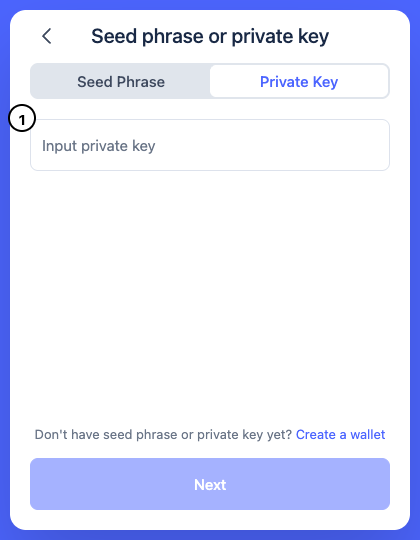
\includegraphics[width=\linewidth,height=.42\textheight,keepaspectratio]{assets/wallet-import-3-crop.png}\par 编号1表示钱包扩展中的私钥输入位置。输入框保持为空。\end{center}
本次更新保留原公网业主、中介和两位受托人的地址。角色地址与网络账户不是由网页按钮临时生成的。普通钱包可以作为投资者申请资格。完整演练中的投资者A/B和受托人A/B各使用独立账户。

两位受托人的普通登录角色相同，但钱包地址不同。服务事件达到固定快照30\%支持门槛后，需要两名不同受托人分别批准收款方变更。同一地址重复操作不能替代第二名受托人。

\clearpage\begin{landscape}
\subsection{角色账户 1}
\textbf{业主}\par
\nolinkurl{0xadC4920e9036dadC146ba1aF84fb1475C612E15b}\par
私钥由演示负责人通过内部渠道提供，不包含在本源码文档中。

\textbf{中介机构}\par
\nolinkurl{0xcee71e610f50435B8C9B0B25d3D322a5E184423a}\par
私钥由演示负责人通过内部渠道提供，不包含在本源码文档中。

\end{landscape}
\clearpage\begin{landscape}
\subsection{角色账户 2}
\textbf{投资者 A}\par
\nolinkurl{0x34cAACf0E56129F461afA460cDa3B220a3bfe2F2}\par
私钥由演示负责人通过内部渠道提供，不包含在本源码文档中。

\textbf{投资者 B}\par
\nolinkurl{0xcC245B1140F25b91BD8C13B05d9516A85da75605}\par
私钥由演示负责人通过内部渠道提供，不包含在本源码文档中。

\end{landscape}
\clearpage\begin{landscape}
\subsection{角色账户 3}
\textbf{受托管理人 A}\par
\nolinkurl{0x2641feCc09b01C7C482F51deDB28372daa41326a}\par
私钥由演示负责人通过内部渠道提供，不包含在本源码文档中。

\textbf{受托管理人 B}\par
\nolinkurl{0xfcf63f6E1100C4dD1bd0630C358848d990E33e64}\par
私钥由演示负责人通过内部渠道提供，不包含在本源码文档中。

\end{landscape}
\clearpage\section{网站、网络与区块链浏览器}
\subsection{公开首页}
\url{https://mengzhon001.github.io/deye-rwa-demo}\par
\subsection{业务应用}
\url{https://ski-june-reached-oldest.trycloudflare.com/app/}\par
\subsection{区块链浏览器}
\url{https://polyphonic-reduction-gratuit-pic.trycloudflare.com}\par
\subsection{钱包 RPC}
\url{https://sarah-reggae-calling-pat.trycloudflare.com}\par
测试网络Chain ID为20261008，Gas代币为DETH。首次登录时允许添加此网络，并核对当前RPC地址。隧道地址变化时需要更新RPC，但链编号、钱包地址和原链余额不变。127.0.0.1只指向使用者自己的电脑，远程同事不应使用本机端口地址。

在业务交易确认后点击交易哈希，即可打开对应的Blockscout页面。也可以将完整交易哈希、钱包地址或合约地址粘贴到浏览器顶部的搜索框。先核对状态、发送者、目标合约和区块，再检查代币转账与事件。登录和协议消息签名属于链下步骤，不会产生交易记录。

\clearpage\section{Base Sepolia 独立公链测试}
原公网演示继续用于完整生命周期演练。Base Sepolia 是另一个独立环境，用于检验公共链的合约和钱包交易。两者沿用同一组角色地址，但合约、余额和业务记录相互独立。后文的完整生命周期操作图以私链演示为例，公链测试应遵循本节的实际时间和资金限制。

\subsection{独立入口与网络配置}
公链测试应用\par\url{https://icq-attorneys-frontpage-weekends.trycloudflare.com/app/}\par
公链浏览器\par\url{https://base-sepolia.blockscout.com}\par
钱包 RPC\par\url{https://sepolia.base.org}\par
Chain ID 为 84532，Gas 代币为测试 ETH，支付代币为 Circle 测试 USDC。首页的 Launch App 仍然打开原演示。请点击独立的 Base Sepolia 入口，并在钱包中核对网络后登录。

\nolinkurl{0x036CbD53842c5426634e7929541eC2318f3dCF7e}\par
上述地址是本环境使用的官方 Circle 测试 USDC，精度为六位。它与私链 mUSDC 不同。测试币没有货币价值，不能将其他链上的余额直接用于本链认购。

\subsection{环境构成与数据流}
\begin{center}\begin{tikzpicture}[>=Latex,node distance=1cm,box/.style={draw,align=center,text width=4.5cm,minimum height=1.3cm}]
\node[box] (web) at (0,0) {GitHub 首页与文档};
\node[box] (app) at (6,0) {独立 Mac 业务应用};
\node[box] (wallet) at (6,-2.5) {Rabby 钱包};
\node[box] (chain) at (0,-5) {Base Sepolia 公共链};
\node[box] (explorer) at (6,-5) {公共 Blockscout};
\draw[->] (web)--(app);
\draw[->] (app)--(wallet);
\draw[->] (wallet)--(chain);
\draw[->] (app)--(chain);
\draw[->] (chain)--(explorer);
\end{tikzpicture}\end{center}
业务页面通过 HTTPS 连接独立后端。钱包签署交易后将其广播到 Base Sepolia，后端核对回执和事件，公共浏览器随后索引记录。本环境没有部署 Anvil，也不依赖原私链的 RPC 隧道。

\subsection{资金准备与认购操作}
请先使用页面的测试资金入口打开官方水龙头，选择 Base Sepolia，并向当前角色地址领取测试 ETH 和 Circle 测试 USDC。领取可能需要服务方登录或受到频率限制。系统本身不能增发 Circle USDC。确认到账后，返回页面并刷新余额。私钥只应输入钱包扩展，不应输入水龙头或业务网站。

\url{https://portal.cdp.coinbase.com/products/faucet}\par\url{https://faucet.circle.com/}\par
投资者选择募集中产品并申请资格。中介批准资格后，投资者填写金额，先批准对应 USDC 额度，再确认认购交易。募集开放时可以追加认购，每次追加后中介必须重新审核累计金额。结算前取消认购会退回本人全部累计托管款。认购进入托管并不等于已经取得 DRS。

结算继续要求有效估值、订单审批、募集门槛以及足够的购买款和初始留存。合约会自动留存10\%，不需要用户另行转账。少量测试币可以用于检查授权、认购、审核和退款，不能据此声称已经完成需要更多资金的发行结算。

\subsection{真实时间与测试范围}
公共链不能由应用提前推进时间。月度缴费需要产品已经结算，并到达对应服务期末。六个月转让锁定、赎回通知期和到期时间也保持不变。页面因此不提供重置和时间推进。完整生命周期演示仍应使用原公网私链环境。

业主月度缴费使用 Circle 测试 USDC。售电回款仍作为单独披露的经济模拟，其代币必须由独立资金账户预先持有。电站数据使用固定采集时间的真实记录回放，电价和未来现金流继续属于模型假设。本次部署未加入 Oracle，不能把报告上链解释为 API 数据已获得独立验证。

\clearpage
\subsection{交易核对与恢复}
交易提交后，请使用其哈希在公共浏览器核对发送者、目标合约、调用方法、事件和 USDC 转移。后端和钱包使用的 RPC 可能在不同时刻查到同一笔交易。遇到等待提示时应保留原哈希，重试原操作的确认，不要再次付款。浏览器索引稍有延迟并不表示交易失败。

电站凭证合约\par\nolinkurl{0xf17FFEAb245CebCd260a2E6aFAe90A43F2749176}\par
收益权资产池\par\nolinkurl{0xB84F6E2EB3b9e63bBE447190dF268c49D617A445}\par
月度缴费合约\par\nolinkurl{0xa2748E730069A38913b5E2e09a45C5aB546a0908}\par
\clearpage\begin{landscape}
\begin{center}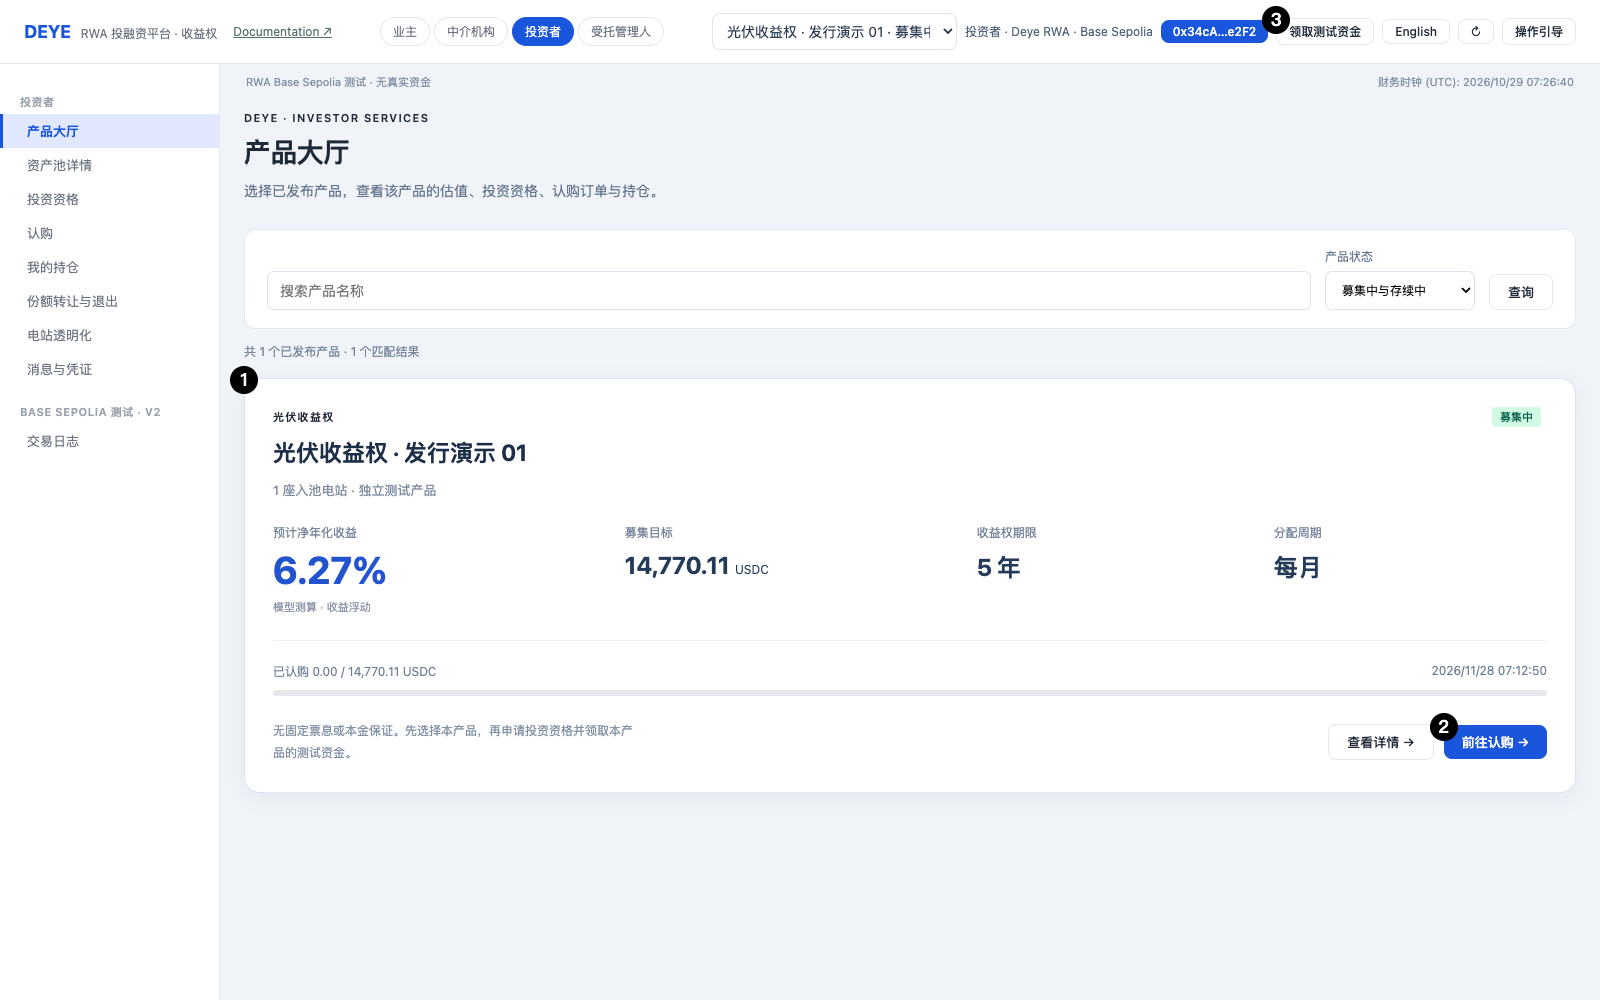
\includegraphics[width=\linewidth,height=.90\textheight,keepaspectratio]{assets/base-product.zh.png}\par 独立公链产品与网络信息。编号指向本次测试的产品、认购入口和测试资金入口。\end{center}
\end{landscape}
\clearpage\begin{landscape}
\begin{center}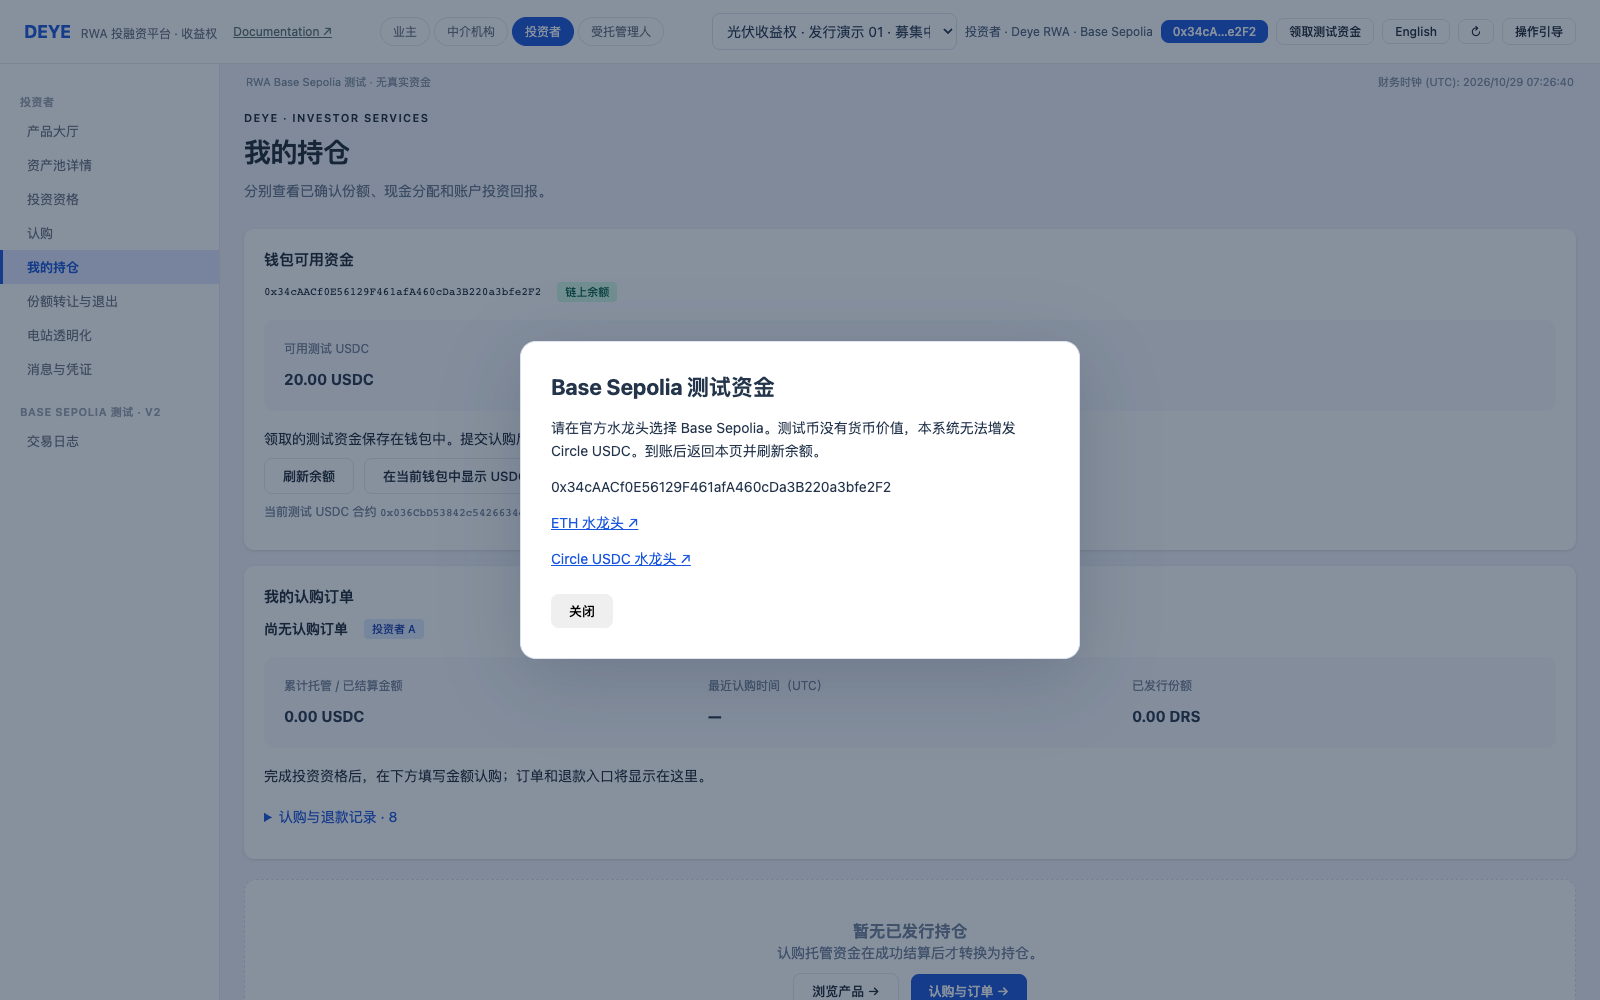
\includegraphics[width=\linewidth,height=.90\textheight,keepaspectratio]{assets/base-wallet.zh.png}\par 钱包余额与官方水龙头说明。此页面不会通过后台增发 Circle USDC。\end{center}
\end{landscape}
\clearpage\section{动态引导与交接}
首次进入角色时，业务介绍说明设备、收益权、资金和参与者之间的关系。右侧操作引导显示当前产品、对象、必要条件、处理人和预期结果。可以暂停或收起引导，再从顶部“操作引导”恢复。完成状态来自业务与链上记录，不由“下一步”按钮决定。

参与者模式关注本人任务及交接等待。四角色演示模式可查看其他角色的待办，并打开角色登录入口，但仍需要切换到对应钱包并重新签名。它不是代签模式，也不会让投资者钱包获得中介权限。

每次点击“定位操作”都会进入相关页面并指向按钮、字段或阻塞条件。条件不足时，弹窗应提供具体处理入口。需要他人审批时切换到所示角色，需要补齐估值时进入报告编制，需要未来日期时由中介确认受控时间推进。只读查看不会被描述为不能执行的付款。

月度流程中，受托尚未批准本期估值时，应先完成审批。中介宣告新分配且存在实际可领取金额后，引导才交接到投资者。已经领取完的旧分配不会继续占据当前任务。投资者可以核对历史已领取金额与本期未宣告状态，并分别查看剩余净值。

\clearpage
\subsection{业务介绍与任务入口}
\begin{center}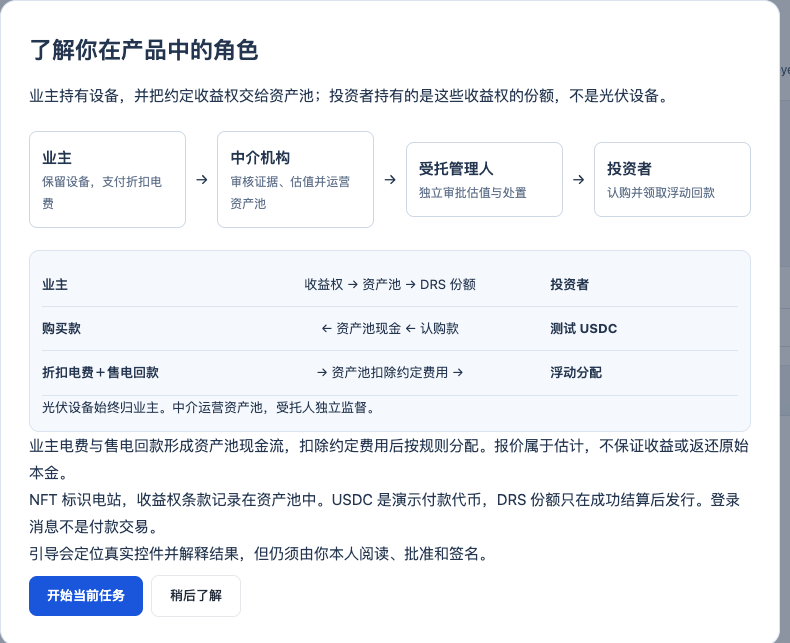
\includegraphics[width=\linewidth,height=.62\textheight,keepaspectratio]{assets/guide-overview.zh.png}\par 阅读后可开始当前任务，也可选择稍后了解。引导不会替参与者签名。\end{center}
\clearpage\begin{landscape}
\section{应用入口}
\subsection{A0 业务应用访问}
本步由所有测试同事操作。进入GitHub首页后，点击编号1所示Launch App。首页和文档无需钱包登录。

操作成功后，浏览器进入当前业务HTTPS入口并显示角色弹窗。下一步，使用对应测试钱包登录。

若入口提示离线，应联系演示负责人启动Mac服务与隧道，不要把Blockscout地址当作业务入口。

\begin{center}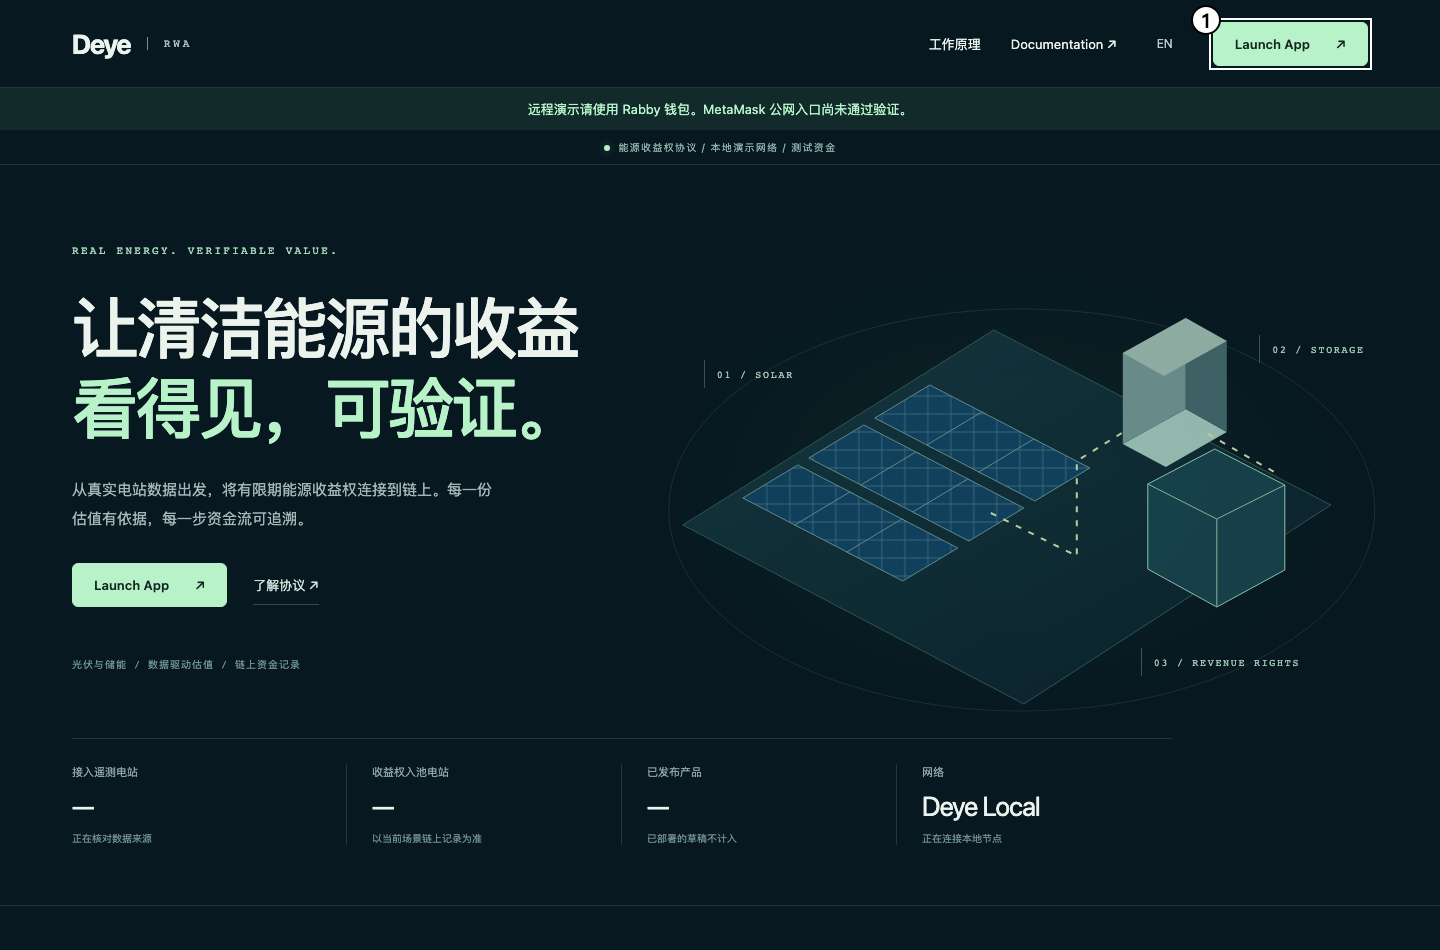
\includegraphics[width=\linewidth,height=.60\textheight,keepaspectratio]{assets/54-home.png}\par 编号标出操作位置。插图来自隔离演练，金额和状态以当前产品为准。\end{center}
\end{landscape}
\clearpage\begin{landscape}
\subsection{A1 选择角色并登录}
本步由本次操作对应的参与者操作。进入首页的Launch App入口后，在弹窗中点击所需角色，再在编号2处选择Rabby，最后点击编号3处连接钱包并登录。钱包请求出现后，核对地址、域名和链编号，再确认签名。

操作成功后，页面进入所选角色工作台。登录消息签名不扣除USDC，也不会产生业务交易。下一步，该角色按左侧导航开始业务。

编号1是角色选项。若提示地址不具备权限，应换到本章列出的对应账户，不要重复点击连接按钮。

\begin{center}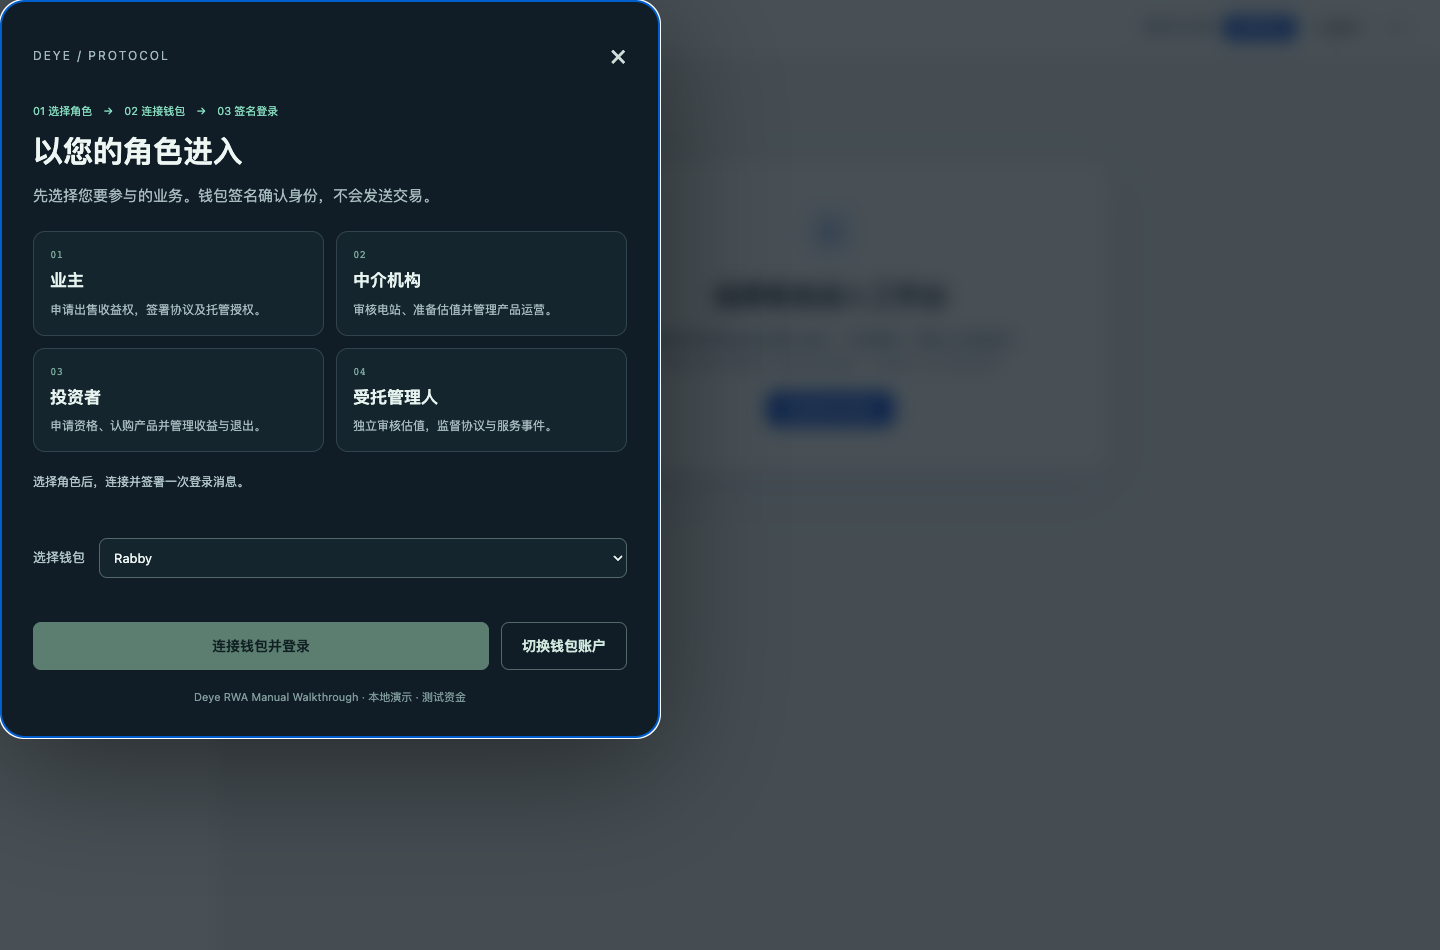
\includegraphics[width=\linewidth,height=.60\textheight,keepaspectratio]{assets/01-role-login.png}\par 编号标出操作位置。插图来自隔离演练，金额和状态以当前产品为准。\end{center}
\end{landscape}
\clearpage\begin{landscape}
\subsection{A2 创建新的发行草稿}
本步由中介机构操作。进入页面顶部的“创建新一期”后，点击创建新一期，填写产品名并确认仅用于测试，再点击编号1部署并开始发行。

操作成功后，系统部署独立产品合约并切换到新草稿。旧产品的退款和交易仍属于旧合约。下一步，业主在顶部选择同一个新产品后申请。

已停止募集的体验产品不能继续发行。创建新一期用于重新走发行流程，不应为了演示而删除同事原来的托管订单。

\begin{center}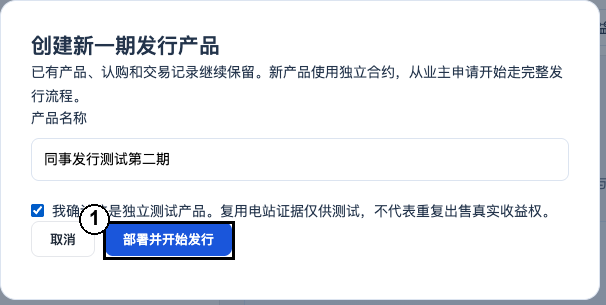
\includegraphics[width=\linewidth,height=.37\textheight,keepaspectratio]{assets/52-new-product-context.png}\par 编号标出操作位置。插图来自隔离演练，金额和状态以当前产品为准。\end{center}
\begin{center}
\includegraphics[width=.7\linewidth,height=1.55cm,keepaspectratio]{assets/52-new-product-detail.png}\end{center}
\end{landscape}
\clearpage\begin{landscape}
\subsection{A3 领取当前产品测试资金}
本步由本次登录的参与者操作。进入页面顶部后，点击编号1处领取测试资金，再到认购页核对余额。

操作成功后，当前地址取得演示燃料币和所选产品的测试USDC。下一步，投资者确认资格后认购，其他角色继续待办。

水龙头只是准备演示资金，不是认购，也不会增加DRS。切换到新产品后应重新检查它自己的USDC合约余额。

\begin{center}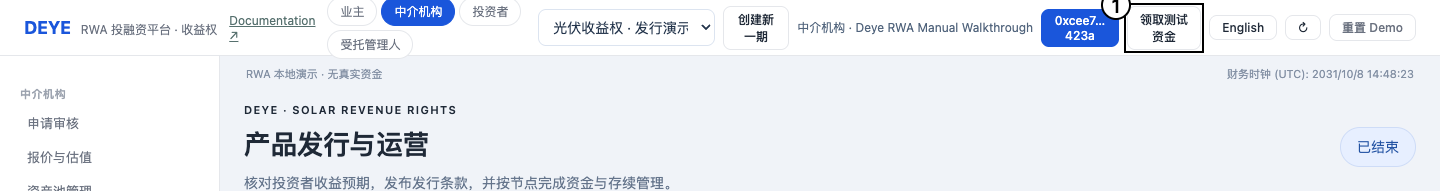
\includegraphics[width=\linewidth,height=.37\textheight,keepaspectratio]{assets/53-faucet-context.png}\par 编号标出操作位置。插图来自隔离演练，金额和状态以当前产品为准。\end{center}
\begin{center}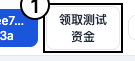
\includegraphics[width=.7\linewidth,height=1.55cm,keepaspectratio]{assets/53-faucet-detail.png}\end{center}
\end{landscape}
\clearpage\begin{landscape}
\section{申请、估值与协议}
\subsection{B1 核对电站与证据来源}
本步由业主操作。进入“我的电站”和“电站详情”后，先在列表确认电站名称，再点击编号1所示详情入口。

操作成功后，详情页显示站点、设备、历史电量和采集时间。下一步，业主提交收益权申请。

“我的电站”是列表，“电站详情”是单站看板。监控时间与合约财务时间分别记录。

\begin{center}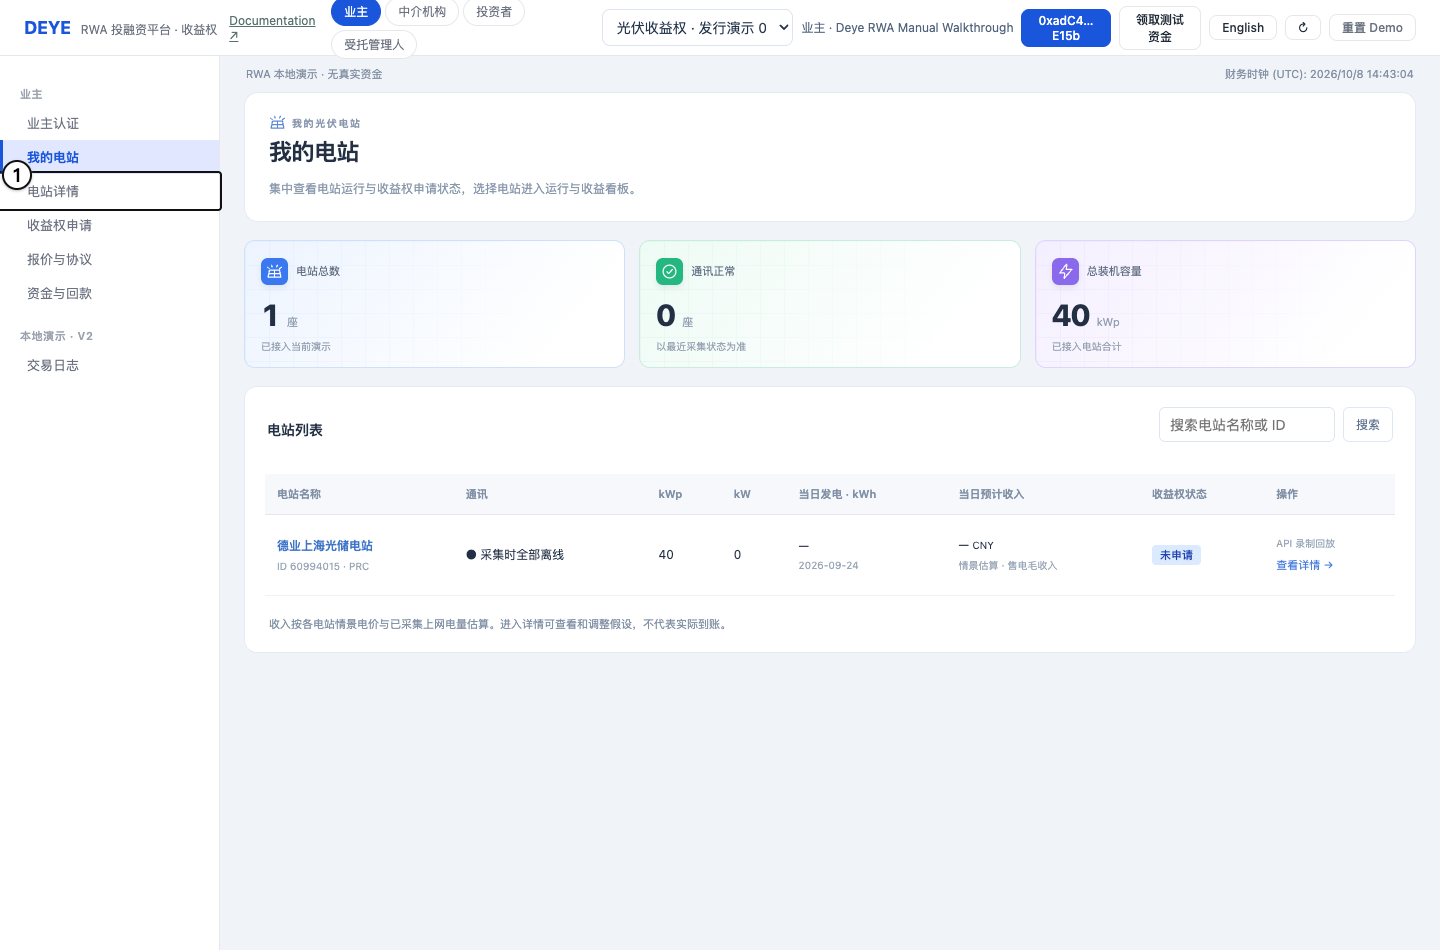
\includegraphics[width=\linewidth,height=.60\textheight,keepaspectratio]{assets/02-station-list.png}\par 编号标出操作位置。插图来自隔离演练，金额和状态以当前产品为准。\end{center}
\end{landscape}
\clearpage\begin{landscape}
\subsection{B2 阅读电站详情}
本步由业主操作。进入“电站详情”后，在编号1附近核对电站名称、容量、数据模式和更新时间，再阅读历史图表。

操作成功后，确认自己正在使用的电站证据。下一步，业主进入收益权申请。

ALL\_OFFLINE表示API返回的采集状态，不代表链上产品失效。回放中的离线状态属于当时记录，不应被解释成当前实时状态。

\begin{center}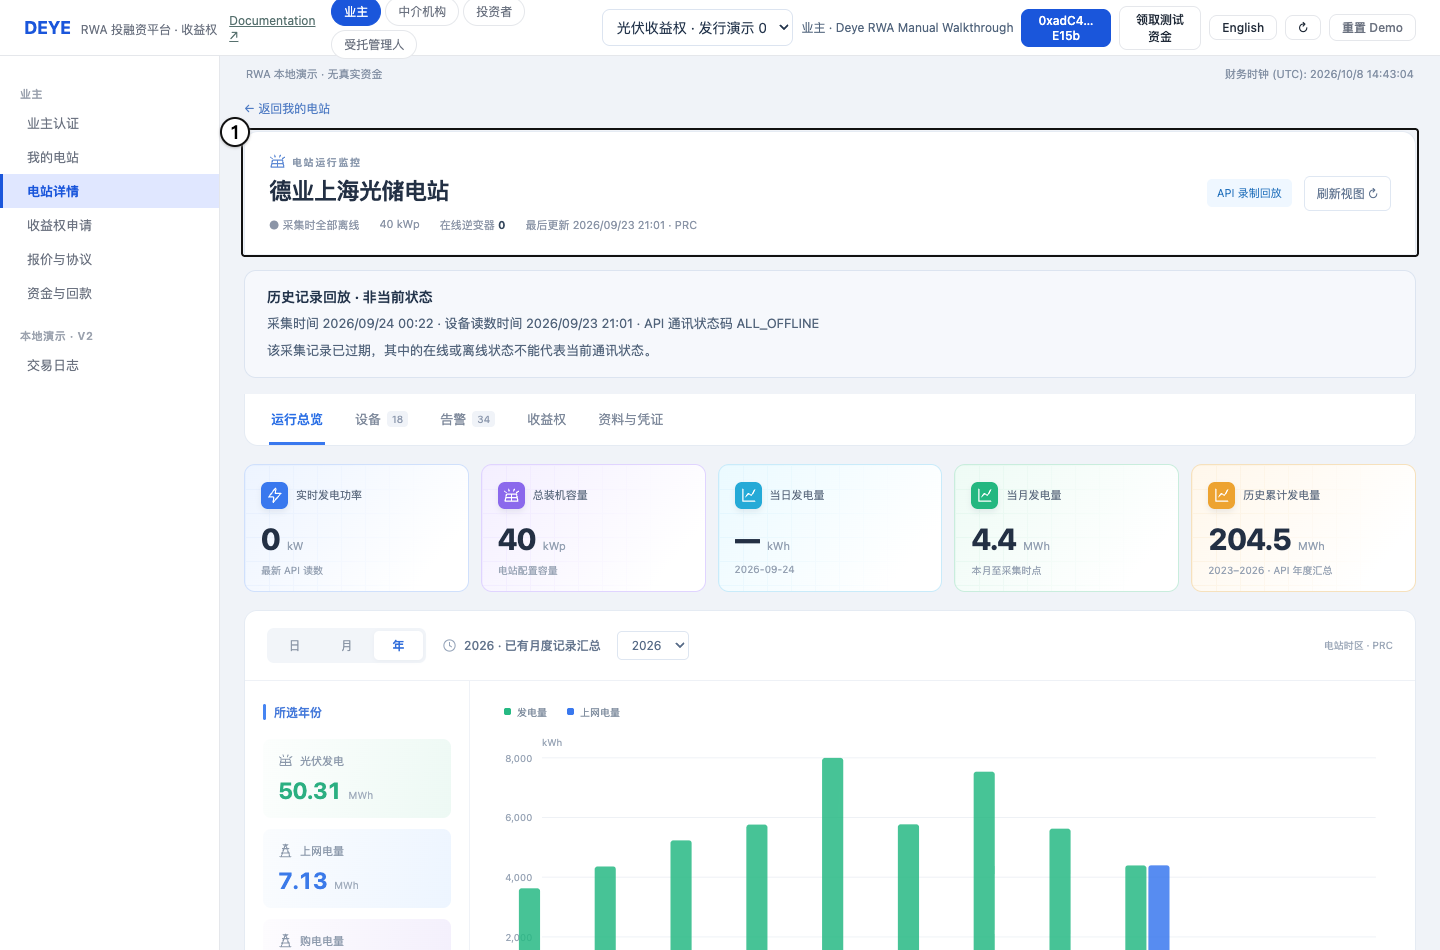
\includegraphics[width=\linewidth,height=.60\textheight,keepaspectratio]{assets/03-station-detail.png}\par 编号标出操作位置。插图来自隔离演练，金额和状态以当前产品为准。\end{center}
\end{landscape}
\clearpage\begin{landscape}
\subsection{B3 提交收益权申请}
本步由业主操作。进入“收益权申请”后，选择电站，填写收入归集安排和补充说明，然后点击编号1处的提交按钮。

操作成功后，系统生成一条申请及其编号，申请详情显示等待中介审核。下一步，中介机构在申请队列处理。

本步只保存资料与证据摘要，不铸造电站NFT，不发行DRS。

\begin{center}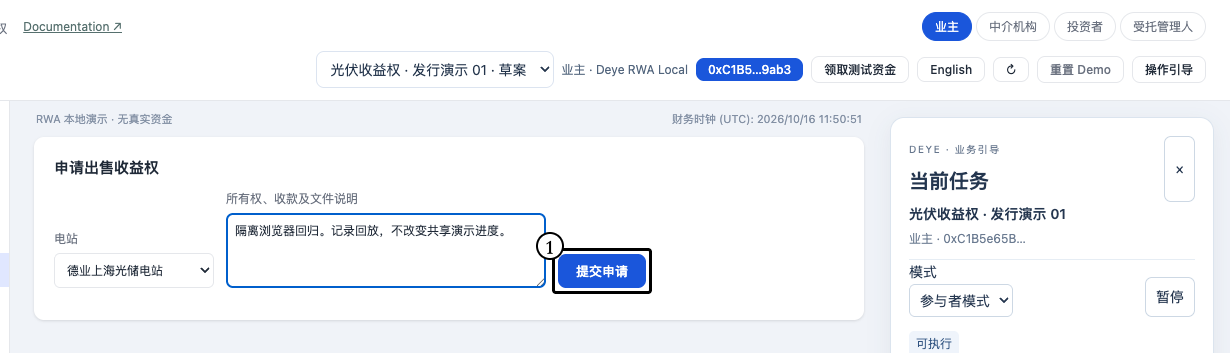
\includegraphics[width=\linewidth,height=.37\textheight,keepaspectratio]{assets/01-owner-apply.zh-context.png}\par 编号1标出本步需要核对或提交的控件。\end{center}
\begin{center}
\includegraphics[width=.7\linewidth,height=1.55cm,keepaspectratio]{assets/01-owner-apply.zh-detail.png}\end{center}
\end{landscape}
\clearpage\begin{landscape}
\subsection{B4 待审核申请查询}
本步由中介机构操作。进入“申请审核”后，在列表中按申请编号和状态找到记录，点击编号1处进入详情。

操作成功后，详情展示申请资料、证据、审核动作和下一步。下一步，中介机构审核资料。

\begin{center}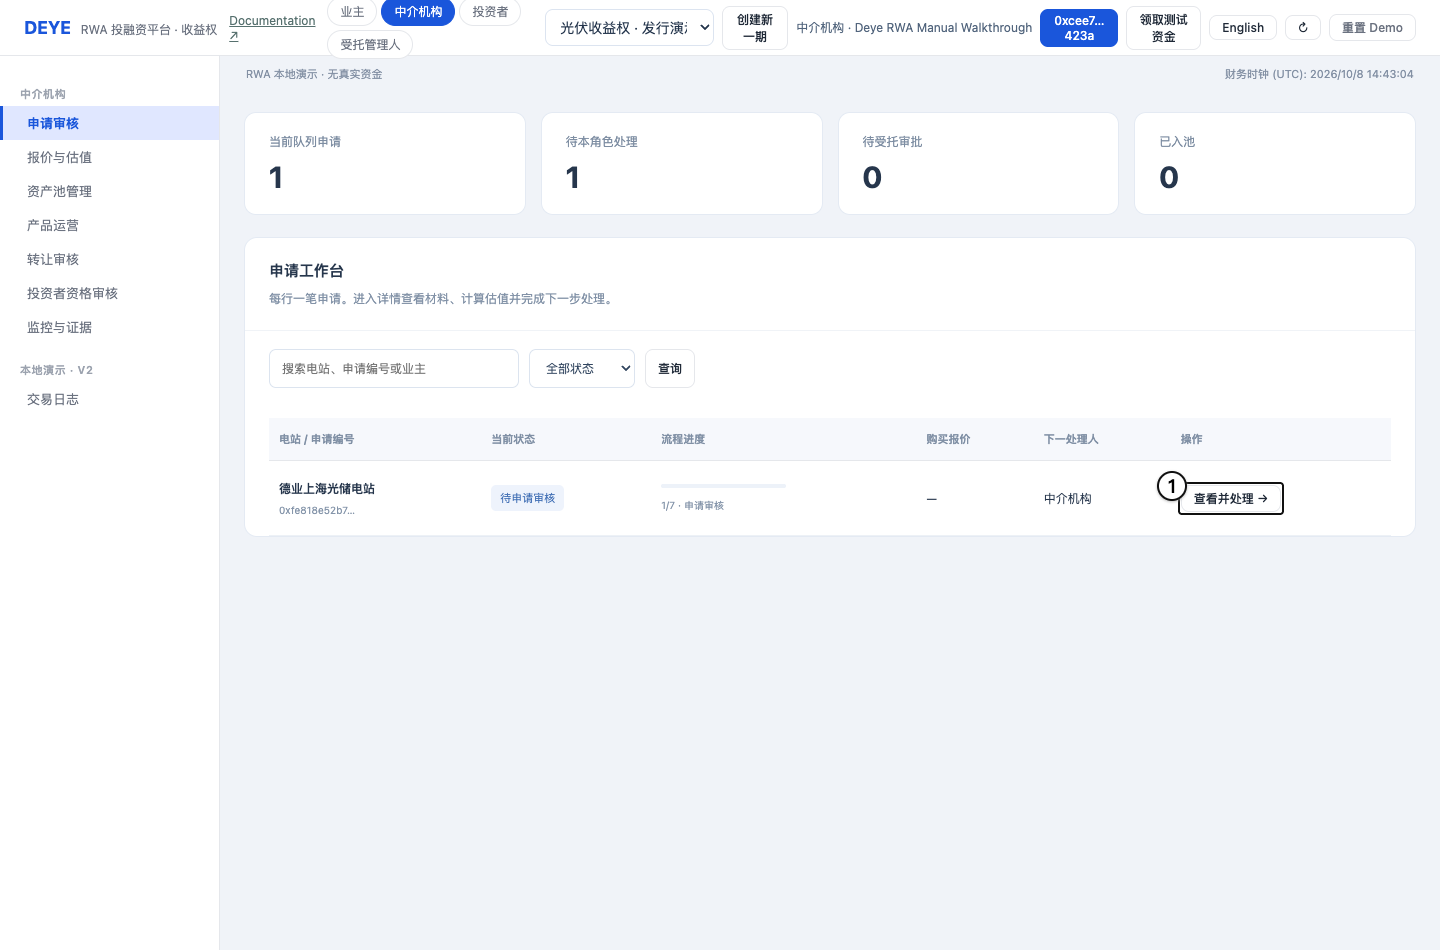
\includegraphics[width=\linewidth,height=.60\textheight,keepaspectratio]{assets/05-review-list.png}\par 编号标出操作位置。插图来自隔离演练，金额和状态以当前产品为准。\end{center}
\end{landscape}
\clearpage\begin{landscape}
\subsection{B5 申请资料审核}
本步由中介机构操作。进入申请详情的审核区后，核对电站身份及收款责任，选择审核通过并填写意见，再点击编号1。资料不完整时应要求补充。

操作成功后，通过的申请进入报价流程；补充资料的申请回到业主，拒绝的申请不继续发行。下一步，中介机构生成估值报价。

资料审核通过不等于报价获批，也不产生投资者份额。

\begin{center}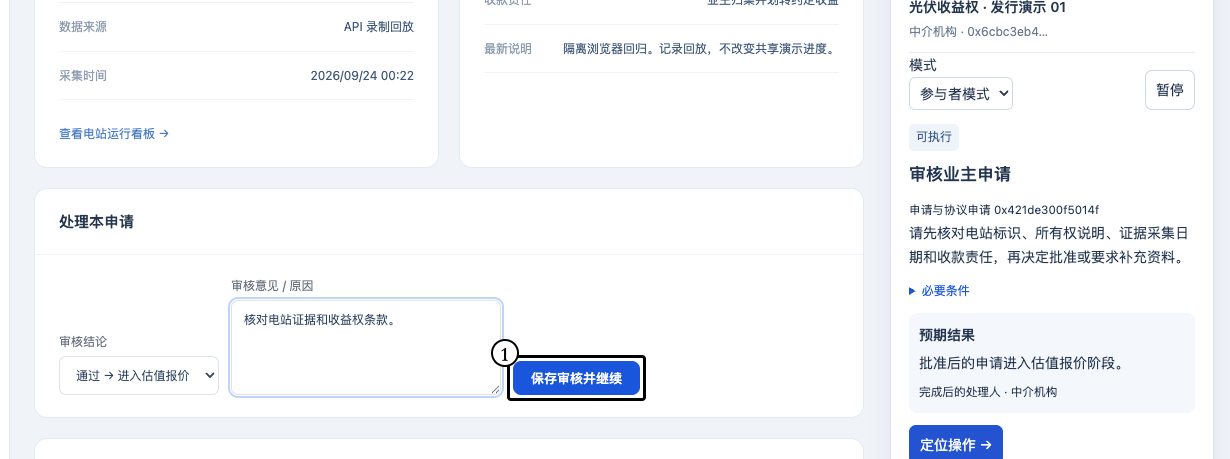
\includegraphics[width=\linewidth,height=.37\textheight,keepaspectratio]{assets/02-agent-review.zh-context.png}\par 编号1标出本步需要核对或提交的控件。\end{center}
\begin{center}
\includegraphics[width=.7\linewidth,height=1.55cm,keepaspectratio]{assets/02-agent-review.zh-detail.png}\end{center}
\end{landscape}
\clearpage\begin{landscape}
\subsection{B6 生成收益权报价}
本步由中介机构操作。进入“报价与估值”的申请详情后，选择历史季节性基线，核对电价、业主支付比例、交付系数、费用和汇率，记录基线选择依据并确认数据口径，最后点击编号1。

操作成功后，系统保存60期现金流、折现估值、报价及模型和证据摘要。下一步，受托管理人审核报价。

近期上网量超过发电量时不能选择近期比例估算。先试算并审阅，再提交正式报价，不要把折现率宣传成投资收益率。

\begin{center}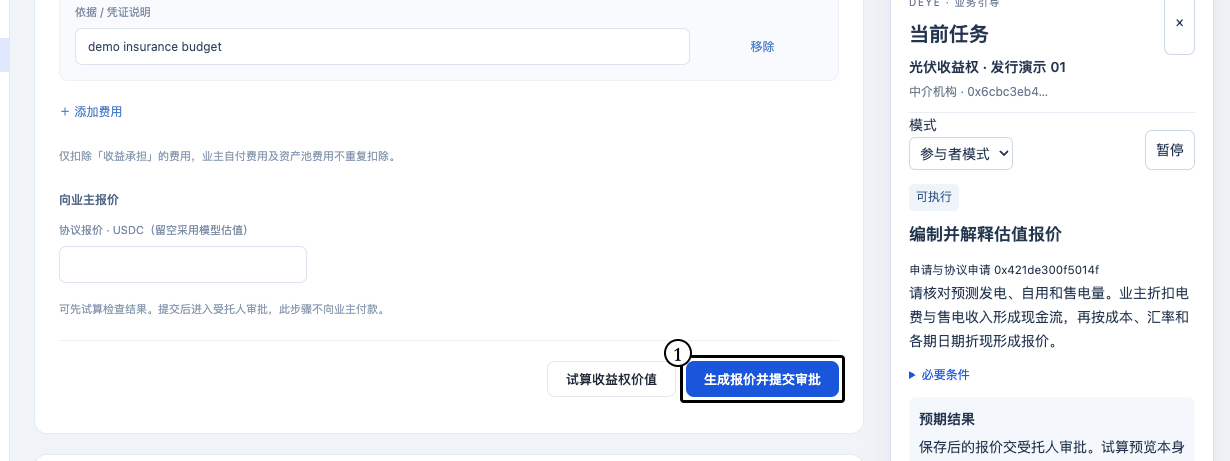
\includegraphics[width=\linewidth,height=.37\textheight,keepaspectratio]{assets/03-agent-offer.zh-context.png}\par 编号1标出本步需要核对或提交的控件。\end{center}
\begin{center}
\includegraphics[width=.7\linewidth,height=1.55cm,keepaspectratio]{assets/03-agent-offer.zh-detail.png}\end{center}
\end{landscape}
\clearpage\begin{landscape}
\subsection{B7 独立批准报价}
本步由受托管理人A操作。进入“审核队列”的报价详情后，核对收入分配、估值有效期和暂定标记，阅读基线依据，在确认接受暂定估算后点击编号1。

操作成功后，当前报价得到独立审批，可以交由业主接受。下一步，业主查看报价并确认。

批准的是这份有明确摘要的报告。数据、模型或购买价格变化后，不能沿用旧审批。

\begin{center}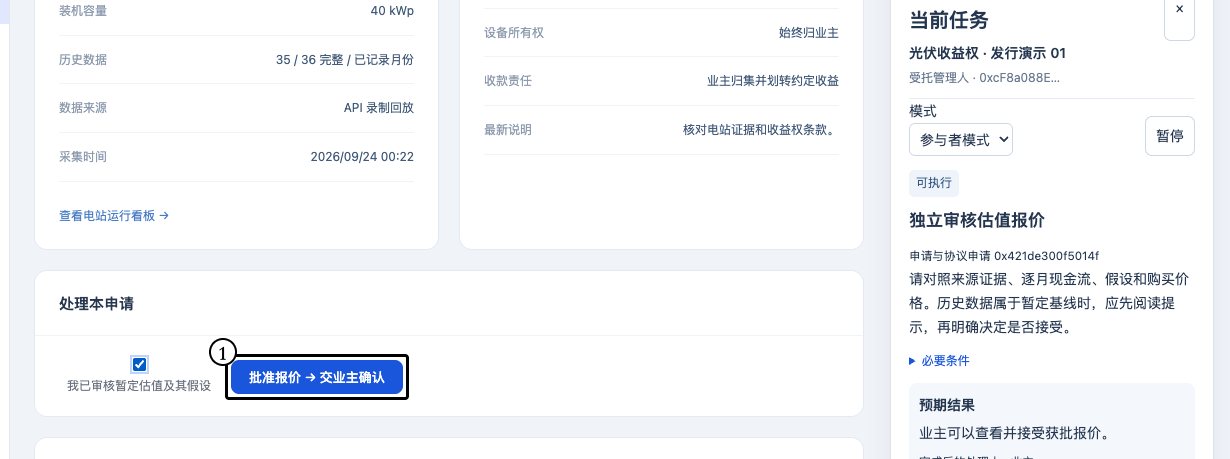
\includegraphics[width=\linewidth,height=.37\textheight,keepaspectratio]{assets/04-trustee-approve-offer.zh-context.png}\par 编号1标出本步需要核对或提交的控件。\end{center}
\begin{center}
\includegraphics[width=.7\linewidth,height=1.55cm,keepaspectratio]{assets/04-trustee-approve-offer.zh-detail.png}\end{center}
\end{landscape}
\clearpage\begin{landscape}
\subsection{B8 核对逐期现金流与电费优惠}
本步由业主操作。进入“报价与协议”后，沿时间轴从左向右查看各期发电量、上网量、交付自用量、业主付款、售电收入及现金流现值。

操作成功后，理解一次性收款与随后每月付费义务，确认报价依据。下一步，业主接受报价。

业主按电网价格80\%支付的是自用光伏部分；向电网实际购买的电量仍另行付费。

\begin{center}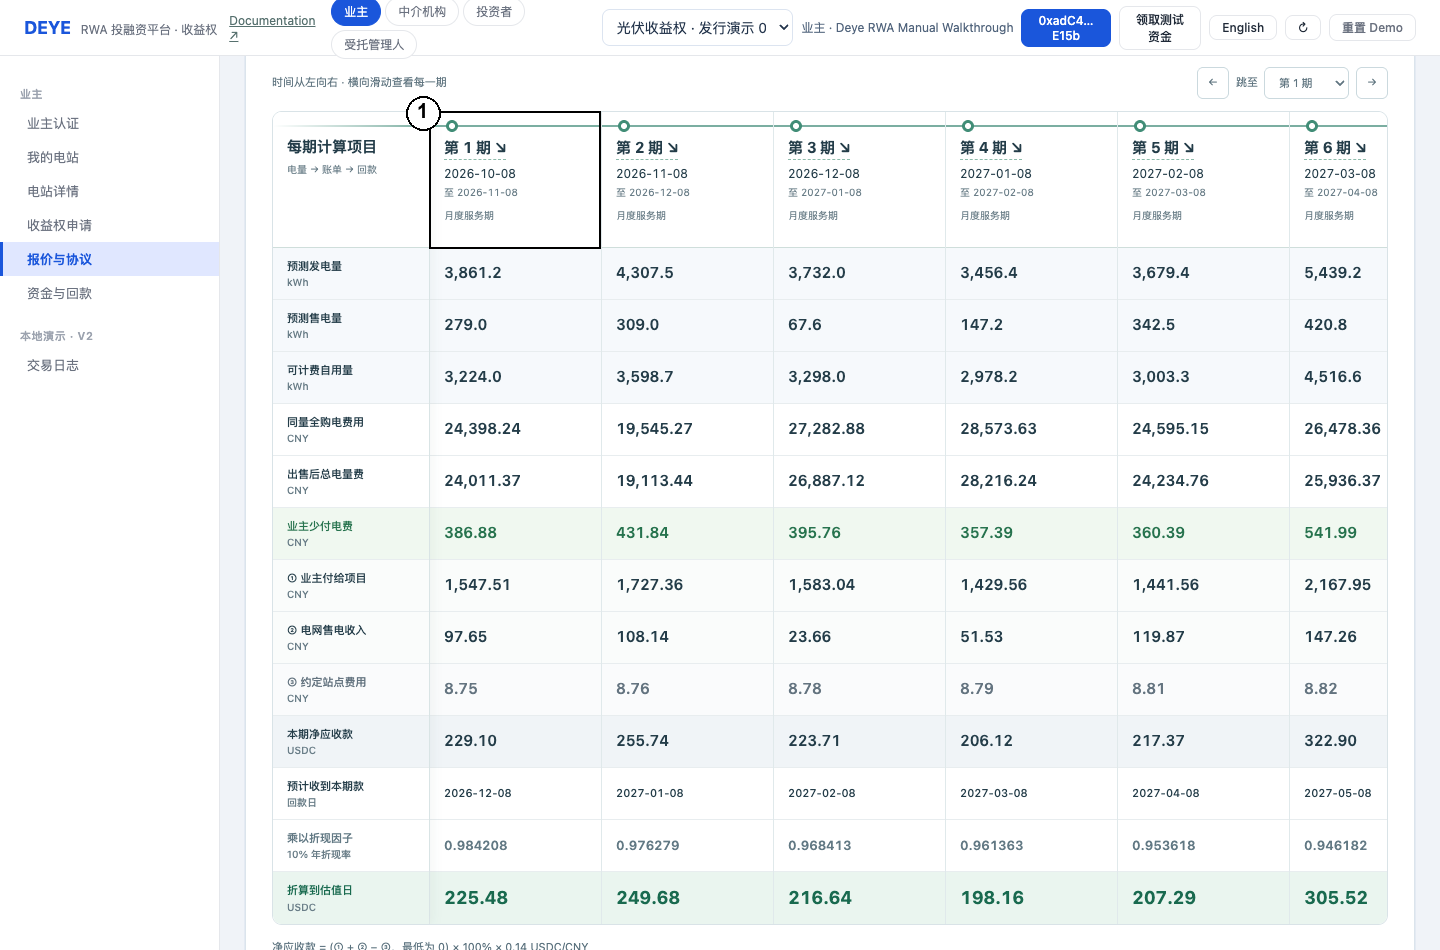
\includegraphics[width=\linewidth,height=.60\textheight,keepaspectratio]{assets/09-owner-timeline.png}\par 编号标出操作位置。插图来自隔离演练，金额和状态以当前产品为准。\end{center}
\end{landscape}
\clearpage\begin{landscape}
\subsection{B9 接受已批准的报价}
本步由业主操作。进入申请的报价详情后，确认购买价格和期限后点击编号1处接受报价。

操作成功后，经济条款冻结，详情允许签署协议。下一步，业主签署协议消息。

\begin{center}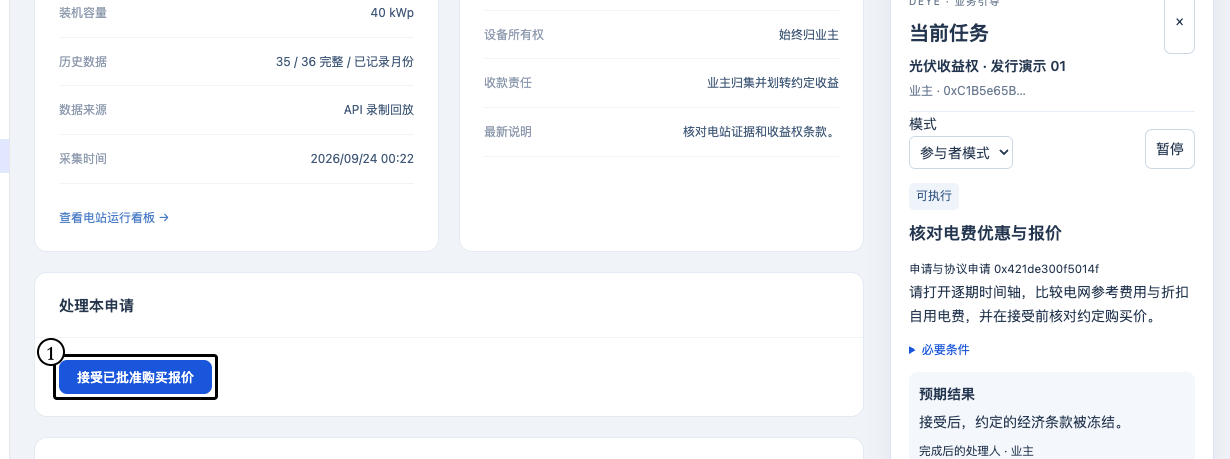
\includegraphics[width=\linewidth,height=.37\textheight,keepaspectratio]{assets/05-owner-accept.zh-context.png}\par 编号1标出本步需要核对或提交的控件。\end{center}
\begin{center}
\includegraphics[width=.7\linewidth,height=1.55cm,keepaspectratio]{assets/05-owner-accept.zh-detail.png}\end{center}
\end{landscape}
\clearpage\begin{landscape}
\subsection{B10 签署收益权协议}
本步由业主操作。进入同一申请的协议区后，点击编号1，在Rabby中阅读并签署绑定产品、站点、价格、比例、期限与链的协议消息。

操作成功后，后端记录签名和协议摘要，申请进入等待铸造状态。下一步，中介机构铸造电站凭证。

本步是消息签名，不收取认购款，也不等同于NFT已经铸造。

\begin{center}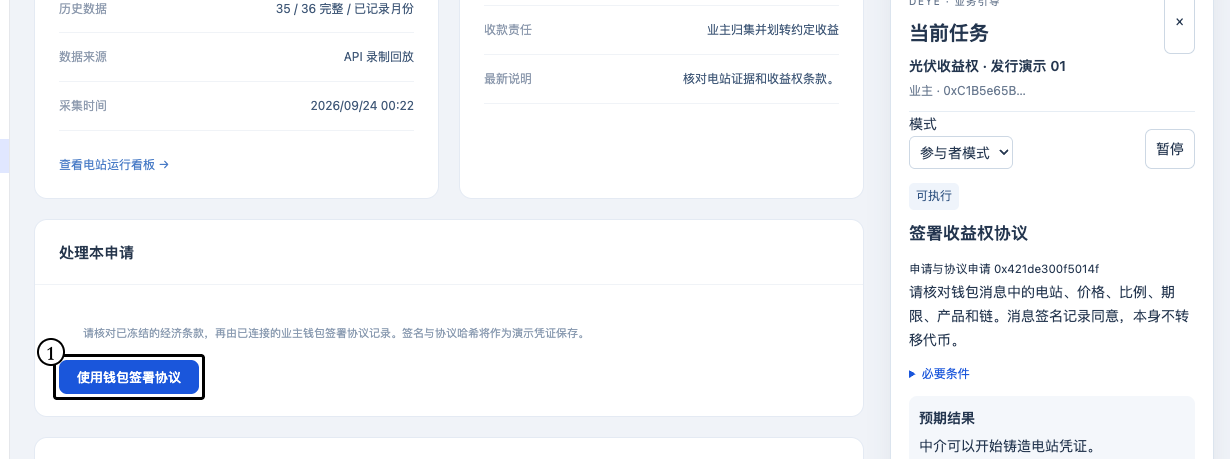
\includegraphics[width=\linewidth,height=.37\textheight,keepaspectratio]{assets/06-owner-sign.zh-context.png}\par 编号1标出本步需要核对或提交的控件。\end{center}
\begin{center}
\includegraphics[width=.7\linewidth,height=1.55cm,keepaspectratio]{assets/06-owner-sign.zh-detail.png}\end{center}
\end{landscape}
\clearpage\begin{landscape}
\section{凭证、入池与发行}
\subsection{C1 铸造电站身份凭证}
本步由中介机构操作。进入“资产池管理”的已签约申请后，点击编号1并在自己的钱包确认铸造交易。

操作成功后，站点NFT发给业主，系统记录Token ID和交易哈希。下一步，业主授权托管。

这是该申请首次产生的业务链上交易。凭证不转移设备法律所有权。

\begin{center}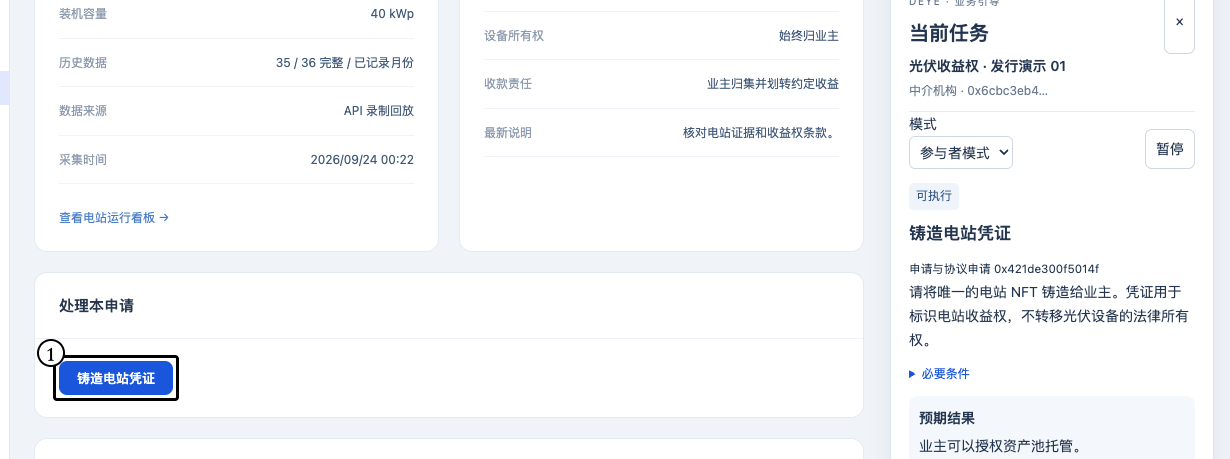
\includegraphics[width=\linewidth,height=.37\textheight,keepaspectratio]{assets/07-agent-mint-station.zh-context.png}\par 编号1标出本步需要核对或提交的控件。\end{center}
\begin{center}
\includegraphics[width=.7\linewidth,height=1.55cm,keepaspectratio]{assets/07-agent-mint-station.zh-detail.png}\end{center}
\end{landscape}
\clearpage\begin{landscape}
\subsection{C2 授权资产池托管}
本步由业主操作。进入“报价与协议”的托管待办后，核对资产池合约与Token ID，点击编号1并签署授权交易。

操作成功后，资产池取得接收这张站点NFT的权限。下一步，中介机构执行入池。

授权还不代表NFT已经进入资产池，中介仍需要执行下一步。

\begin{center}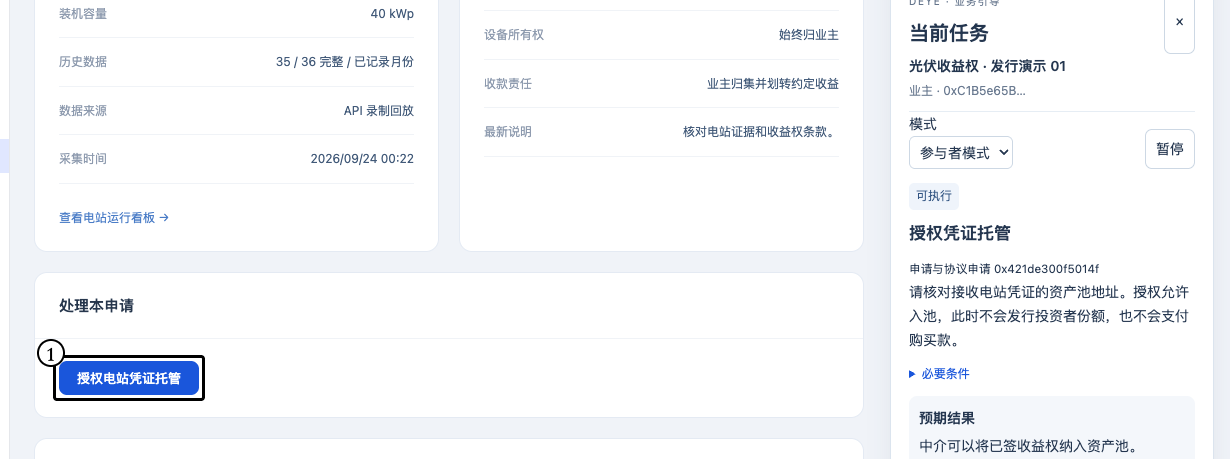
\includegraphics[width=\linewidth,height=.37\textheight,keepaspectratio]{assets/08-owner-custody-consent.zh-context.png}\par 编号1标出本步需要核对或提交的控件。\end{center}
\begin{center}
\includegraphics[width=.7\linewidth,height=1.55cm,keepaspectratio]{assets/08-owner-custody-consent.zh-detail.png}\end{center}
\end{landscape}
\clearpage\begin{landscape}
\subsection{C3 执行收益权入池}
本步由中介机构操作。进入“资产池管理”的已授权申请后，核对协议摘要和购买价，点击编号1完成入池。

操作成功后，NFT进入托管，收益权条款登记到资产池，投资者份额仍为零。下一步，中介机构提交资产池估值。

\begin{center}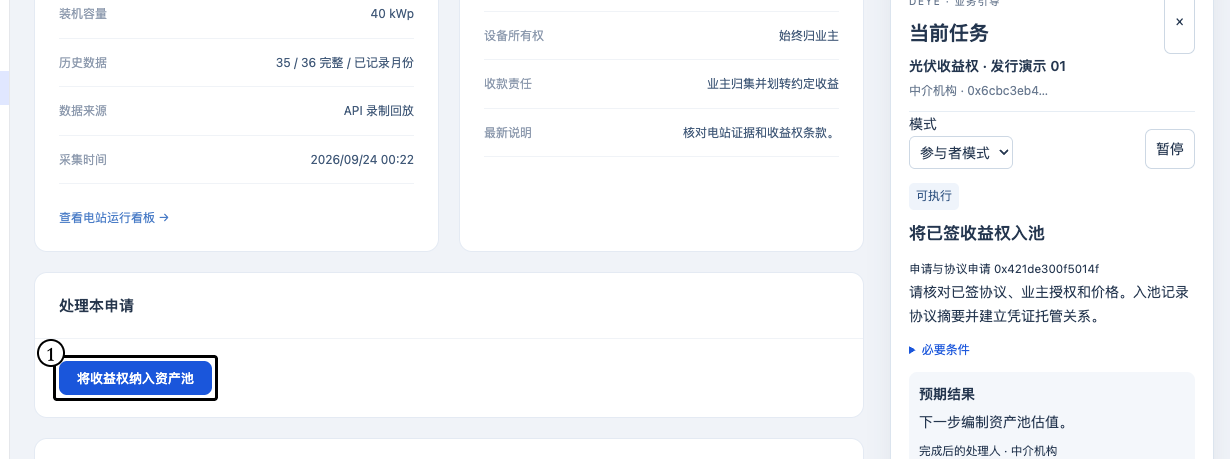
\includegraphics[width=\linewidth,height=.37\textheight,keepaspectratio]{assets/09-agent-admit.zh-context.png}\par 编号1标出本步需要核对或提交的控件。\end{center}
\begin{center}
\includegraphics[width=.7\linewidth,height=1.55cm,keepaspectratio]{assets/09-agent-admit.zh-detail.png}\end{center}
\end{landscape}
\clearpage\begin{landscape}
\subsection{C4 提交资产池估值}
本步由中介机构操作。进入“资产池管理”的估值区后，核对所选产品、全部入池收益权与池费用，然后点击编号1提交估值交易。

操作成功后，链上记录估值报告摘要、NAV及有效期。下一步，受托管理人A批准估值。

\begin{center}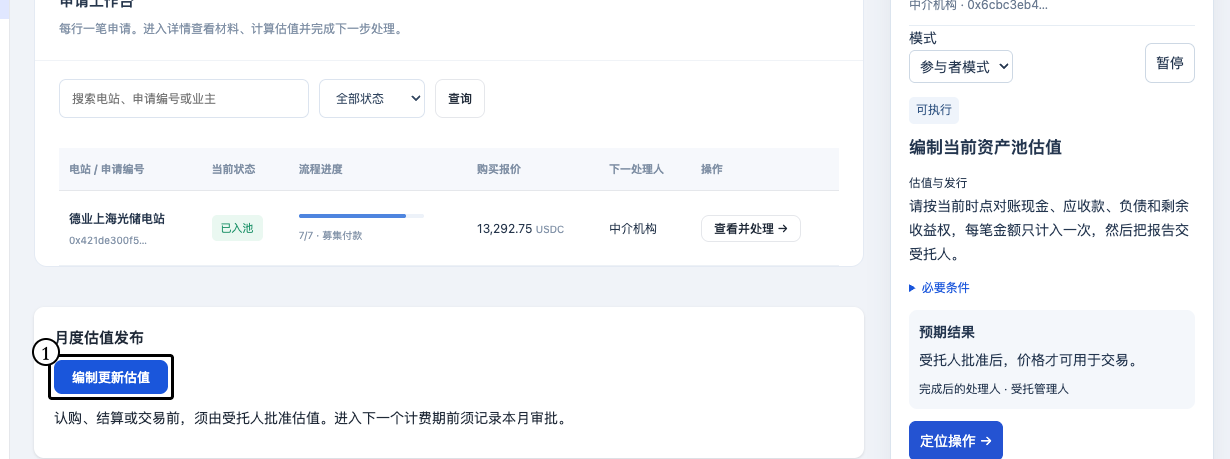
\includegraphics[width=\linewidth,height=.37\textheight,keepaspectratio]{assets/10-agent-prepare-valuation.zh-context.png}\par 编号1标出本步需要核对或提交的控件。\end{center}
\begin{center}
\includegraphics[width=.7\linewidth,height=1.55cm,keepaspectratio]{assets/10-agent-prepare-valuation.zh-detail.png}\end{center}
\end{landscape}
\clearpage\begin{landscape}
\subsection{C5 批准资产池估值}
本步由受托管理人A操作。进入“审核队列”的资产池估值区后，核对报告、现金、应收款、未来收益权和负债，确认暂定估算后点击编号1。

操作成功后，资产池取得当前有效的获批估值。下一步，中介机构发布募集。

\begin{center}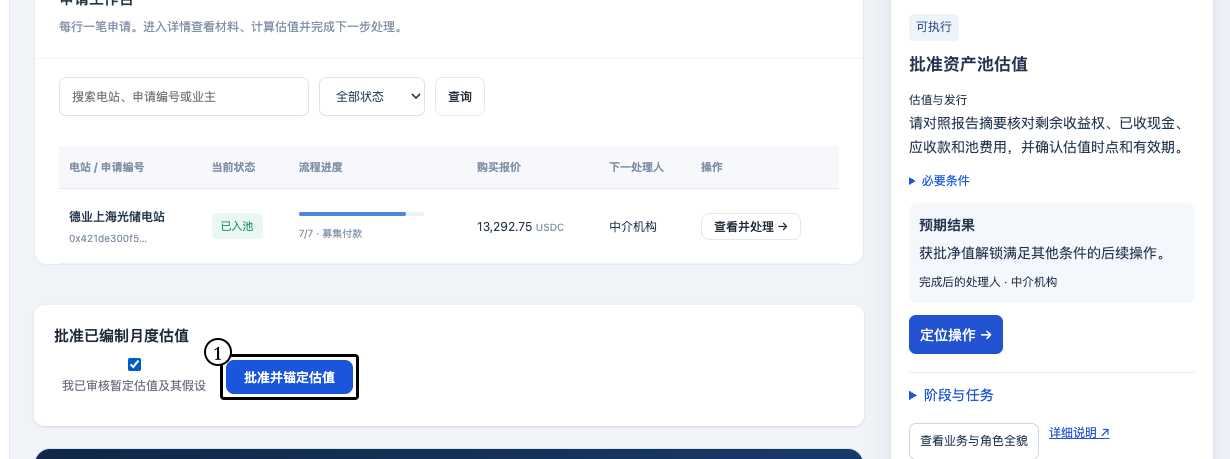
\includegraphics[width=\linewidth,height=.37\textheight,keepaspectratio]{assets/11-trustee-approve-valuation.zh-context.png}\par 编号1标出本步需要核对或提交的控件。\end{center}
\begin{center}
\includegraphics[width=.7\linewidth,height=1.55cm,keepaspectratio]{assets/11-trustee-approve-valuation.zh-detail.png}\end{center}
\end{landscape}
\clearpage\begin{landscape}
\subsection{C6 发布募集条款}
本步由中介机构操作。进入“产品运营”后，阅读预计净年化收益、现金分配时间轴、募集目标和购买资金要求，再点击编号1发布。

操作成功后，产品状态从草稿变为募集中，并进入产品大厅。下一步，投资者申请资格并认购。

发布募集不会发行DRS。不要点击“撤销募集”代替发布或结算，撤销会结束本次募集并转入退款。

\begin{center}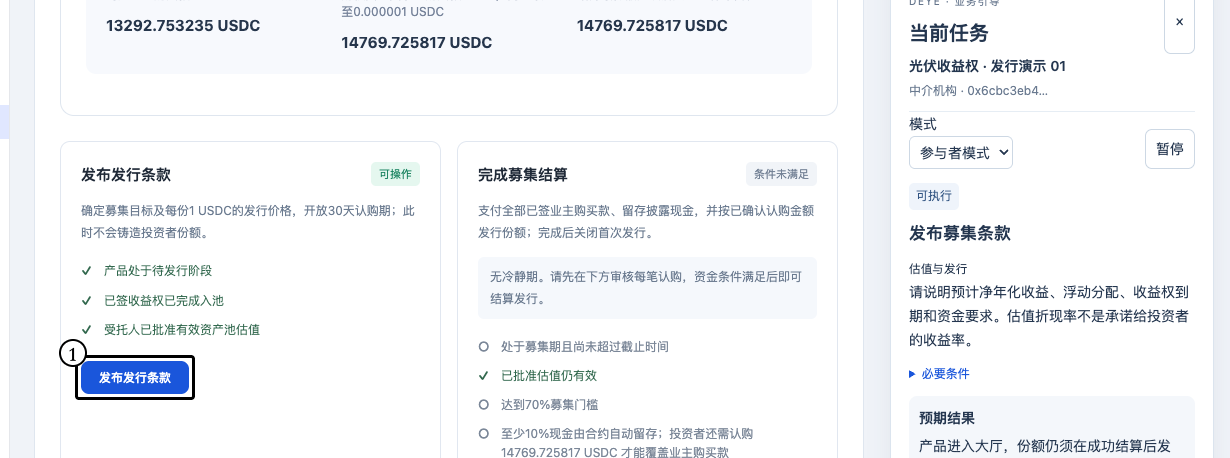
\includegraphics[width=\linewidth,height=.37\textheight,keepaspectratio]{assets/12-agent-publish.zh-context.png}\par 编号1标出本步需要核对或提交的控件。\end{center}
\begin{center}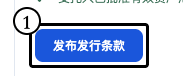
\includegraphics[width=.7\linewidth,height=1.55cm,keepaspectratio]{assets/12-agent-publish.zh-detail.png}\end{center}
\end{landscape}
\clearpage\begin{landscape}
\section{资格、认购与结算}
\subsection{D1 从产品大厅选择产品}
本步由投资者A或B操作。进入“产品大厅”后，核对状态、预计收益、期限及募集进度，点击编号1前往认购，或先进入详情阅读现金流。

操作成功后，应用切换到所选产品及其独立资格、余额和订单。下一步，投资者核对现金流与资格。

当前没有募集中产品时，应等待中介重新发布。已停止产品只能处理原订单退款。

\begin{center}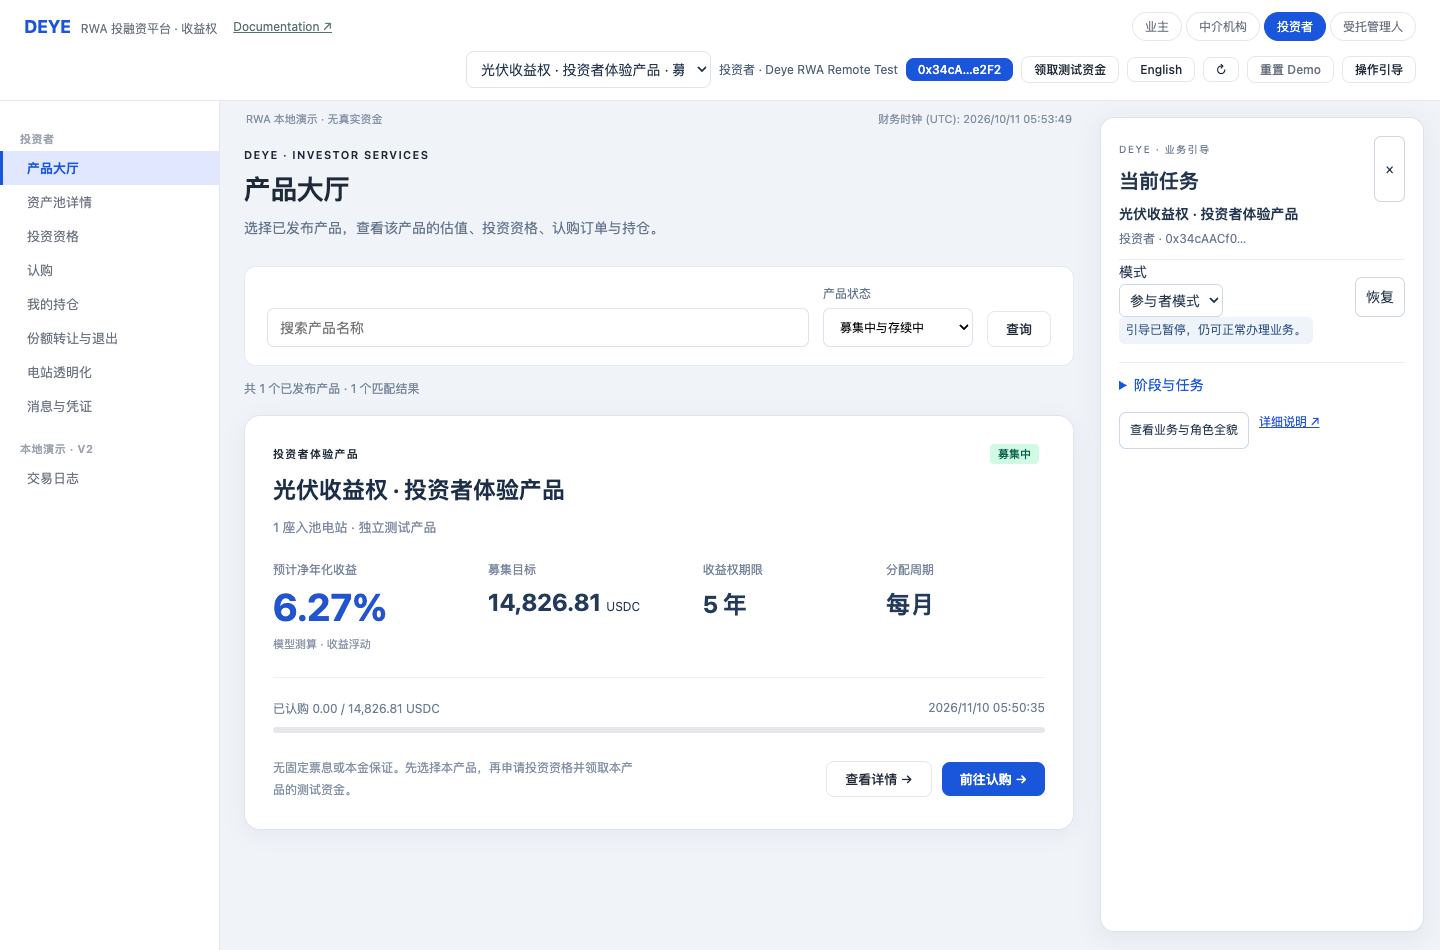
\includegraphics[width=\linewidth,height=.60\textheight,keepaspectratio]{assets/remote-hall.zh.png}\par 当前公网产品大厅。选定产品后，点击卡片右下角的认购入口。\end{center}
\end{landscape}
\clearpage\begin{landscape}
\subsection{D2 阅读投资者现金流时间轴}
本步由投资者操作。进入“资产池详情”后，按期查看业主付款、售电收入、回款延迟、池费用、保护储备及月度分配。

操作成功后，理解初始认购支出、期间分配和剩余资产价值是不同指标。下一步，投资者申请资格。

图中预计净年化收益是现金流IRR，并非合同票息。收益权期限结束后不附带设备残值，也不保证返还原始本金。

\begin{center}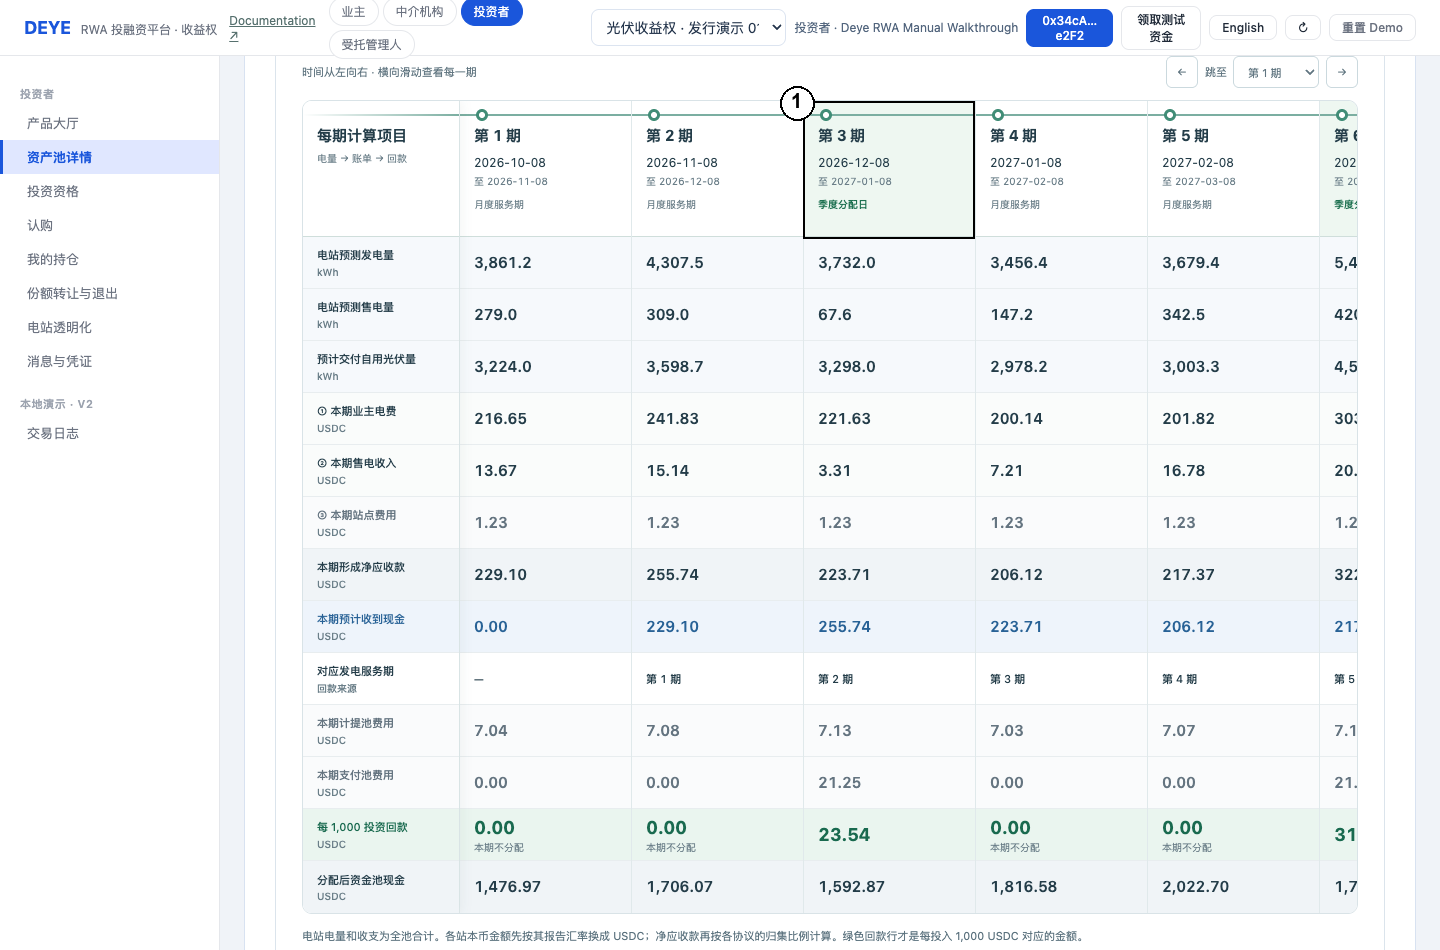
\includegraphics[width=\linewidth,height=.60\textheight,keepaspectratio]{assets/18-investor-timeline.png}\par 编号标出操作位置。插图来自隔离演练，金额和状态以当前产品为准。\end{center}
\end{landscape}
\clearpage\begin{landscape}
\subsection{D3 提交投资资格申请}
本步由投资者操作。进入“投资资格”后，阅读风险声明，勾选确认后点击编号1提交。

操作成功后，资格申请显示等待中介审批。下一步，中介机构审核该投资者。

专用预审账户可能已通过当前体验产品的资格。本次新发行产品仍需要按实际状态检查。

\begin{center}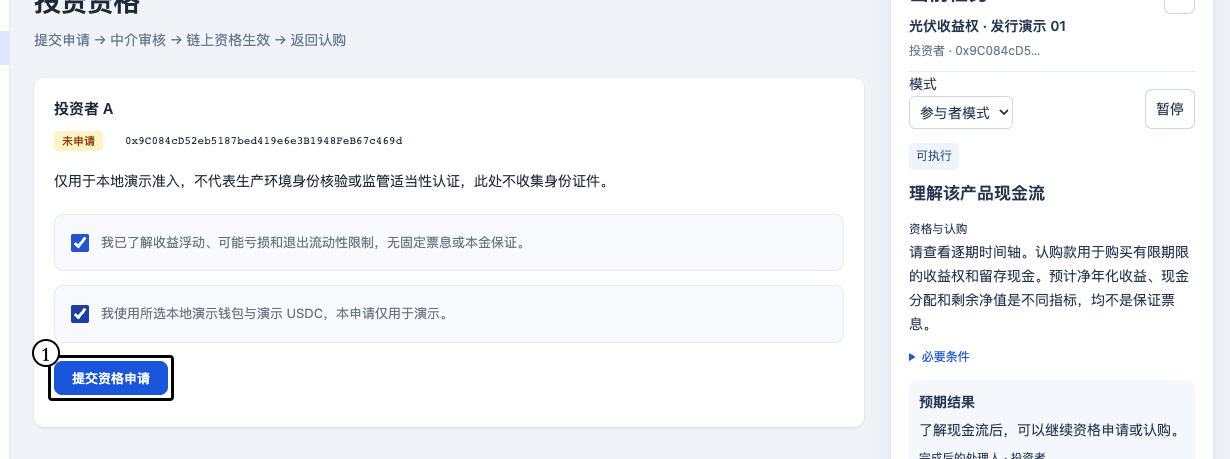
\includegraphics[width=\linewidth,height=.37\textheight,keepaspectratio]{assets/13-investor-apply-eligibility.zh-context.png}\par 编号1标出本步需要核对或提交的控件。\end{center}
\begin{center}
\includegraphics[width=.7\linewidth,height=1.55cm,keepaspectratio]{assets/13-investor-apply-eligibility.zh-detail.png}\end{center}
\end{landscape}
\clearpage\begin{landscape}
\subsection{D4 审核投资资格}
本步由中介机构操作。进入“投资者资格审核”后，按投资者地址打开申请，核对声明，选择通过并点击编号1签署资格登记交易。

操作成功后，该地址在本产品合约中获得资格。下一步，投资者领取资金并认购。

对投资者B重复本步。资格按产品分别记录，不是一个账户永久通过所有产品。

\begin{center}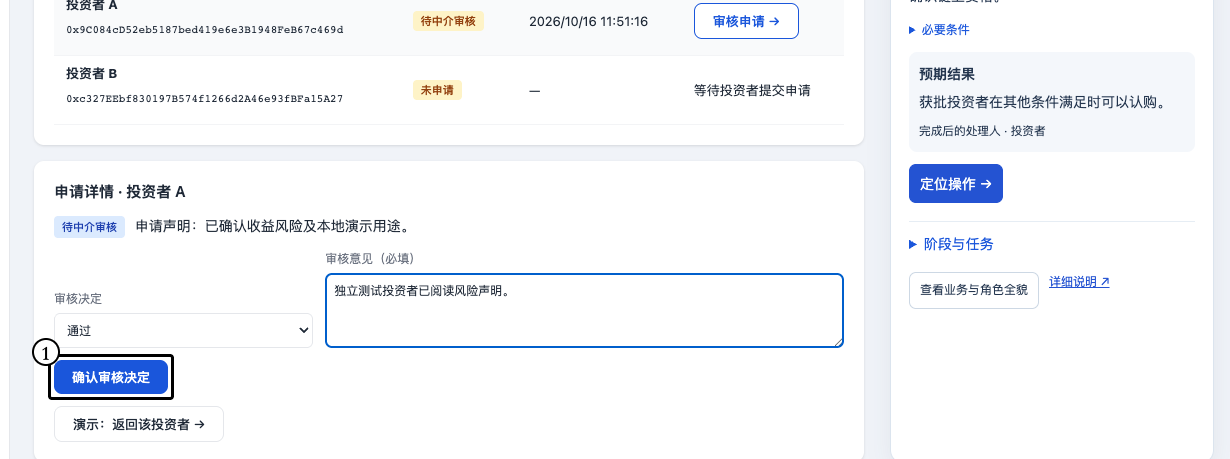
\includegraphics[width=\linewidth,height=.37\textheight,keepaspectratio]{assets/14-agent-eligible.zh-context.png}\par 编号1标出本步需要核对或提交的控件。\end{center}
\begin{center}
\includegraphics[width=.7\linewidth,height=1.55cm,keepaspectratio]{assets/14-agent-eligible.zh-detail.png}\end{center}
\end{landscape}
\clearpage\begin{landscape}
\subsection{D5 授权USDC并认购}
本步由投资者A操作。进入“认购”后，先领取当前产品的测试资金并检查余额，填写金额，再点击编号1。按钱包顺序确认USDC授权和认购交易。 在募集尚未结束且额度足够时，可以使用“继续追加认购”再次下单。每次只支付本次新增金额，系统累计托管款并要求中介重新审核最新总额。

操作成功后，认购款进入托管，订单显示金额和待中介审核状态，已发行份额暂为零。下一步，中介机构审核认购订单。

USDC授权只是允许合约扣款，第二笔认购交易成功才会形成托管订单。钱包拒签后应查看交易日志，不能把授权成功当作认购成功。

\begin{center}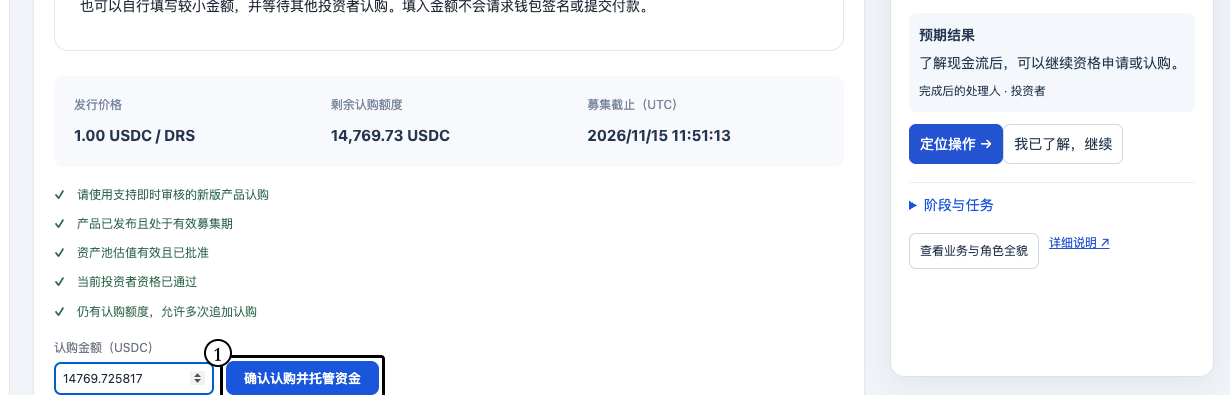
\includegraphics[width=\linewidth,height=.37\textheight,keepaspectratio]{assets/15-investor-subscribe.zh-context.png}\par 编号1标出本步需要核对或提交的控件。\end{center}
\begin{center}
\includegraphics[width=.7\linewidth,height=1.55cm,keepaspectratio]{assets/15-investor-subscribe.zh-detail.png}\end{center}
\end{landscape}
\clearpage\begin{landscape}
\subsection{D6 结算前取消认购}
本步由投资者A操作。进入该笔认购订单后，需要演示退款时，点击编号1退回本笔认购，并在钱包确认。

操作成功后，合约将全部托管金额退回原钱包，订单金额归零且不铸造份额。下一步，投资者可重新认购，或结束测试。

本产品的订单可由中介直接审核。成功结算前可以按页面条件全额取消，成功结算后不能再用认购退款取代转让或赎回。

\begin{center}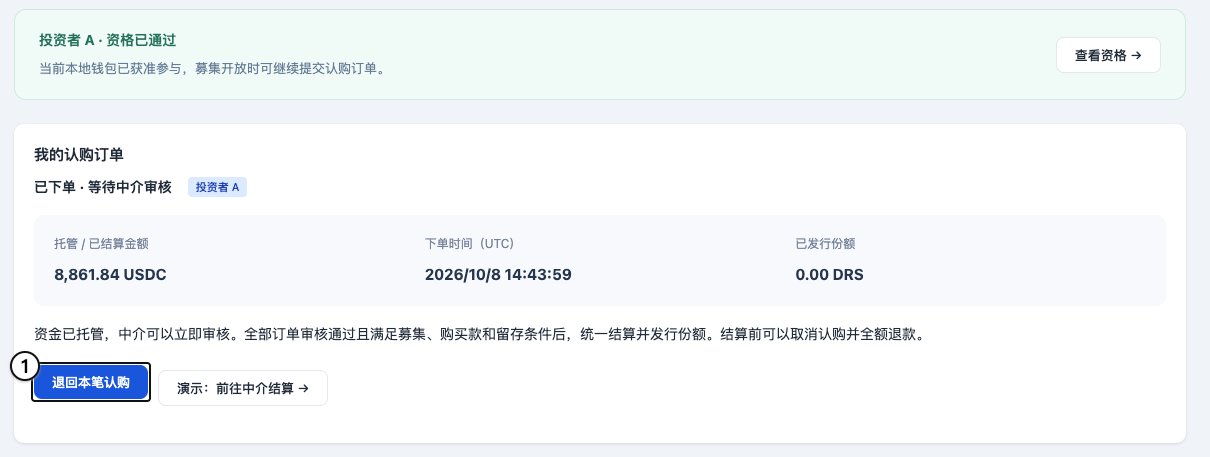
\includegraphics[width=\linewidth,height=.37\textheight,keepaspectratio]{assets/23-refund-context.png}\par 编号标出操作位置。插图来自隔离演练，金额和状态以当前产品为准。\end{center}
\begin{center}
\includegraphics[width=.7\linewidth,height=1.55cm,keepaspectratio]{assets/23-refund-detail.png}\end{center}
\end{landscape}
\clearpage\begin{landscape}
\subsection{D7 中介逐笔审核认购}
本步由中介机构操作。进入“产品运营”的认购审核列表后，按地址核对每笔订单、金额、资格和发行条款，选择通过并点击编号1。对投资者B也完成审核。

操作成功后，订单变为已审核通过，但DRS仍未铸造。下一步，中介机构执行统一发行结算。

拒绝会退回该笔订单的全部USDC。通过不会自动结算，也不需要推进时间。

\begin{center}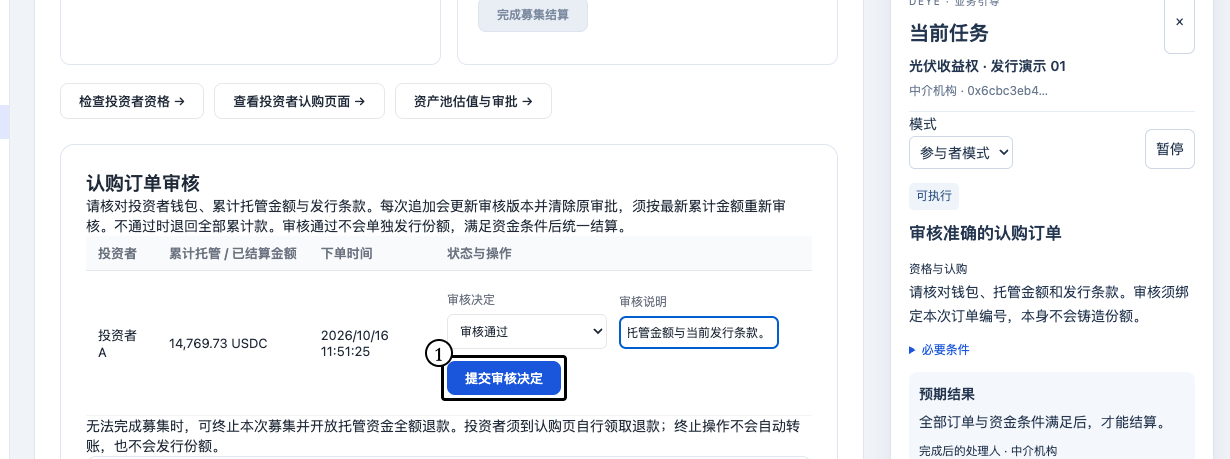
\includegraphics[width=\linewidth,height=.37\textheight,keepaspectratio]{assets/16-agent-review-subscription.zh-context.png}\par 编号1标出本步需要核对或提交的控件。\end{center}
\begin{center}
\includegraphics[width=.7\linewidth,height=1.55cm,keepaspectratio]{assets/16-agent-review-subscription.zh-detail.png}\end{center}
\end{landscape}
\clearpage\begin{landscape}
\subsection{D8 统一结算并发行DRS}
本步由中介机构操作。进入“产品运营”的发行与结算区后，确认所有待结算订单均通过审核，获批估值有效，资金足以购买全部收益权并保留10\%现金，再点击编号1结算。 10\%留存由结算合约自动完成，不需要另外存款。页面若提示尚缺资金，应请投资者按所示差额追加认购，再重新审核该累计订单。

操作成功后，合约向业主支付购买款，保留披露的现金并按认购金额铸造DRS。下一步，投资者查看持仓，中介开始运营。

募集达到目标70\%不是充分条件。如果70\%的资金仍不足以支付全部已签署购买价及初始留存，结算按钮仍不能使用。撤销募集是终止动作，不能用于审核通过。

\begin{center}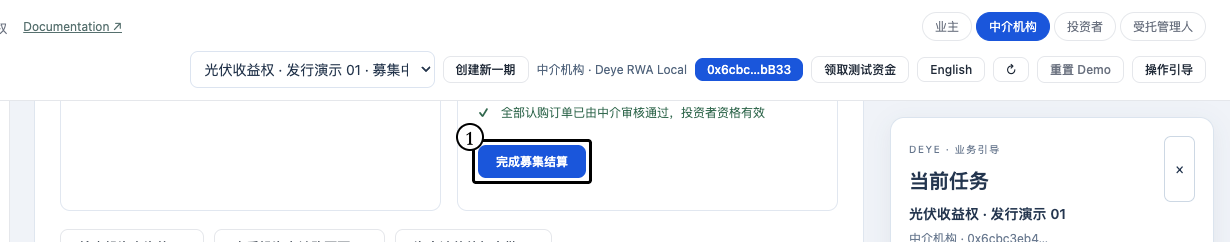
\includegraphics[width=\linewidth,height=.37\textheight,keepaspectratio]{assets/17-agent-settle.zh-context.png}\par 编号1标出本步需要核对或提交的控件。\end{center}
\begin{center}
\includegraphics[width=.7\linewidth,height=1.55cm,keepaspectratio]{assets/17-agent-settle.zh-detail.png}\end{center}
\end{landscape}
\clearpage\begin{landscape}
\subsection{D9 确认结算后的持仓}
本步由投资者A和B操作。进入“我的持仓”后，刷新并查看已发行DRS数量、认购支出、分配和剩余NAV。

操作成功后，DRS数量大于零，订单已结算，份额与实际认购比例对应。下一步，中介机构按月处理运营。

如果USDC已托管而DRS仍为零，应先检查产品和结算交易状态，不要再次认购同样金额。

\begin{center}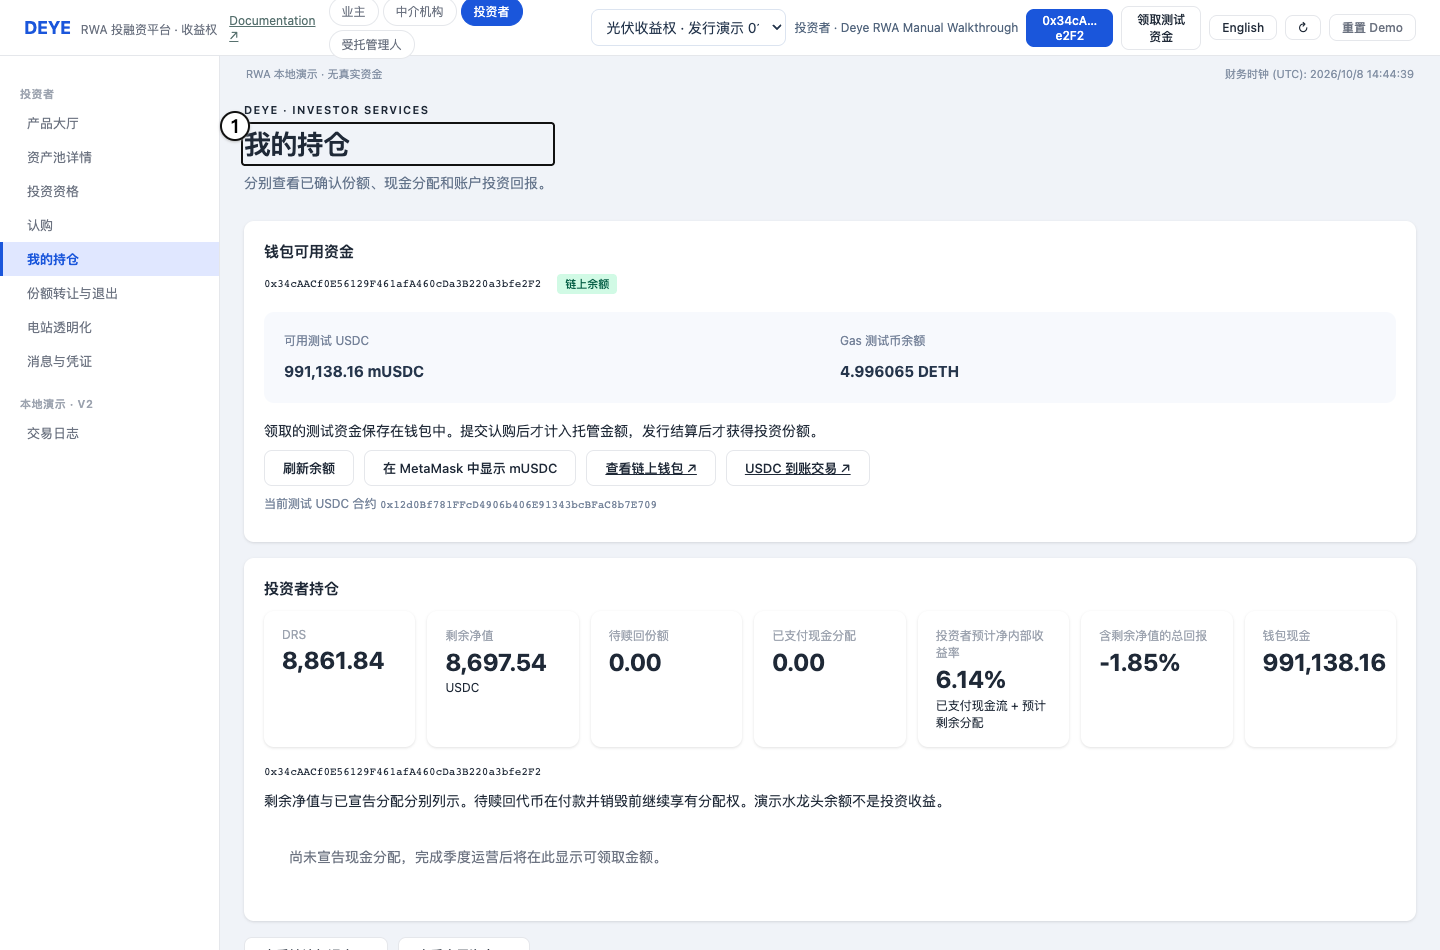
\includegraphics[width=\linewidth,height=.60\textheight,keepaspectratio]{assets/29-issued-position.png}\par 编号标出操作位置。插图来自隔离演练，金额和状态以当前产品为准。\end{center}
\end{landscape}
\clearpage\begin{landscape}
\section{月度回款、估值与分配}
\subsection{E1 推进一个演示财务月份}
本步由中介机构操作。进入“产品运营”的演示时间区后，点击右侧操作引导的“定位操作”。尚未到月度截止日时，选择弹窗提供的推进选项，阅读共享财务时钟提示并确认。该操作不会生成实时遥测，也不会自动批准净值或登记回款。

操作成功后，财务时间到达下一服务月末，电站采集时间保持不变。下一步，中介发布本期月度账单，再交由业主缴费。

推进时间影响整个测试链。多人测试时应先协调，不能为自己的一笔订单随意推进其他人的估值和期限。

\begin{center}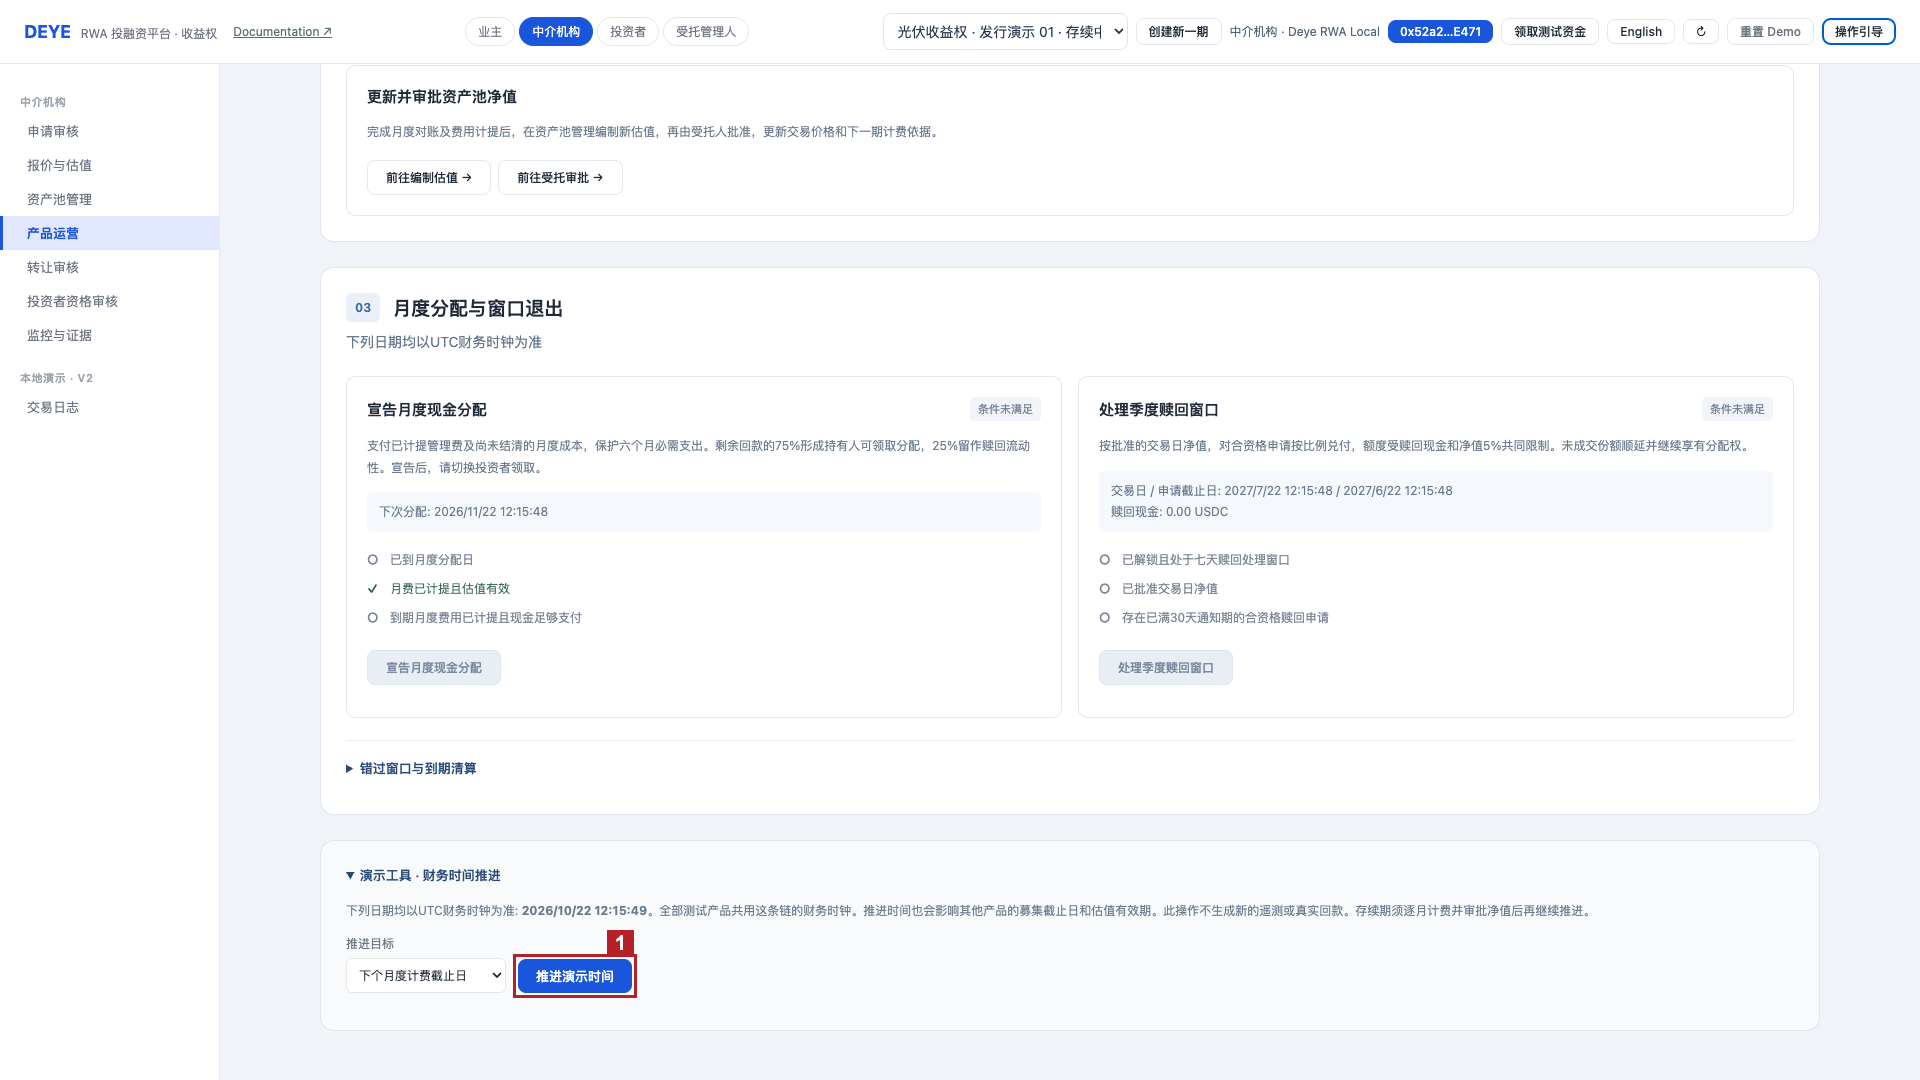
\includegraphics[width=\linewidth,height=.37\textheight,keepaspectratio]{assets/E1.zh-context.png}\par 编号1标出本期需要核对或签署的操作。截图来自隔离测试，金额和日期以当前产品为准。\end{center}
\begin{center}
\includegraphics[width=.7\linewidth,height=1.55cm,keepaspectratio]{assets/E1.zh-detail.png}\end{center}
\end{landscape}
\clearpage\begin{landscape}
\subsection{E2 发布月度缴费账单}
本步由中介机构操作。进入「监控与证据」的月度账单区后，核对服务期编号和已有的完整历史月份，检查本期业主电费、售电收入、成本及汇率，再点击编号1发布账单并确认钱包交易。

操作成功后，链上账单绑定本期业主地址、应付测试USDC金额和证据摘要，款项尚未到账。下一步，业主切换自己的钱包完成本期缴费。

同一服务期不能重复发布。历史月份是明确标记的计量示例，不是财务时钟所在月份的新遥测。

\begin{center}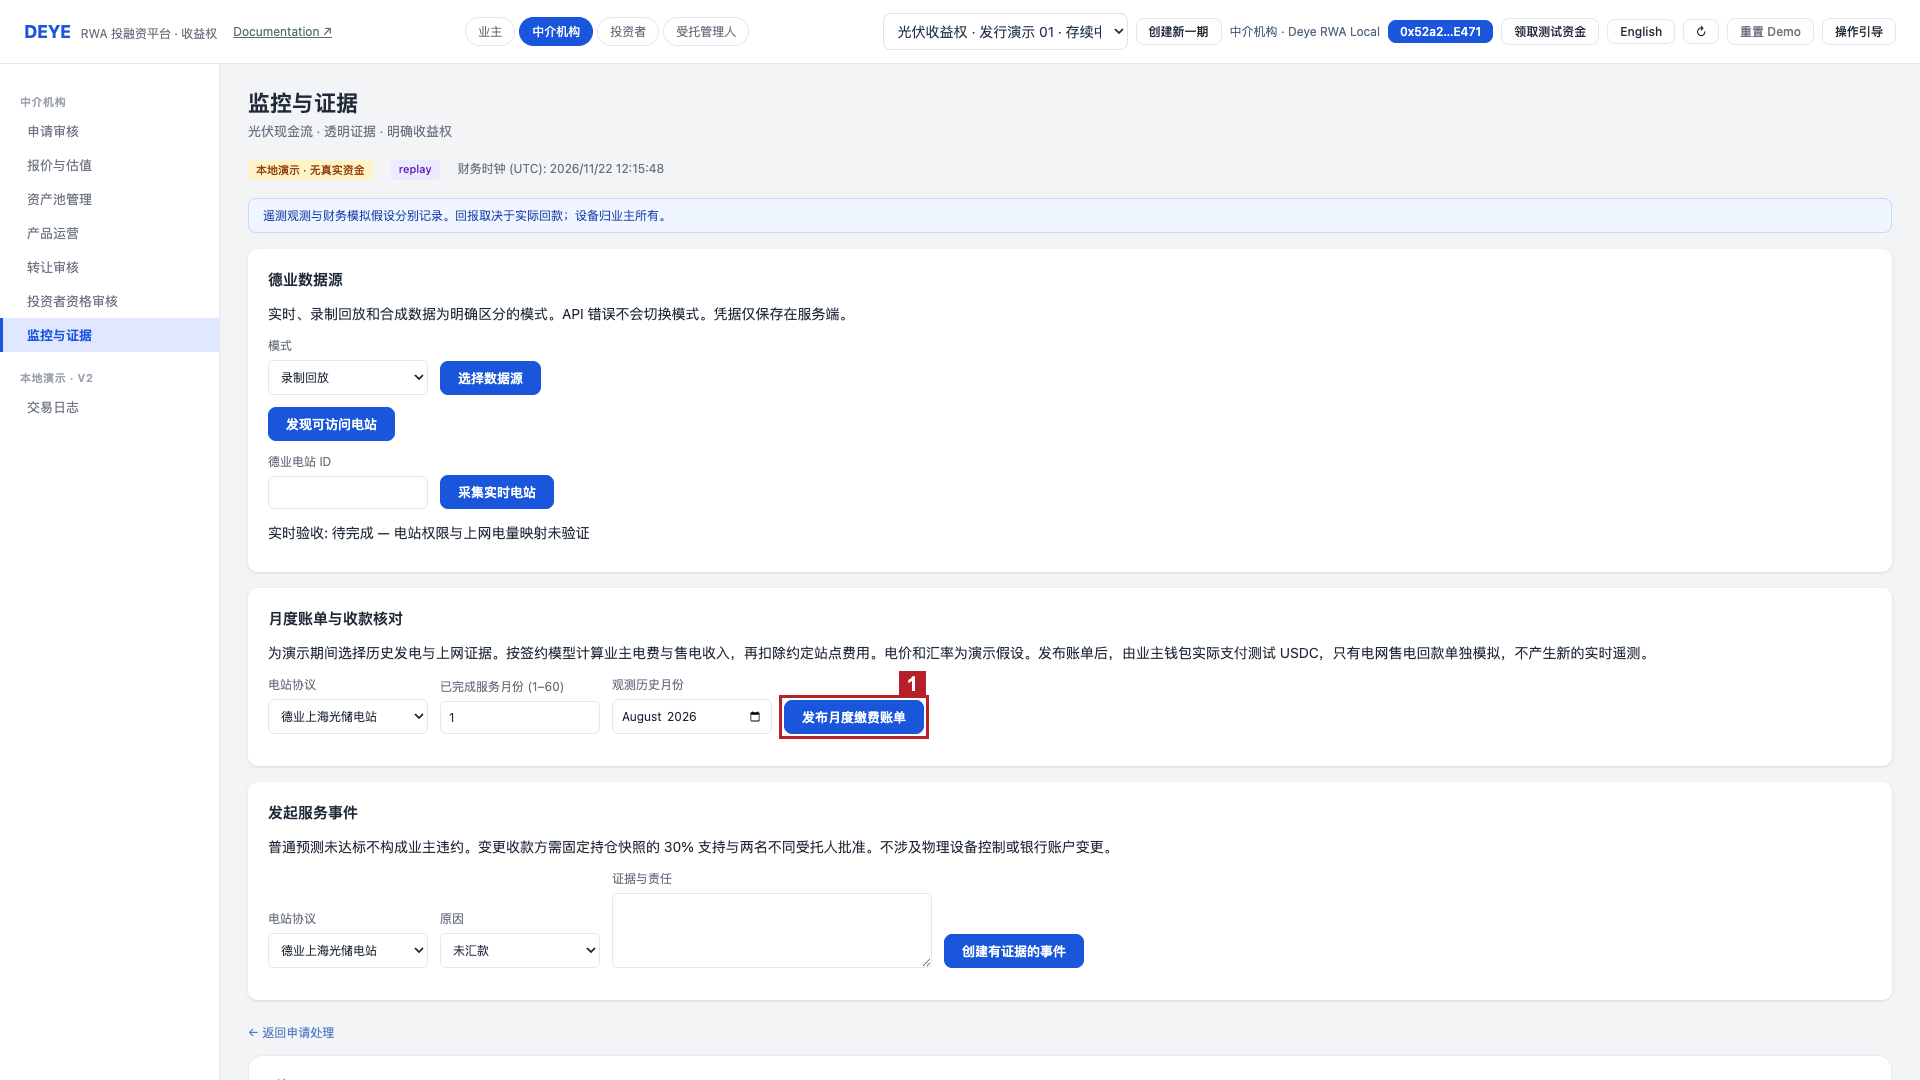
\includegraphics[width=\linewidth,height=.37\textheight,keepaspectratio]{assets/E2.zh-context.png}\par 编号1标出本期需要核对或签署的操作。截图来自隔离测试，金额和日期以当前产品为准。\end{center}
\begin{center}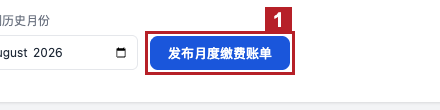
\includegraphics[width=.7\linewidth,height=1.55cm,keepaspectratio]{assets/E2.zh-detail.png}\end{center}
\end{landscape}
\clearpage\begin{landscape}
\subsection{E3 业主授权并支付月度电费}
本步由业主操作。进入「资金与月度缴费」的待付款账单后，核对产品、期数、币种和金额，点击编号1。先在钱包授权本张账单所需金额，再确认支付交易。余额不足时先领取测试资金。

操作成功后，本期电费从业主钱包转入账单合约，账单显示已付款并等待中介确认。下一步，中介登记单独的售电回款。

请勿向合约地址直接转账。普通USDC转账不等于指定账单已缴费，拒签和未确认交易也不算完成。

\begin{center}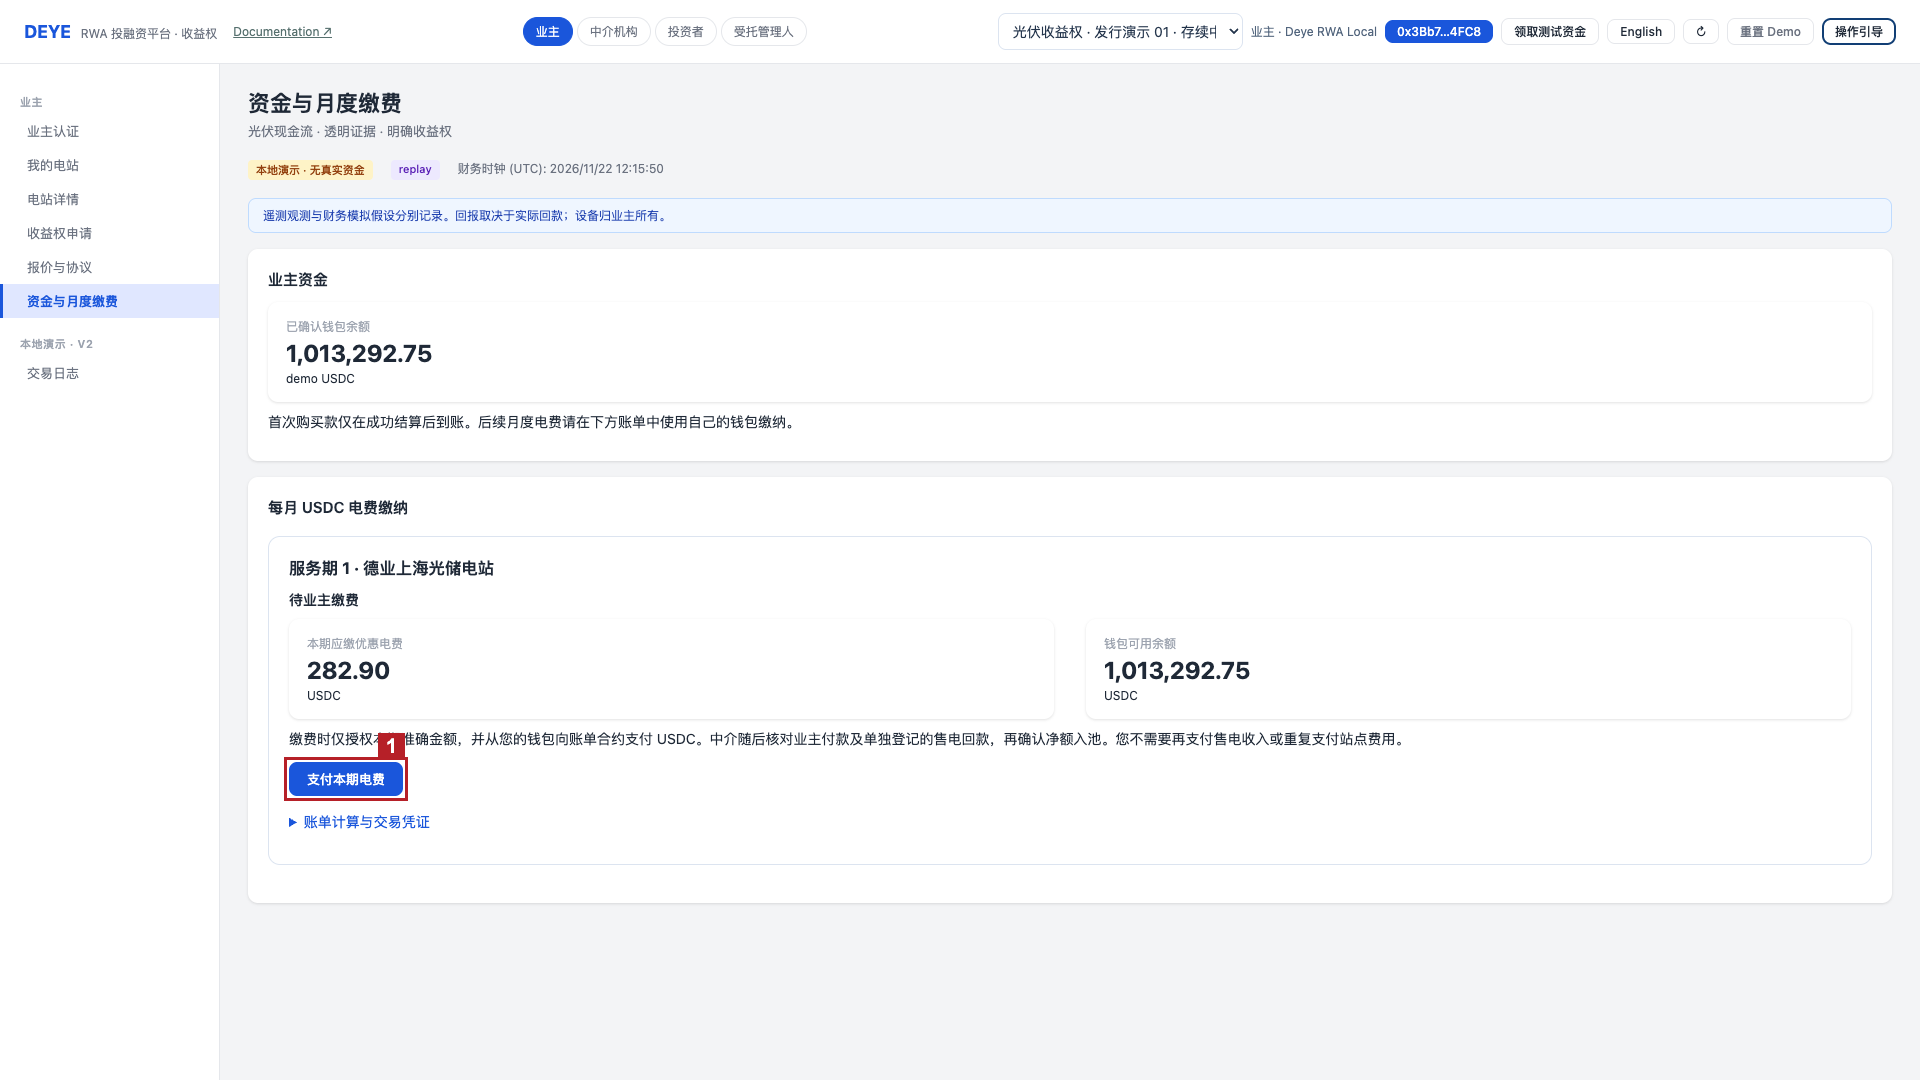
\includegraphics[width=\linewidth,height=.37\textheight,keepaspectratio]{assets/E3.zh-context.png}\par 编号1标出本期需要核对或签署的操作。截图来自隔离测试，金额和日期以当前产品为准。\end{center}
\begin{center}
\includegraphics[width=.7\linewidth,height=1.55cm,keepaspectratio]{assets/E3.zh-detail.png}\end{center}
\end{landscape}
\clearpage\begin{landscape}
\subsection{E3a 登记独立售电回款}
本步由中介机构操作。进入「监控与证据」的同一账单后，确认业主付款状态后，核对本期售电金额，点击编号1登记明确标注的模拟电网售电回款。

操作成功后，独立系统账户将本期售电部分转入账单合约，不替代业主的电费支付。下一步，中介核对两笔资金并确认入池。

只有这一部分回款仍为模拟。业主电费由业主本人钱包支付，不能由中介自动补足。

\begin{center}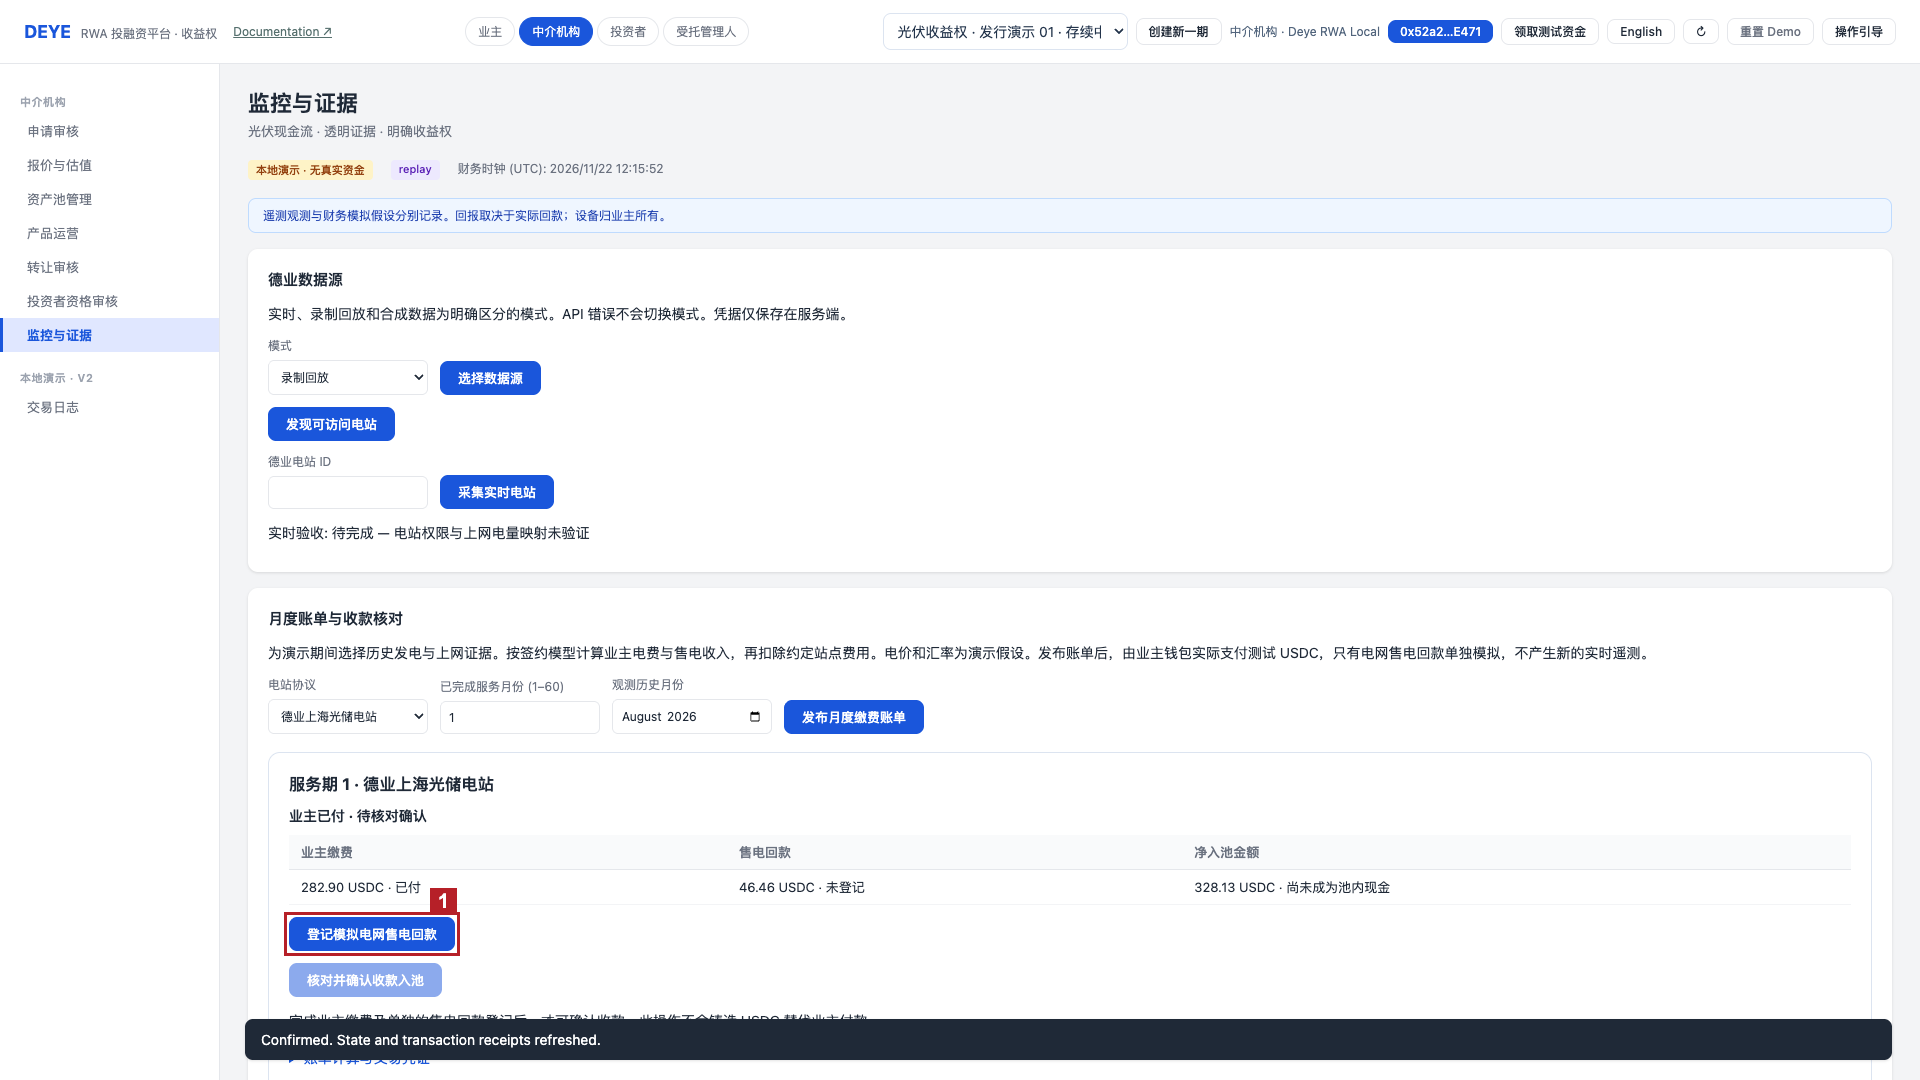
\includegraphics[width=\linewidth,height=.37\textheight,keepaspectratio]{assets/E3a.zh-context.png}\par 编号1标出本期需要核对或签署的操作。截图来自隔离测试，金额和日期以当前产品为准。\end{center}
\begin{center}
\includegraphics[width=.7\linewidth,height=1.55cm,keepaspectratio]{assets/E3a.zh-detail.png}\end{center}
\end{landscape}
\clearpage\begin{landscape}
\subsection{E3b 核对并确认收款入池}
本步由中介机构操作。进入「监控与证据」的同一账单后，核对业主付款、售电回款、站点费用及净额，点击编号1「核对并确认收款入池」，再在中介钱包确认交易。

操作成功后，合约一次性扣付站点费用，将约定净额转入资产池，并清除对应应收款。下一步，中介计提月度费用，再提交估值供受托审批。

确认前款项保存在账单合约，不计作资产池已收现金。完成后不能再次确认，也不会向已确认的旧账期重复收费。

\begin{center}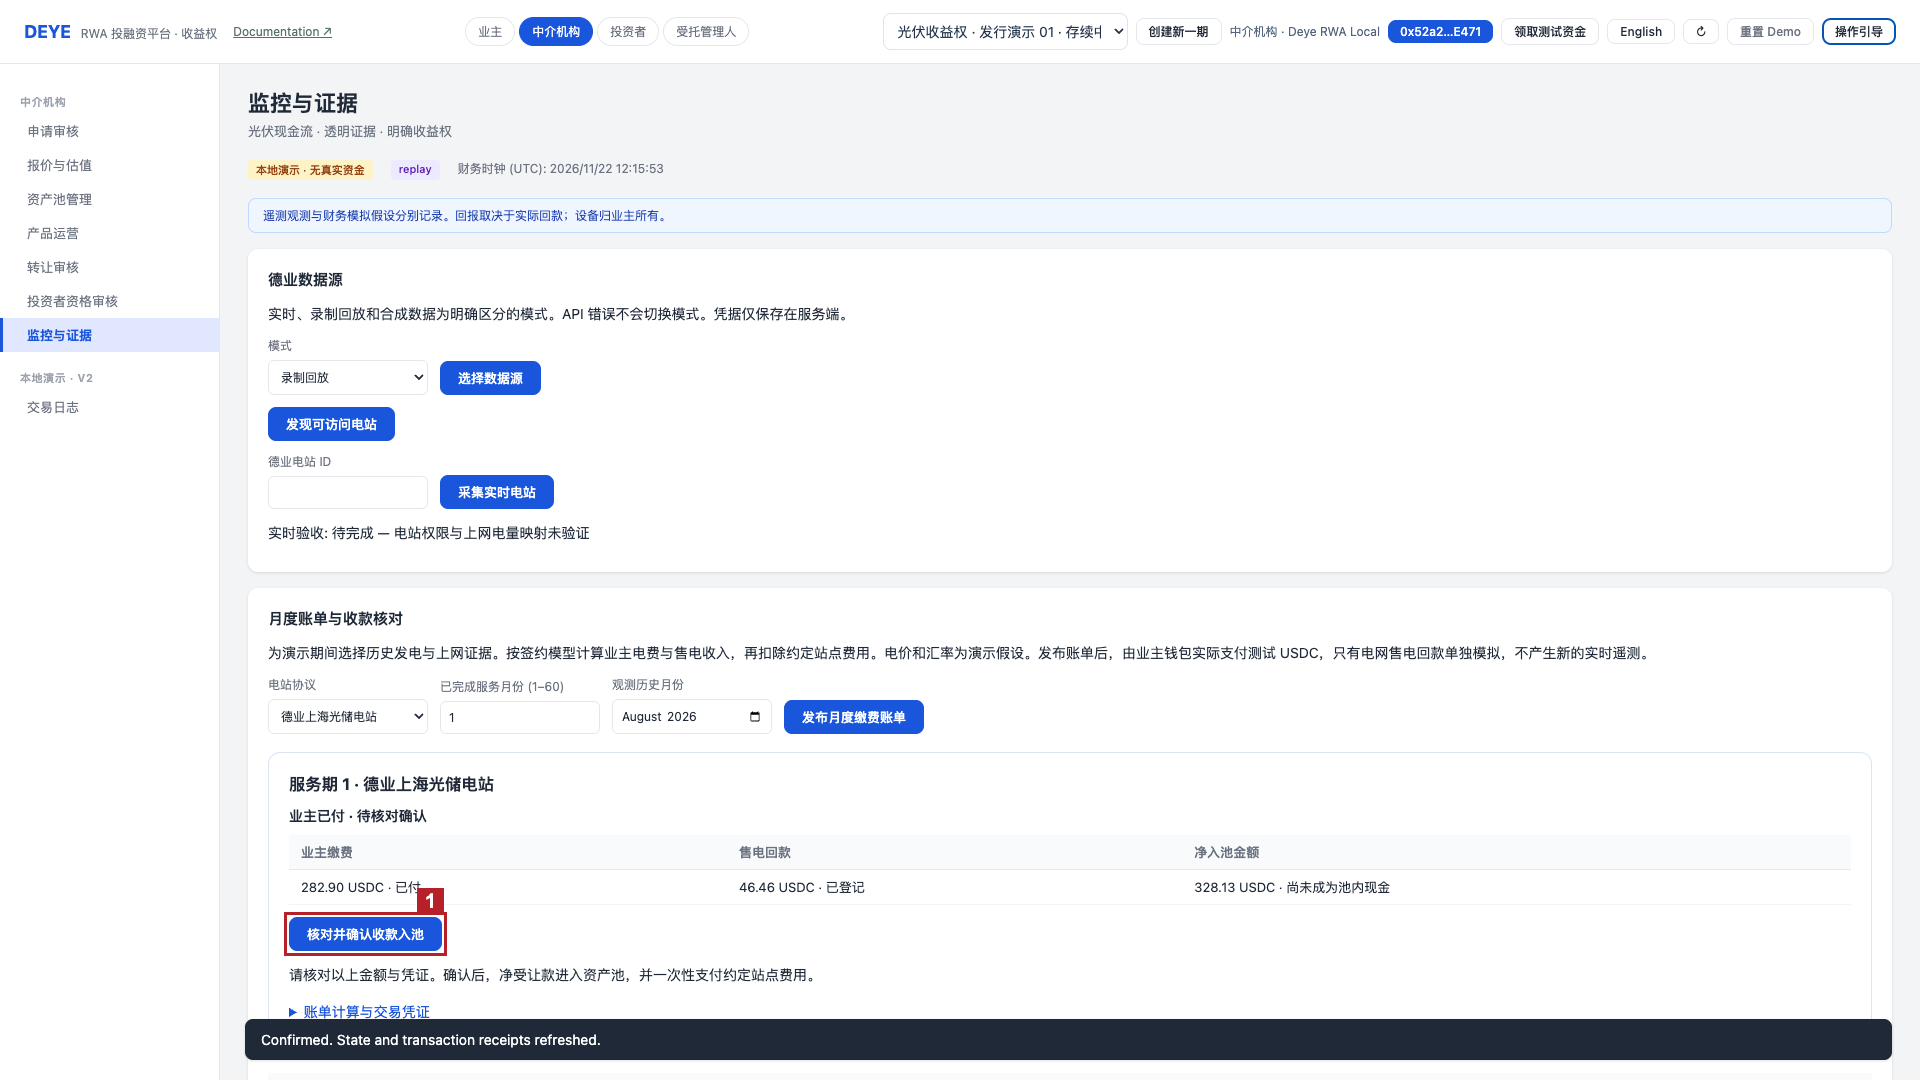
\includegraphics[width=\linewidth,height=.37\textheight,keepaspectratio]{assets/E3b.zh-context.png}\par 编号1标出本期需要核对或签署的操作。截图来自隔离测试，金额和日期以当前产品为准。\end{center}
\begin{center}
\includegraphics[width=.7\linewidth,height=1.55cm,keepaspectratio]{assets/E3b.zh-detail.png}\end{center}
\end{landscape}
\clearpage\begin{landscape}
\subsection{E4 计提月度池费用}
本步由中介机构操作。进入“产品运营”的费用区后，点击编号1计提本期费用。

操作成功后，系统按上一个获批月末NAV计算当月池费用，同时记录约定固定费用。下一步，中介提交本期资产池估值并交受托审批。

合计年费为0.5\%，月费按前一期获批NAV乘0.5\%再除以12计算。计提形成负债，支付时只结清这笔负债，不重新扣一遍。

\begin{center}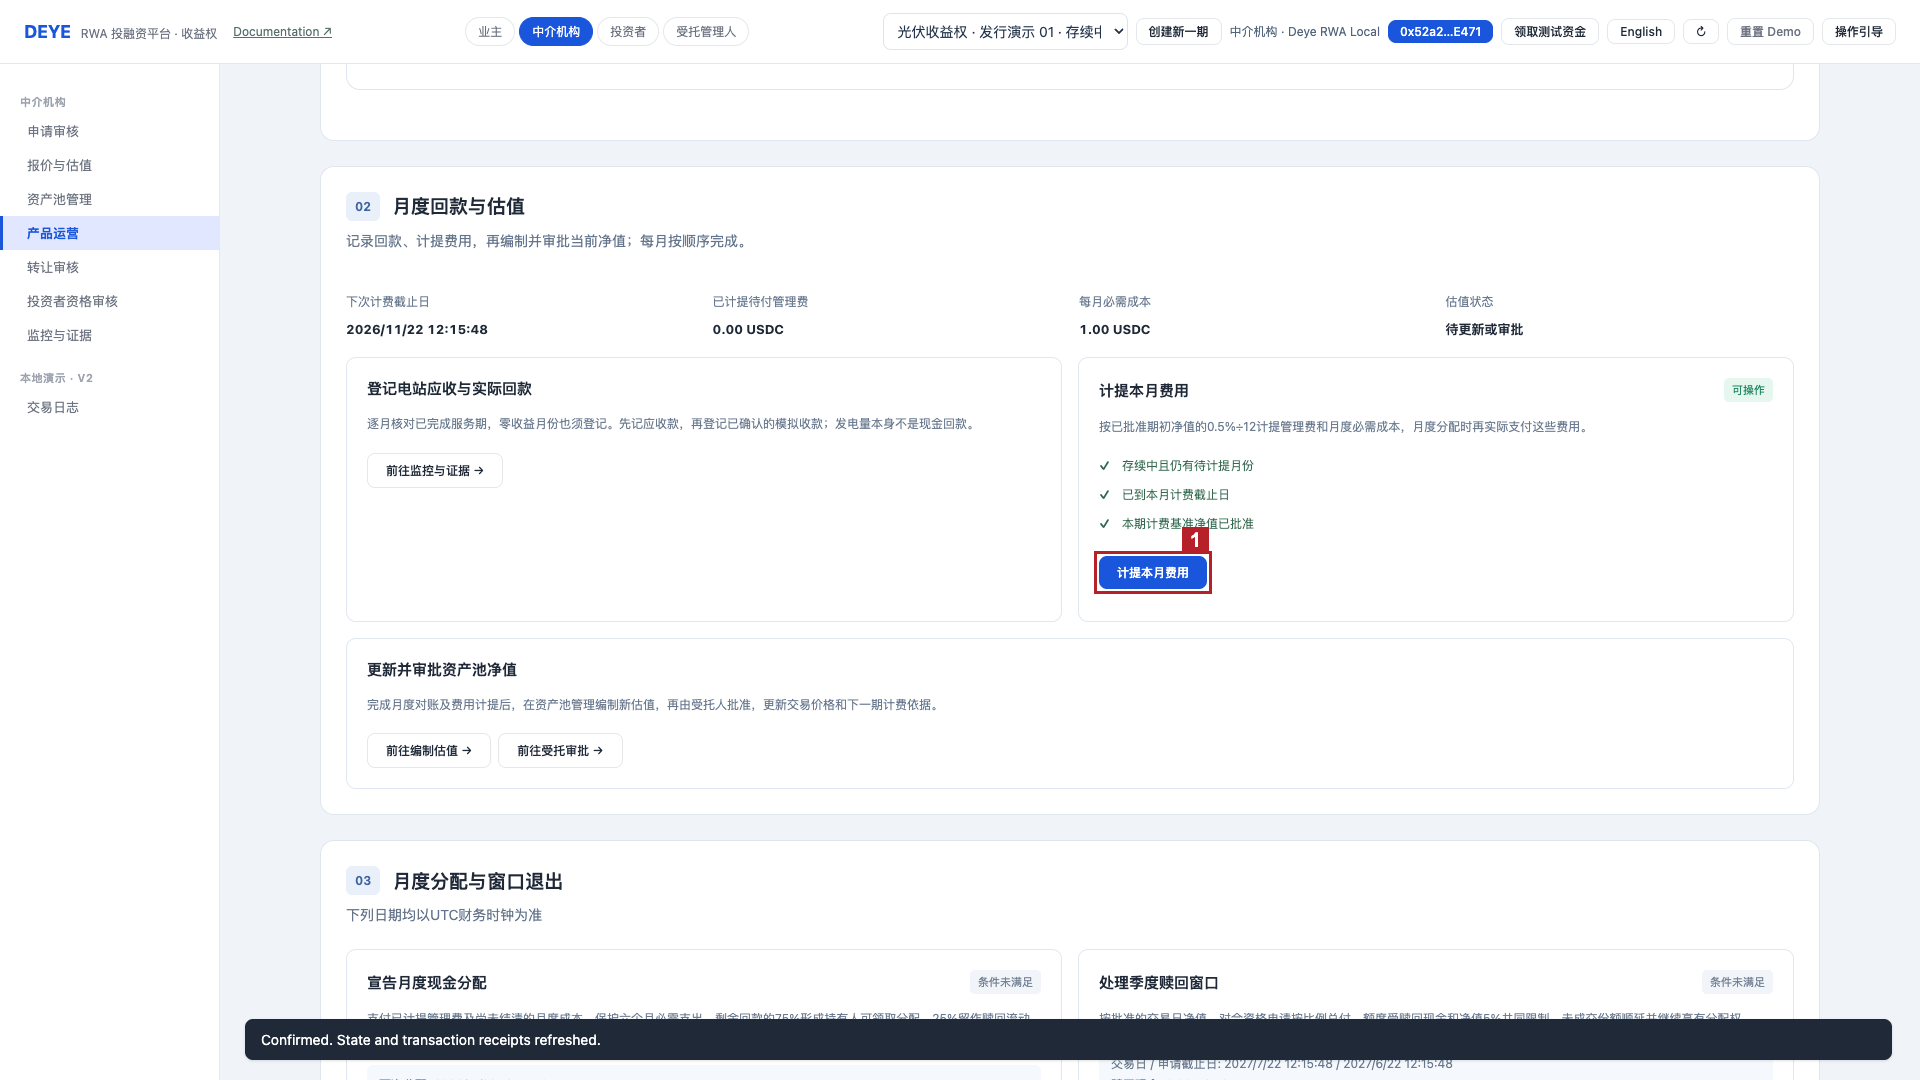
\includegraphics[width=\linewidth,height=.37\textheight,keepaspectratio]{assets/E4.zh-context.png}\par 编号1标出本期需要核对或签署的操作。截图来自隔离测试，金额和日期以当前产品为准。\end{center}
\begin{center}
\includegraphics[width=.7\linewidth,height=1.55cm,keepaspectratio]{assets/E4.zh-detail.png}\end{center}
\end{landscape}
\clearpage\begin{landscape}
\subsection{E5 更新运营后的净值}
本步由中介机构和受托管理人分别操作。进入“资产池管理”的估值区后，中介在回款登记和费用计提后编制本期估值，再交给受托管理人。受托人核对报告和假设，勾选已审核的确认项，再点击“批准并锚定估值”并在钱包确认。

操作成功后，本期估值获得链上批准，页面解除相应条件。下一步，中介返回产品运营宣告本月分配。

涉及转让、赎回或月度分配之前都需要有效估值。审批后发生重大资金动作，通常需要再次更新估值。

\begin{center}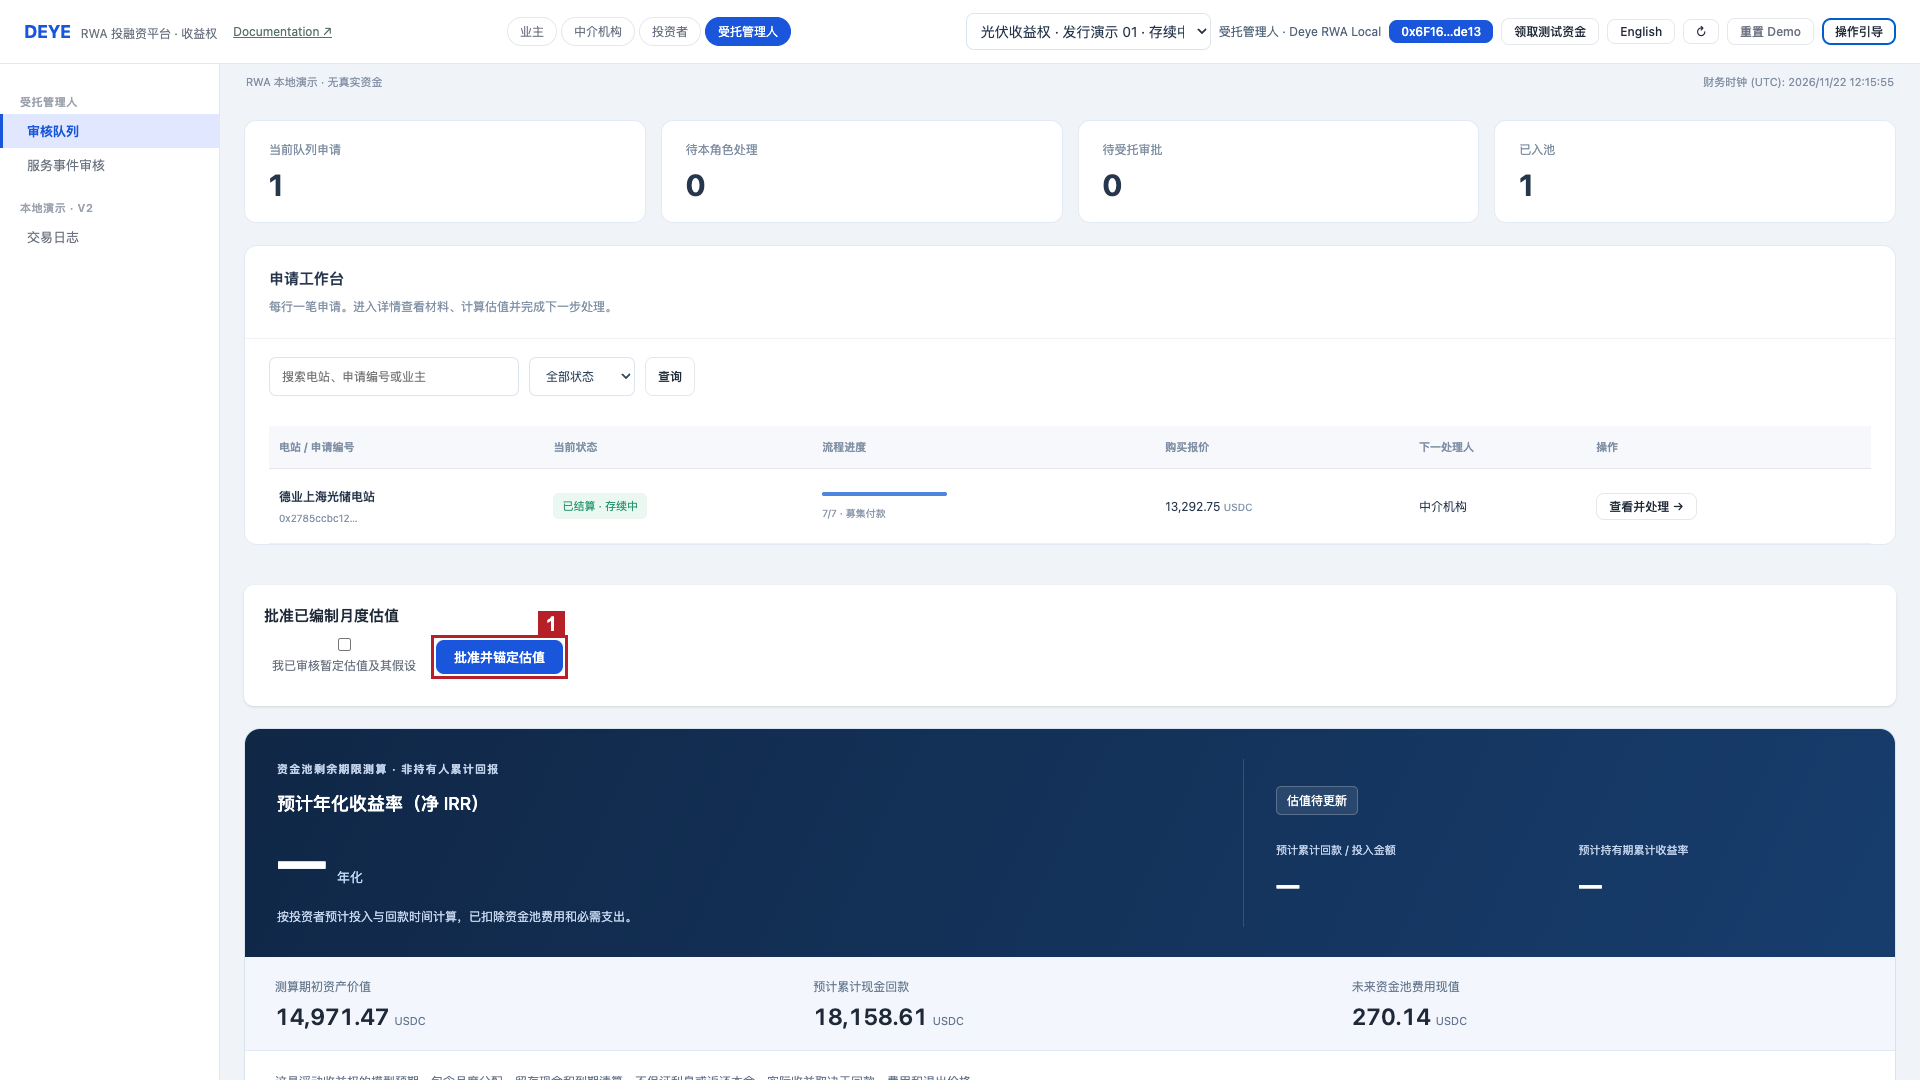
\includegraphics[width=\linewidth,height=.37\textheight,keepaspectratio]{assets/E5.zh-context.png}\par 编号1标出本期需要核对或签署的操作。截图来自隔离测试，金额和日期以当前产品为准。\end{center}
\begin{center}
\includegraphics[width=.7\linewidth,height=1.55cm,keepaspectratio]{assets/E5.zh-detail.png}\end{center}
\end{landscape}
\clearpage\begin{landscape}
\subsection{E6 月度结清费用并宣告分配}
本步由中介机构操作。进入“产品运营”的分配区后，确认本期回款、费用和估值已经核对并获受托批准后，点击编号1宣告月度分配。合约自动支付本期应付费用，恢复六个月必需费用储备，再将合格剩余回款的75\%形成领取权，25\%留作赎回流动性。

操作成功后，页面显示本次分配编号及各投资者的实际可领取金额。下一步，投资者通过交接入口进入“我的持仓”核对并领取。

每个月都可以按已到期的服务期处理一次。尚未批准估值时应先完成受托审批，已经领取完的旧分配不会替代本期审批任务。

\begin{center}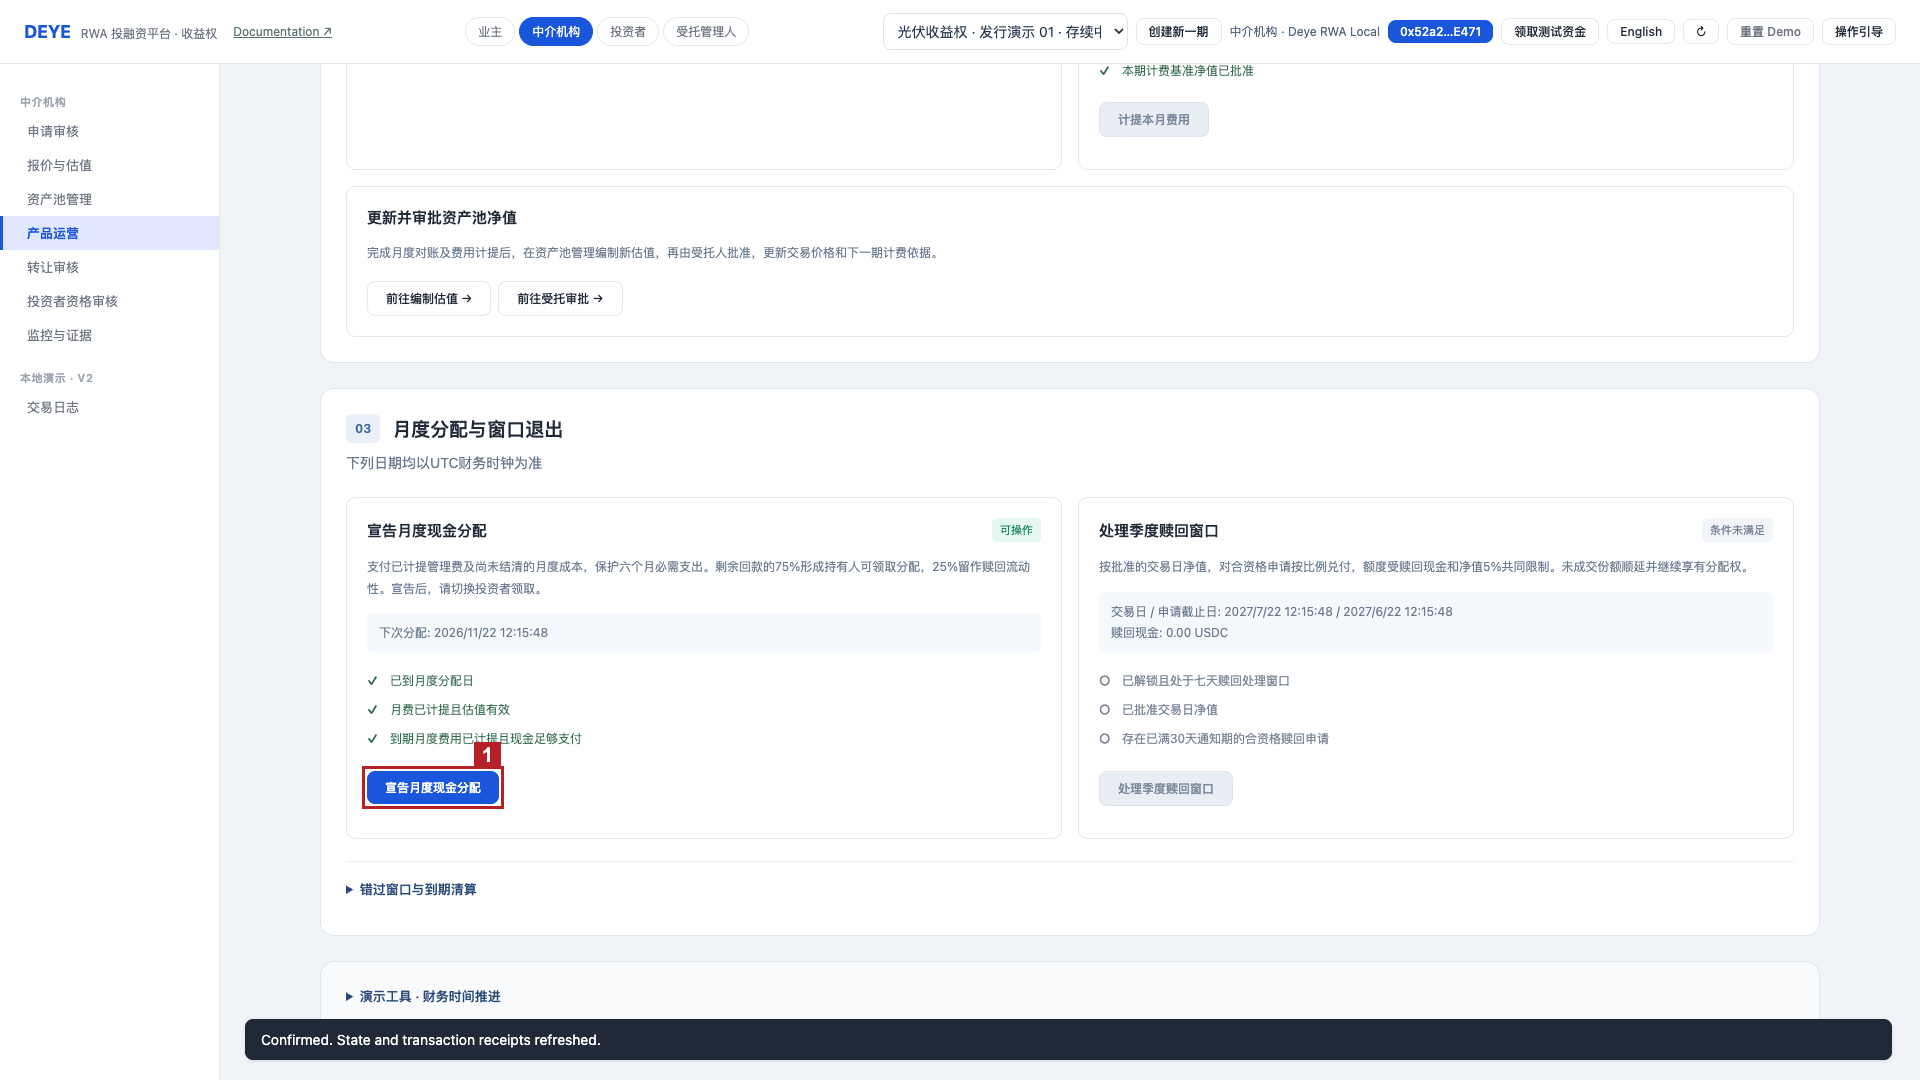
\includegraphics[width=\linewidth,height=.37\textheight,keepaspectratio]{assets/E6.zh-context.png}\par 编号1标出本期需要核对或签署的操作。截图来自隔离测试，金额和日期以当前产品为准。\end{center}
\begin{center}
\includegraphics[width=.7\linewidth,height=1.55cm,keepaspectratio]{assets/E6.zh-detail.png}\end{center}
\end{landscape}
\clearpage\begin{landscape}
\subsection{E7 领取已宣告的分配}
本步由投资者操作。进入“我的持仓”的分配记录后，按分配编号核对金额，点击编号1并签署领取交易。

操作成功后，USDC转入自己的钱包，该分配记录显示已领取。下一步，中介继续下一服务月，投资者按需要退出。

转让或赎回不应重复生成同一期领取权。仍在赎回托管中的未付款份额按规则保留分配权。

\begin{center}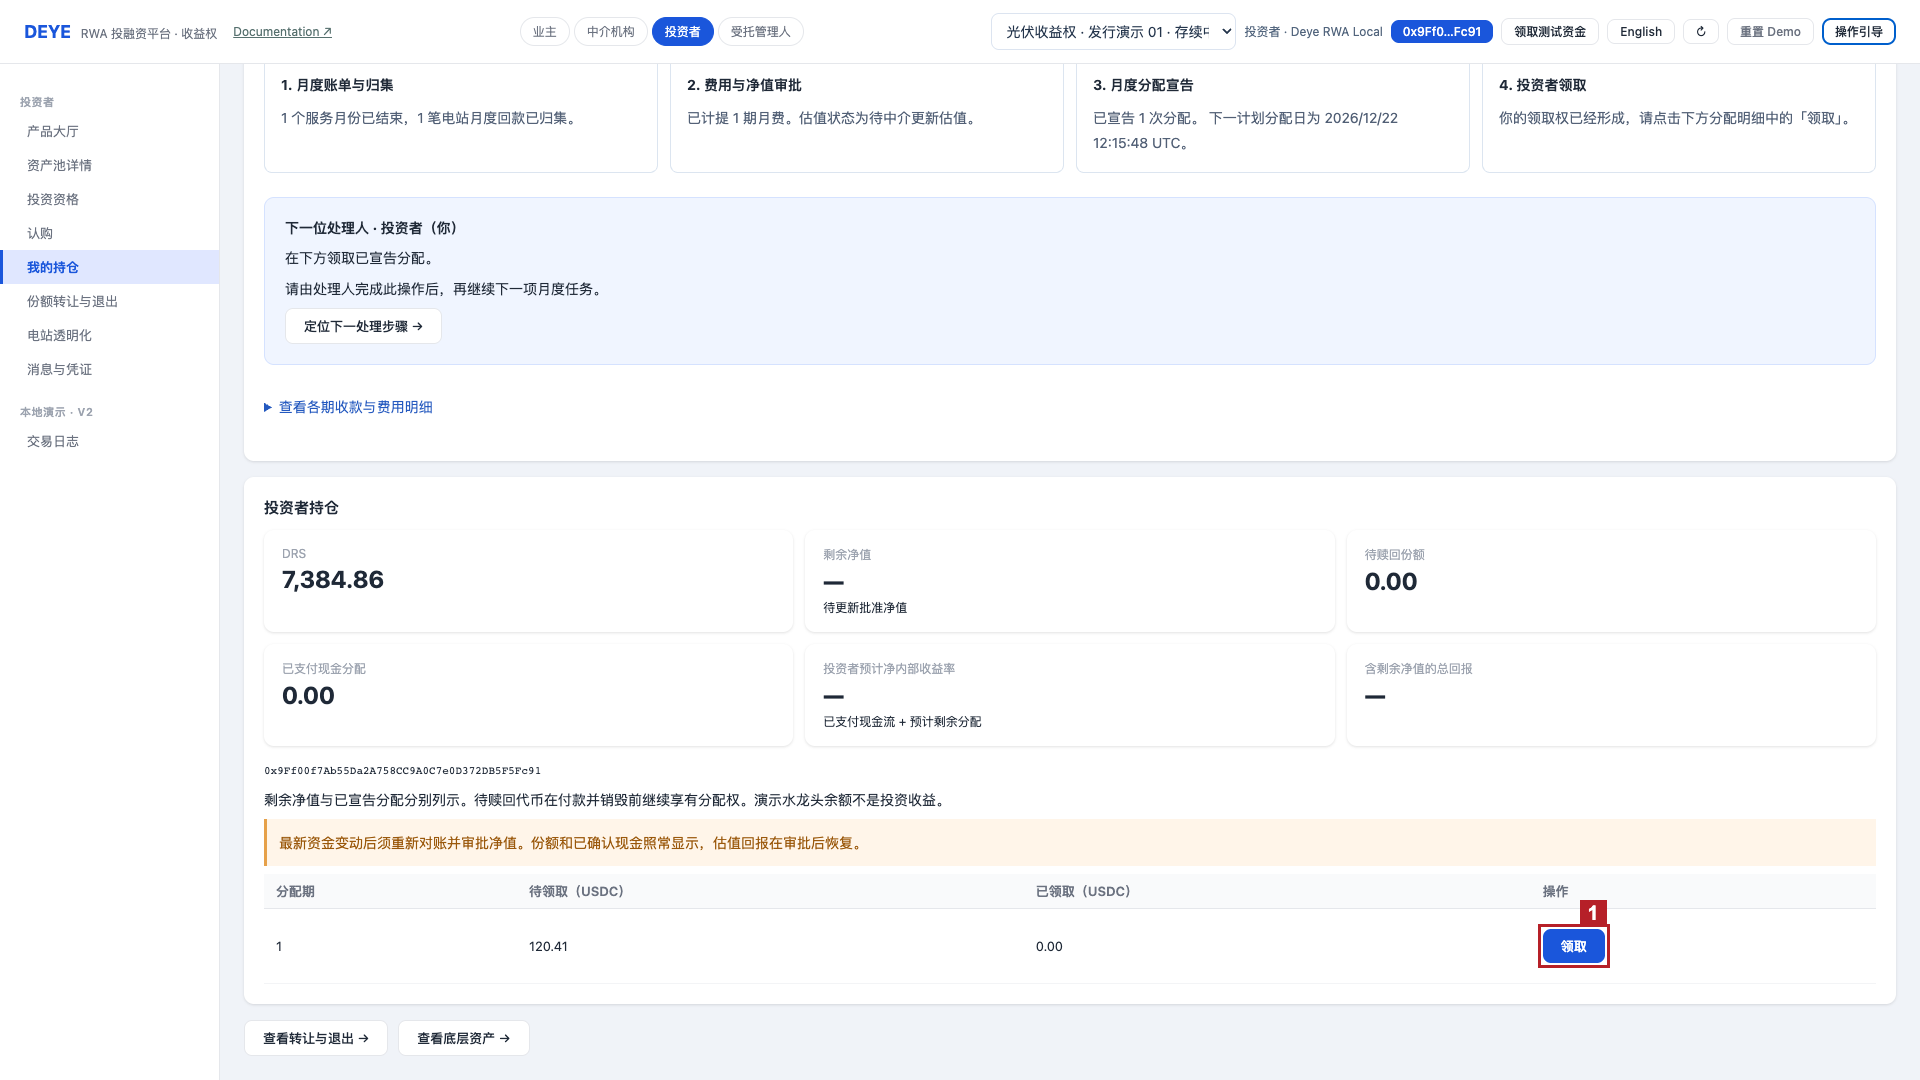
\includegraphics[width=\linewidth,height=.37\textheight,keepaspectratio]{assets/E7.zh-context.png}\par 编号1标出本期需要核对或签署的操作。截图来自隔离测试，金额和日期以当前产品为准。\end{center}
\begin{center}
\includegraphics[width=.7\linewidth,height=1.55cm,keepaspectratio]{assets/E7.zh-detail.png}\end{center}
\end{landscape}
\clearpage\begin{landscape}
\section{份额转让与季度赎回}
\subsection{F1 提出转让条款}
本步由投资者A作为卖方操作。进入“转让与赎回”后，选择已获资格的买方，填写份额与协商USDC总价，再点击编号1。

操作成功后，系统记录买卖双方、份额、价格及参考NAV。下一步，投资者B确认买方条款。

截图刻意使用偏离参考净值的价格，以展示中介复核。它不是平台推荐价格。

\begin{center}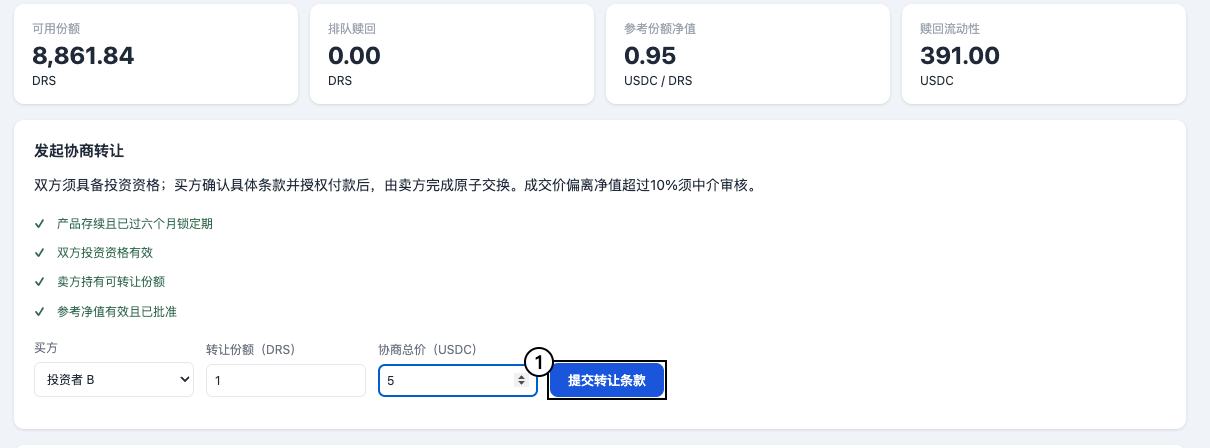
\includegraphics[width=\linewidth,height=.37\textheight,keepaspectratio]{assets/36-trade-context.png}\par 编号标出操作位置。插图来自隔离演练，金额和状态以当前产品为准。\end{center}
\begin{center}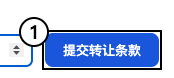
\includegraphics[width=.7\linewidth,height=1.55cm,keepaspectratio]{assets/36-trade-detail.png}\end{center}
\end{landscape}
\clearpage\begin{landscape}
\subsection{F2 买方同意并授权支付}
本步由投资者B操作。进入“转让与赎回”的待确认记录后，核对卖方地址、份额和总价，点击编号1并按钱包顺序授权USDC及确认条款。

操作成功后，合约记录买方对这组准确条款的同意。下一步，偏离超过10\%时由中介复核，否则由卖方结算。

对别的产品进行过USDC授权，不等于已授权当前产品。卖方不能代替买方同意。

\begin{center}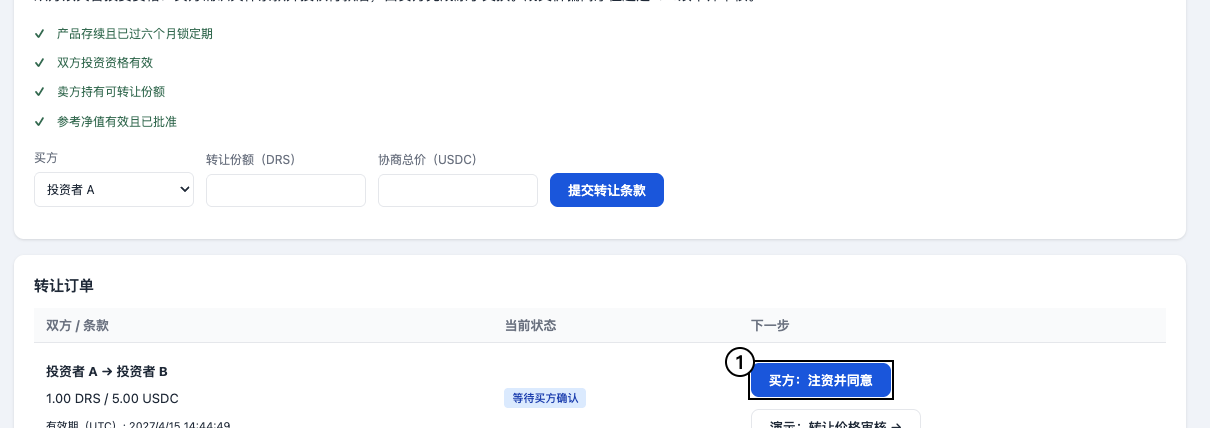
\includegraphics[width=\linewidth,height=.37\textheight,keepaspectratio]{assets/37-buyer-consent-context.png}\par 编号标出操作位置。插图来自隔离演练，金额和状态以当前产品为准。\end{center}
\begin{center}
\includegraphics[width=.7\linewidth,height=1.55cm,keepaspectratio]{assets/37-buyer-consent-detail.png}\end{center}
\end{landscape}
\clearpage\begin{landscape}
\subsection{F3 复核明显偏离NAV的转让}
本步由中介机构操作。进入“转让审核”后，核对协商价格及偏离比例，再点击编号1登记审批。

操作成功后，偏离超过10\%的转让满足额外审核条件。下一步，卖方执行原子结算。

批准不构成价格保证，也不会立即完成买卖双方付款和份额交付。

\begin{center}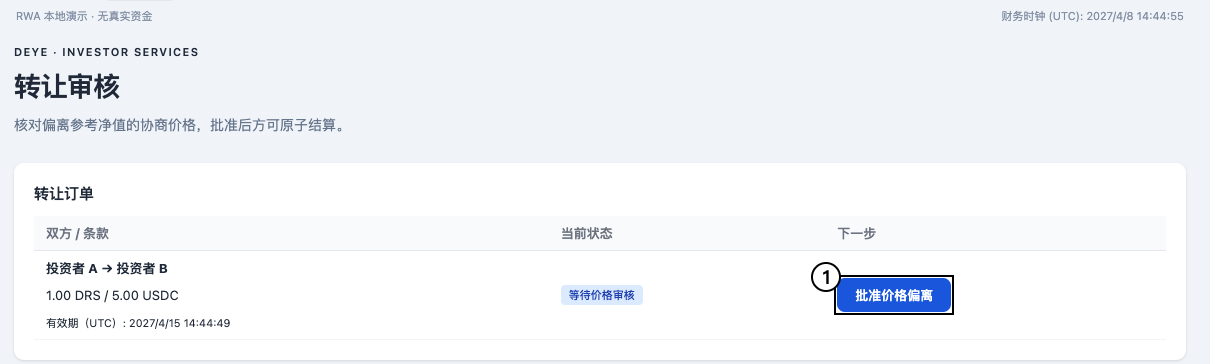
\includegraphics[width=\linewidth,height=.37\textheight,keepaspectratio]{assets/38-trade-review-context.png}\par 编号标出操作位置。插图来自隔离演练，金额和状态以当前产品为准。\end{center}
\begin{center}
\includegraphics[width=.7\linewidth,height=1.55cm,keepaspectratio]{assets/38-trade-review-detail.png}\end{center}
\end{landscape}
\clearpage\begin{landscape}
\subsection{F4 完成原子转让}
本步由投资者A作为卖方操作。进入“转让与赎回”的已同意记录后，确认买方同意、支付授权和所需审批齐备后，点击编号1。

操作成功后，同一交易内份额转给买方，USDC转给卖方。下一步，双方核对钱包余额与交易事件。

只有这一步成功才完成交易。应在Blockscout中同时核对份额和USDC两条转账。

\begin{center}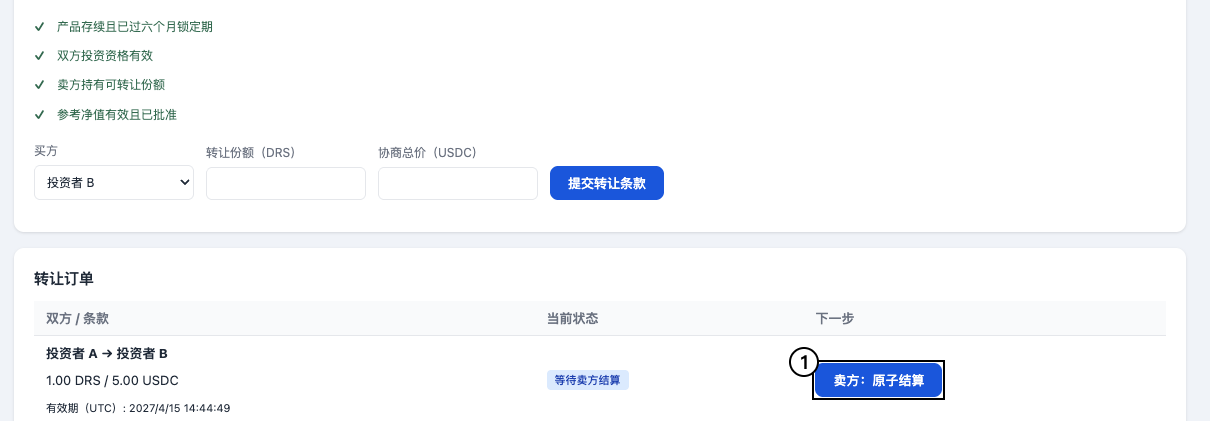
\includegraphics[width=\linewidth,height=.37\textheight,keepaspectratio]{assets/39-trade-settle-context.png}\par 编号标出操作位置。插图来自隔离演练，金额和状态以当前产品为准。\end{center}
\begin{center}
\includegraphics[width=.7\linewidth,height=1.55cm,keepaspectratio]{assets/39-trade-settle-detail.png}\end{center}
\end{landscape}
\clearpage\begin{landscape}
\subsection{F5 申请季度赎回}
本步由投资者A操作。进入“转让与赎回”的赎回区后，填写拟赎回份额，在截止前点击编号1。

操作成功后，请求份额进入托管，页面显示可处理日期与排队数量。下一步，中介在合格季度窗口处理。

申请时不是按当前参考价立即付款。实际成交按合格交易日的获批NAV，并排除已经宣告的分配。

\begin{center}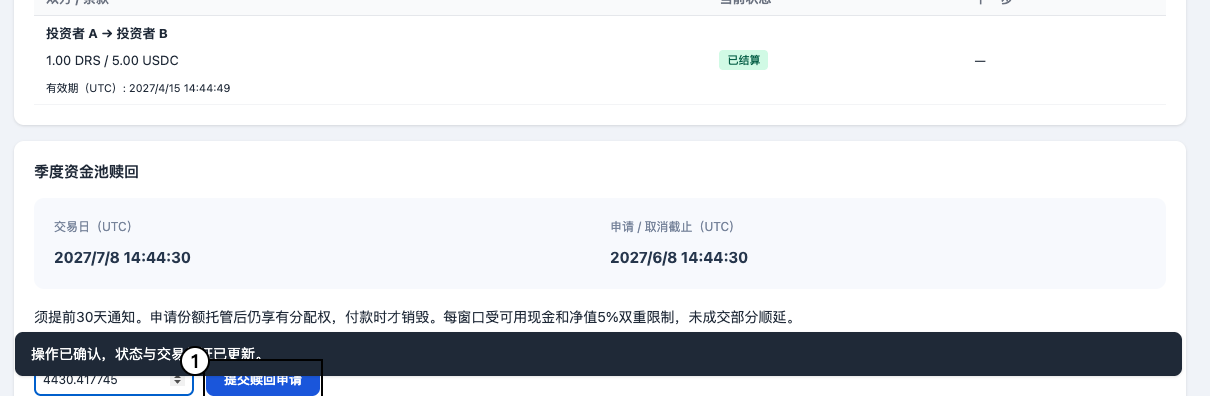
\includegraphics[width=\linewidth,height=.37\textheight,keepaspectratio]{assets/40-redemption-request-context.png}\par 编号标出操作位置。插图来自隔离演练，金额和状态以当前产品为准。\end{center}
\begin{center}
\includegraphics[width=.7\linewidth,height=1.55cm,keepaspectratio]{assets/40-redemption-request-detail.png}\end{center}
\end{landscape}
\clearpage\begin{landscape}
\subsection{F6 按窗口上限处理赎回}
本步由中介机构操作。进入“产品运营”的赎回窗口区后，在通知期和季度条件满足后更新并批准估值，再点击编号1处理。

操作成功后，合约按可用现金与5\%NAV上限计算成交比例，支付USDC并销毁已支付份额，余额继续排队。下一步，投资者查看已成交与剩余请求。

只成交一部分不是失败。必须分别核对支付金额、已销毁份额和未成交托管份额。

\begin{center}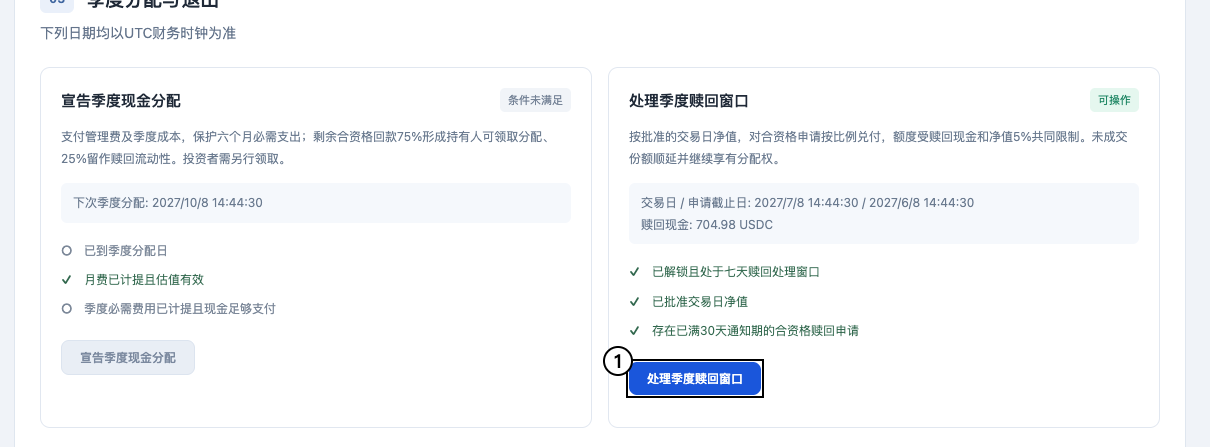
\includegraphics[width=\linewidth,height=.37\textheight,keepaspectratio]{assets/41-redemption-process-context.png}\par 编号标出操作位置。插图来自隔离演练，金额和状态以当前产品为准。\end{center}
\begin{center}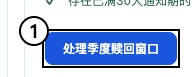
\includegraphics[width=.7\linewidth,height=1.55cm,keepaspectratio]{assets/41-redemption-process-detail.png}\end{center}
\end{landscape}
\clearpage\begin{landscape}
\subsection{F7 取消尚未成交的排队部分}
本步由投资者A操作。进入“转让与赎回”的剩余请求后，在下一截止前点击编号1取消未成交部分。

操作成功后，未支付份额退回钱包，已成交部分保持有效。下一步，投资者决定继续持有或重新申请。

本步不能撤销已经支付并销毁的成交部分。

\begin{center}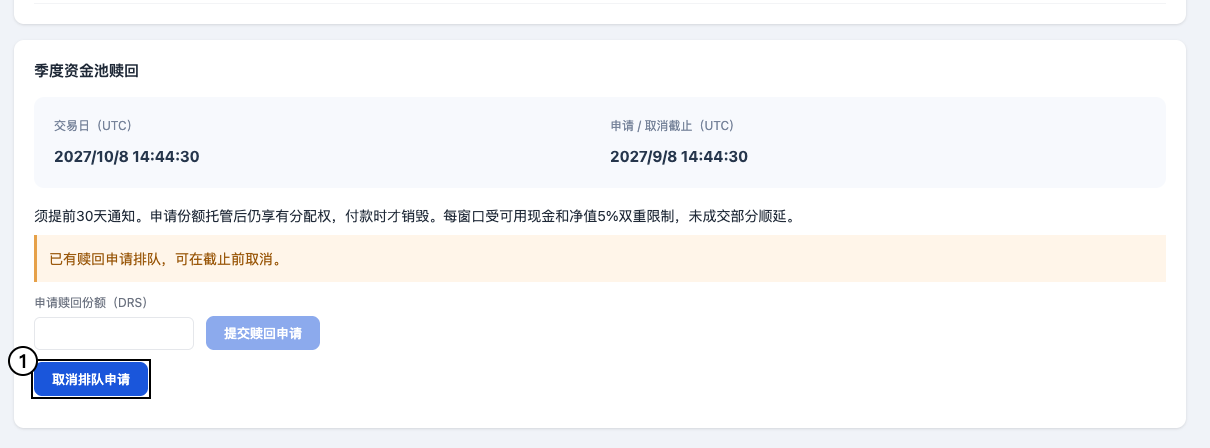
\includegraphics[width=\linewidth,height=.37\textheight,keepaspectratio]{assets/42-redemption-cancel-context.png}\par 编号标出操作位置。插图来自隔离演练，金额和状态以当前产品为准。\end{center}
\begin{center}
\includegraphics[width=.7\linewidth,height=1.55cm,keepaspectratio]{assets/42-redemption-cancel-detail.png}\end{center}
\end{landscape}
\clearpage\begin{landscape}
\section{服务事件与受托处置}
\subsection{G1 建立服务事件}
本步由中介机构操作。进入“电站监控”的服务事件区后，选择原因并写清事实、证据和拟处理事项，点击编号1。

操作成功后，系统记录事件，合约固定事件建立时的持仓快照。下一步，投资者按快照表示支持。

说明书使用明确标记的模拟回款事件，目的只是测试权限和处置条件。

\begin{center}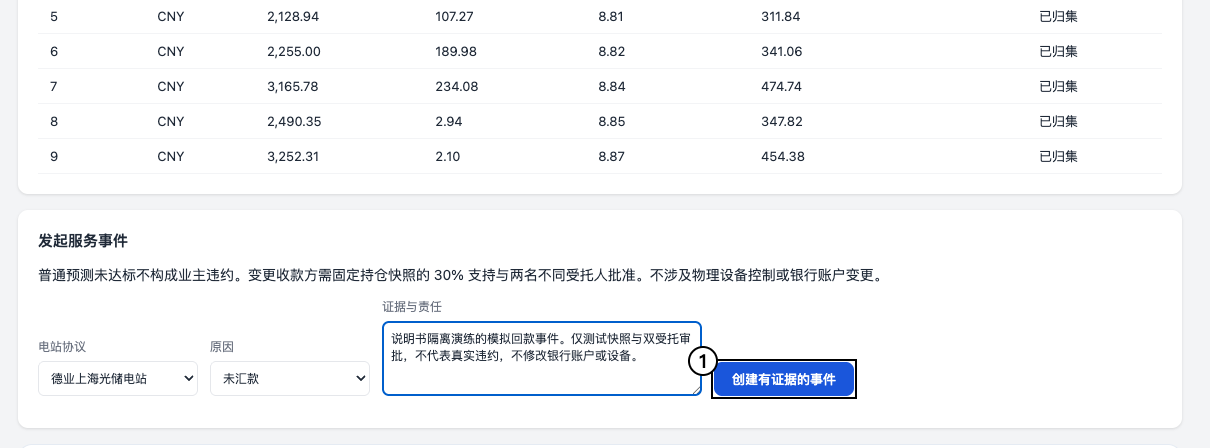
\includegraphics[width=\linewidth,height=.37\textheight,keepaspectratio]{assets/43-case-context.png}\par 编号标出操作位置。插图来自隔离演练，金额和状态以当前产品为准。\end{center}
\begin{center}
\includegraphics[width=.7\linewidth,height=1.55cm,keepaspectratio]{assets/43-case-detail.png}\end{center}
\end{landscape}
\clearpage\begin{landscape}
\subsection{G2 按固定快照支持处置}
本步由投资者A操作。进入“我的持仓”的服务事件记录后，阅读事件原因与拟变更收款方，点击编号1支持。

操作成功后，支持权重按事件快照计算，达到30\%后允许受托审批。下一步，受托管理人A独立审核。

后续转让不会重新生成快照权重，同一份额不能被重复计票。

\begin{center}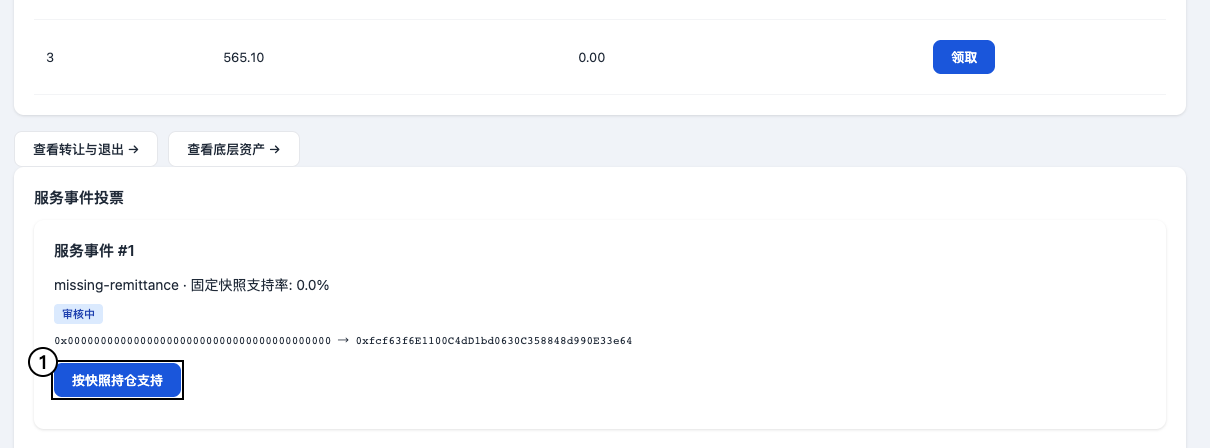
\includegraphics[width=\linewidth,height=.37\textheight,keepaspectratio]{assets/44-support-context.png}\par 编号标出操作位置。插图来自隔离演练，金额和状态以当前产品为准。\end{center}
\begin{center}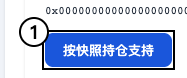
\includegraphics[width=.7\linewidth,height=1.55cm,keepaspectratio]{assets/44-support-detail.png}\end{center}
\end{landscape}
\clearpage\begin{landscape}
\subsection{G3 第一位受托人批准}
本步由受托管理人A操作。进入“受托处置”的事件详情后，核对快照比例、原因和收款地址，点击编号1。

操作成功后，合约记录第一位审批人的地址，但尚不完成变更。下一步，受托管理人B再次独立审核。

同一个受托地址不能重复点击来替代第二个人。

\begin{center}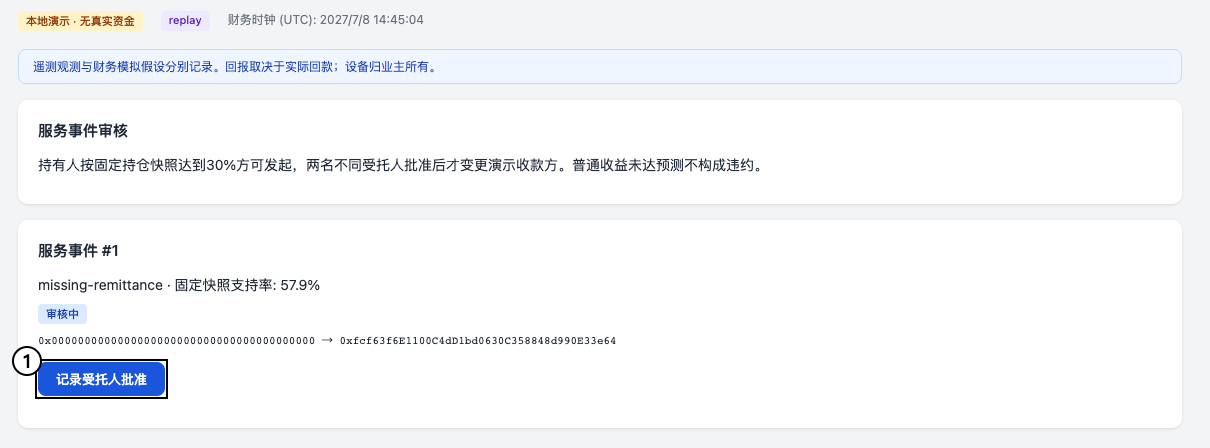
\includegraphics[width=\linewidth,height=.37\textheight,keepaspectratio]{assets/45-trustee-a-context.png}\par 编号标出操作位置。插图来自隔离演练，金额和状态以当前产品为准。\end{center}
\begin{center}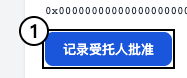
\includegraphics[width=.7\linewidth,height=1.55cm,keepaspectratio]{assets/45-trustee-a-detail.png}\end{center}
\end{landscape}
\clearpage\begin{landscape}
\subsection{G4 第二位受托人批准并执行}
本步由受托管理人B操作。进入同一事件详情后，切换到受托人B对应钱包并重新登录，独立核对后点击编号1。

操作成功后，合约核对两名不同审批人并执行演示收款方变更。下一步，中介核对执行结果并继续运营。

两位受托人都属于受托管理人角色。页面角色相同，但钱包地址必须不同。

\begin{center}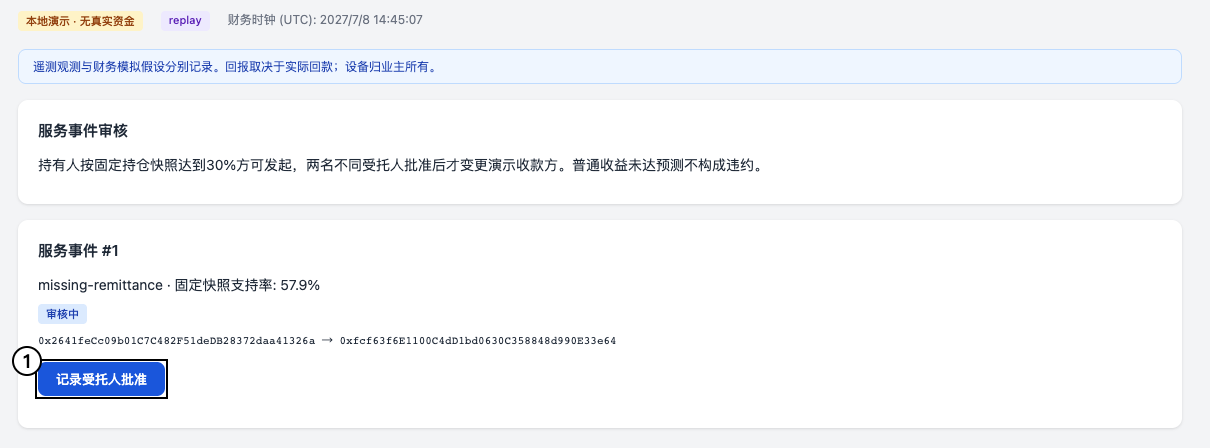
\includegraphics[width=\linewidth,height=.37\textheight,keepaspectratio]{assets/46-trustee-b-context.png}\par 编号标出操作位置。插图来自隔离演练，金额和状态以当前产品为准。\end{center}
\begin{center}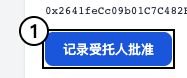
\includegraphics[width=.7\linewidth,height=1.55cm,keepaspectratio]{assets/46-trustee-b-detail.png}\end{center}
\end{landscape}
\clearpage\begin{landscape}
\section{到期关闭与凭证返还}
\subsection{H1 到期关闭产品}
本步由中介机构操作。进入“产品运营”的到期区后，确认60期费用与月度分配处理完成，应收款已收齐，负债结清，最终估值已批准，再点击编号1。

操作成功后，产品进入已关闭状态，剩余可用现金形成最终分配。下一步，投资者领取剩余分配。

关闭按钮不可用时应检查缺失条件，不能通过删除应收款或改写账本来强行关闭。

\begin{center}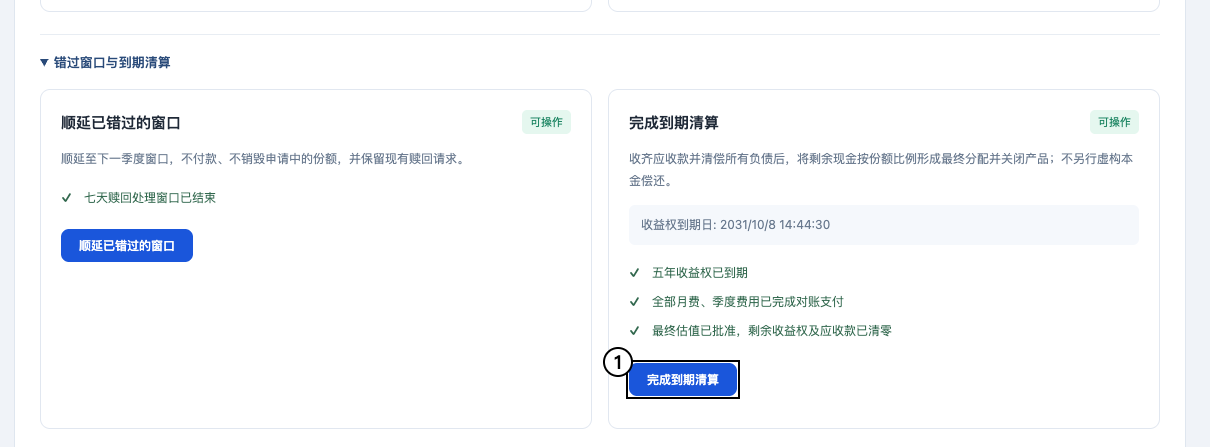
\includegraphics[width=\linewidth,height=.37\textheight,keepaspectratio]{assets/47-close-context.png}\par 编号标出操作位置。插图来自隔离演练，金额和状态以当前产品为准。\end{center}
\begin{center}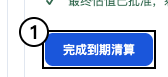
\includegraphics[width=.7\linewidth,height=1.55cm,keepaspectratio]{assets/47-close-detail.png}\end{center}
\end{landscape}
\clearpage\begin{landscape}
\subsection{H2 领取最终与尚未领取的分配}
本步由投资者A和B操作。进入“我的持仓”的分配记录后，逐笔核对尚未领取的金额，点击编号1并在钱包确认。

操作成功后，全部可领取USDC转入对应投资者钱包。下一步，业主取回站点凭证。

先前已经领取的月度分配不会再次支付。关闭后仍可能保留DRS数量作为份额历史记录，但不会因此延长已到期的收益权。最终分配也不是保证返还本金。

\begin{center}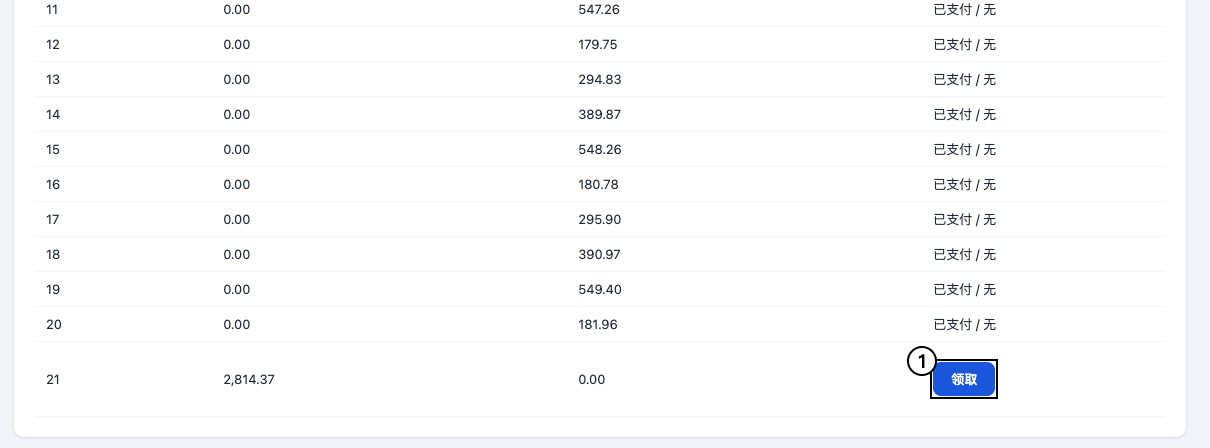
\includegraphics[width=\linewidth,height=.37\textheight,keepaspectratio]{assets/48-final-claim-context.png}\par 编号标出操作位置。插图来自隔离演练，金额和状态以当前产品为准。\end{center}
\begin{center}
\includegraphics[width=.7\linewidth,height=1.55cm,keepaspectratio]{assets/48-final-claim-detail.png}\end{center}
\end{landscape}
\clearpage\begin{landscape}
\subsection{H3 取回电站身份凭证}
本步由业主操作。进入“报价与协议”的到期待办后，确认对应产品已关闭，点击编号1签署取回交易。

操作成功后，站点NFT从资产池返回业主，收益权托管结束。下一步，本次业务闭环完成。

设备所有权此前一直属于业主。取回的是链上身份凭证，不是把真实设备重新卖给业主。

\begin{center}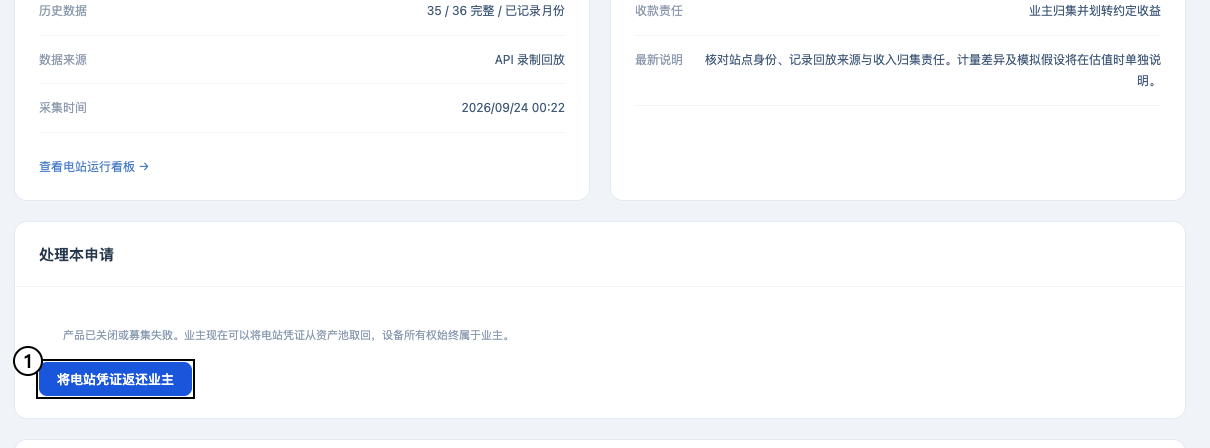
\includegraphics[width=\linewidth,height=.37\textheight,keepaspectratio]{assets/49-release-context.png}\par 编号标出操作位置。插图来自隔离演练，金额和状态以当前产品为准。\end{center}
\begin{center}
\includegraphics[width=.7\linewidth,height=1.55cm,keepaspectratio]{assets/49-release-detail.png}\end{center}
\end{landscape}
\clearpage\section{现金流计算与估值}
预测按最多36个月可用历史数据形成同月季节性基线，再按退化、可用率、上网行为和电价日程逐期调整。没有12个完整月时，报告明确标记为暂定估算，需要审核人说明原因。发电和上网不平衡的样本需要核查，不能简单把上网比例截为100\%后当作正常自用量。

\[S_t=\max(G_t-E_t,0)\,q_t,\qquad B_t=S_t\,p^{grid}_t\,d_t.\]
G表示预测发电量，E表示经核验的合资格售电量，q表示自用交付系数。S是可交付自用电量，B是业主按折扣比例d支付的电费。直接从电网购买这部分电量的比较费用为S乘电网价，优惠额为该比较费用减业主付款。这里只比较交付的光伏电量，不声称业主全部电网账单都会降低相同比例。

\[C_t=(B_t+E_t p^{export}_t-K_t)\,f_t\,a_t,\qquad V_0=\sum_{t=1}^{60}\frac{\widehat C_t}{(1+r)^{\tau_t/12}}.\]
K表示约定由收益权承担的站点成本，f为本币换USDC的演示汇率，a为签署协议的归集比例。新协议默认归集100\%，业主通过优惠电价保留利益。现金流按预计实际收款日期贴现，τ包含回款延迟。默认10\%名义年折现率是定价假设，不是承诺收益，报告同时比较6\%和14\%。

\clearpage\begin{landscape}
\subsection{前三期业主现金流时间轴}
\begin{center}\begin{tikzpicture}[>=Latex]\draw[->](0,0)--(22,0);
\fill(3,0)circle(2pt);\node[above]at(3,.2){第1期};
\fill(10,0)circle(2pt);\node[above]at(10,.2){第2期};
\fill(17,0)circle(2pt);\node[above]at(17,.2){第3期};
\end{tikzpicture}\end{center}\begin{center}\begin{tabular}{L{10cm}rrr}\toprule 计算项目 & 第1期 & 第2期 & 第3期\\\midrule
发电量 kWh & 3,861.20 & 4,307.49 & 3,732.04\\
售电量 kWh & 279.01 & 308.98 & 67.61\\
交付自用量 kWh & 3,223.97 & 3,598.66 & 3,297.99\\
直接电网比较费用 CNY & 1,934.38 & 2,159.19 & 1,978.80\\
业主优惠电费 CNY & 1,547.51 & 1,727.36 & 1,583.04\\
业主优惠额 CNY & 386.88 & 431.84 & 395.76\\
售电收入 CNY & 97.65 & 108.14 & 23.66\\
站点成本 CNY & 8.75 & 8.76 & 8.78\\
归集净应收 USDC & 229.10 & 255.74 & 223.71\\
折现现值 USDC & 225.48 & 249.68 & 216.64\\
\bottomrule\end{tabular}\end{center}
表中数值来自隔离产品的同一份估值报告，属于模型示例。完整报告覆盖60期，每期先分别计算业主电费、售电收入和成本，再按收款时间贴现求和。

\end{landscape}
\clearpage\begin{landscape}
\subsection{投资者前三个月现金流时间轴}
\begin{center}\begin{tikzpicture}[>=Latex]\draw[->](0,0)--(22,0);
\fill(1.0,0)circle(2pt);\node[above]at(1.0,.2){第0期投入};
\fill(7.5,0)circle(2pt);\node[above]at(7.5,.2){第1月};
\fill(14.0,0)circle(2pt);\node[above]at(14.0,.2){第2月};
\fill(20.5,0)circle(2pt);\node[above]at(20.5,.2){第3月};
\end{tikzpicture}\end{center}\begin{center}\begin{tabular}{L{11cm}rrr}\toprule 计算项目 & 第1月 & 第2月 & 第3月\\\midrule
预计收到现金 USDC & 0.00 & 229.10 & 255.74\\
计提年费部分 USDC & 6.04 & 6.09 & 6.06\\
必需月度池成本 USDC & 1.00 & 1.00 & 1.00\\
全池分配 USDC & 0.00 & 166.51 & 186.51\\
分配后池现金 USDC & 1,469.93 & 1,525.43 & 1,587.60\\
每投入1,000 USDC预计回款 & 0.00 & 11.27 & 12.63\\\bottomrule\end{tabular}\end{center}
初始认购款的10\%自动留在资金池，其余用于购买收益权。每个月在回款、费用与估值条件满足后宣告分配，并不表示每个月保证产生正分配。投资者还需要亲自领取。月度分配不改变六个月转让锁定和季度赎回窗口。

投资者净值由现金、可收回应收款和剩余收益权价值构成，再扣除负债及相应未来费用。已宣告分配单列，不能再作为可交易净值重复计算。年化净收益用初始投入、预计各次分配和到期剩余现金计算IRR。应同时看已领取现金、剩余NAV和总回报。

\end{landscape}
\clearpage\section{链上记录核对}
月度账单应分别核对BillPublished、HouseholdPaid、ExportFunded和ReceiptConfirmed。业主付款的发送者必须是本期业主，目标必须是该产品账单合约，金额必须等于账单应付值。确认入池交易由中介签署，并核对转给资产池的净额和一次性站点费用。已付款但未确认的资金仍在账单合约中，不能与资产池现金重复计算。

NFT铸造应核对站点Token ID和业主地址。授权应核对被授权Vault，入池应核对托管地址、协议摘要和购买价。估值审批应核对报告摘要、审批人和有效期。认购与结算应分别核对USDC转移、托管累计金额、发行DRS、业主收款和池内留存。

\begin{center}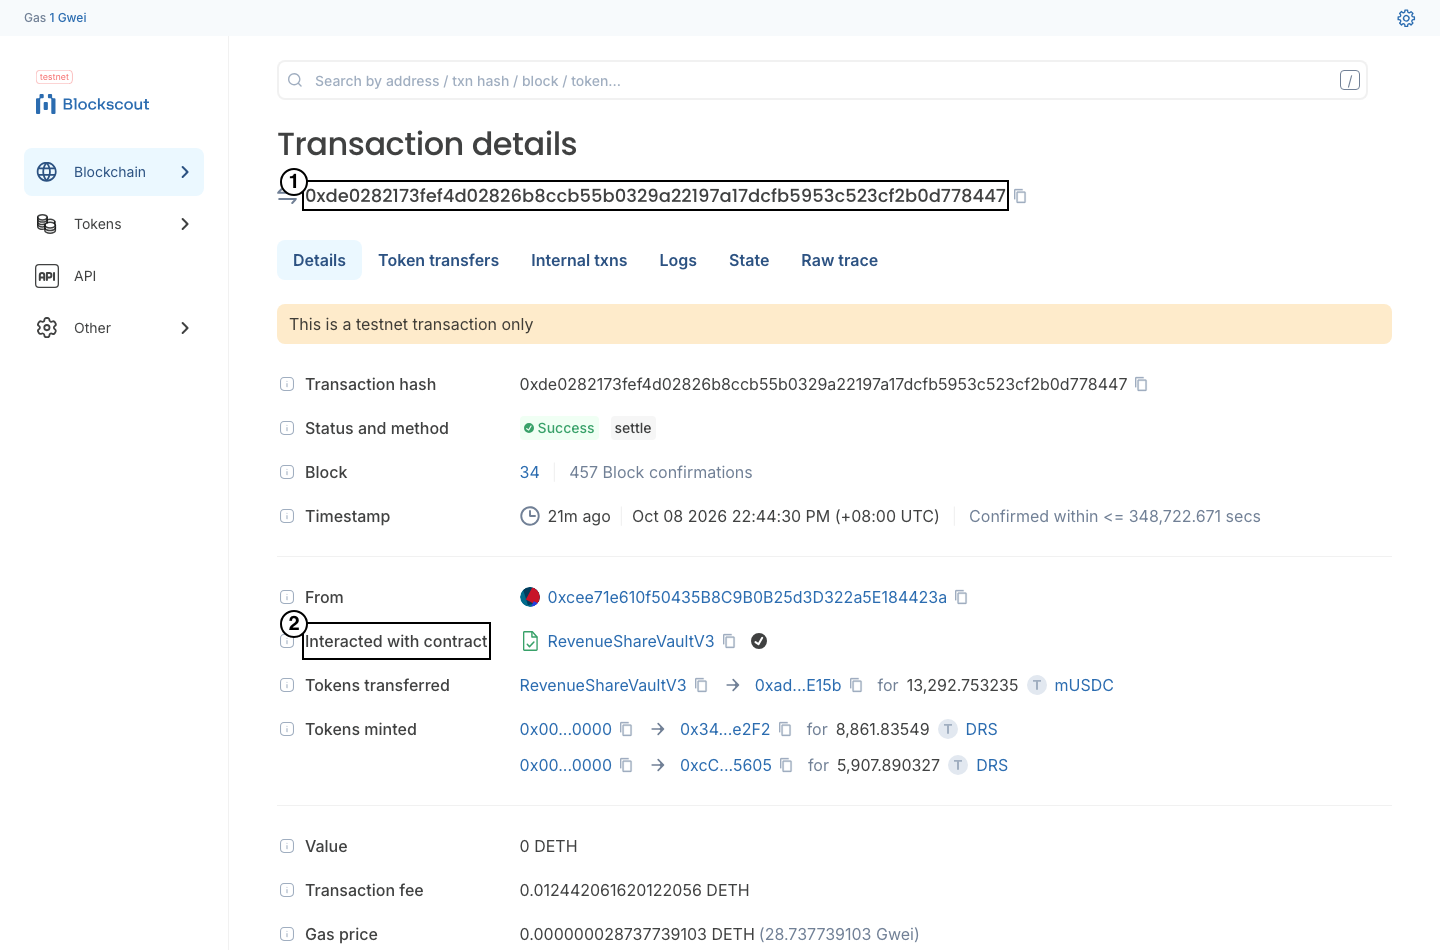
\includegraphics[width=\linewidth,height=.4\textheight,keepaspectratio]{assets/50-blockscout-transaction.png}\par 区块链浏览器交易详情示例。核对执行状态、发送者、目标合约和区块。\end{center}
\clearpage
分配宣告与领取是不同交易。前者形成持有人的领取权，后者把USDC转给指定投资者。转让应在同一回执核对DRS与USDC两条转移。赎回应核对实际成交份额、付款、销毁和剩余托管量。服务事件应核对快照、支持权重及两名独立审批地址。

\begin{center}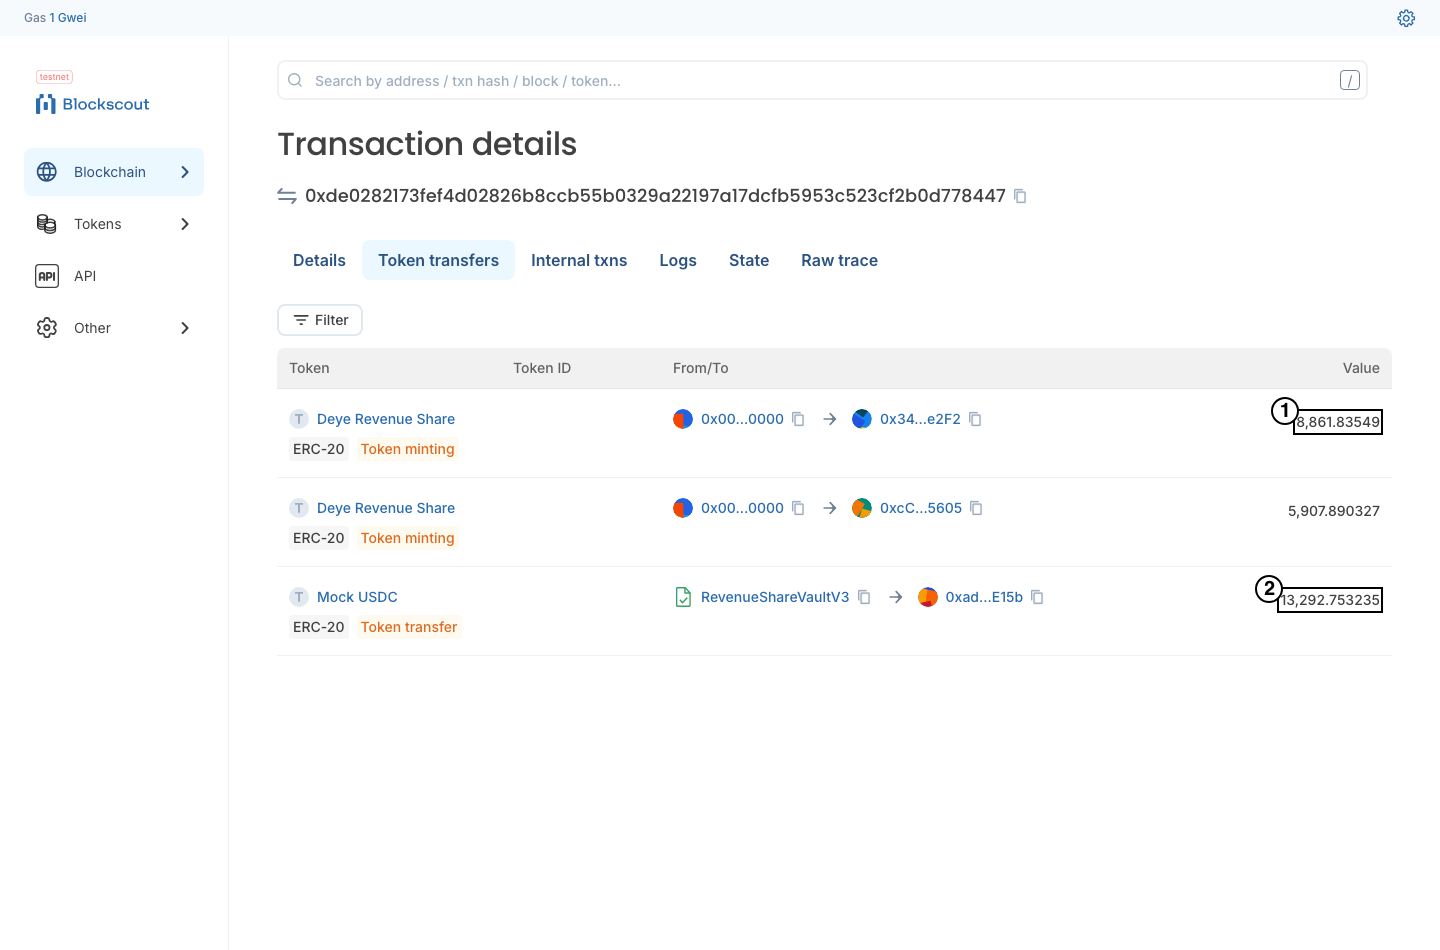
\includegraphics[width=\linewidth,height=.42\textheight,keepaspectratio]{assets/51-blockscout-events.png}\par 事件与代币记录示例。摘要只证明与链下资料的对应关系，不表示原始资料全部保存在链上。\end{center}
\clearpage\section{故障处理与测试边界}
\subsection{钱包或角色不匹配}
核对完整地址、链编号和当前角色。先在钱包切换账户，再重新选择角色并签名。不要通过反复点击角色按钮尝试获取权限。

\subsection{募集资金不足}
10\%是合约自动留存的初始现金。最低募集额通常需要覆盖购买价除以90\%的结果。按页面差额追加认购，再由中介重新审核，不能手动改账本绕过。

\subsection{估值或计费条件不足}
点击定位操作进入缺失条件的具体入口。报告过期或输入变化时由中介重新编制，再由受托批准。达到日期并不会自动满足净值审批。

\subsection{分配与余额未更新}
先确认是否已宣告本期分配，再检查本人可领取金额和历史已领取金额。USDC钱包余额、托管订单和投资净值分开显示。链上已确认但索引尚未完成时，保留哈希并稍后刷新。

\subsection{拒签、等待与恢复}
钱包拒签后可修改原操作并重试。已有交易哈希时先查询回执，不要再次支付。页面刷新和后台重启后应恢复原操作。测试链完全重建后，演示负责人需通知用户清理该测试网络的旧交易缓存。

\subsection{远程入口不可用}
GitHub静态首页仍可阅读，但业务、RPC和Blockscout依赖Mac、Docker及隧道运行。负责人使用remote:status检查，使用remote:start更新失效入口，再使用remote:publish更新公开配置。

\end{document}
